\chapter{RESULTADOS E DISCUSS\~AO}
\label{cap:capitulo4}

\section{Desempenho dos modelos}
%Apresentar e comparar os resultados dos diferentes modelos utilizados.

Os resultados obtidos pelos modelos apresentaram variações significativas em termos de precisão, tanto nas previsões pontuais quanto nos intervalos de confiança, refletindo diferentes graus de precisão para cada cenário analisado. A análise dos resíduos revelou-se particularmente interessante, pois evidenciou comportamentos distintos em função da sazonalidade, com variações marcantes observadas em diferentes períodos do ano.

\subsection{Rio Jequitinhonha}

Iniciando pela menor bacia hidrográfica estudada, os resultados revelaram-se bastante satisfatórios, especialmente no que se refere ao modelo de Regressão Linear, que se destacou com previsões precisas, tanto em termos pontuais quanto nos intervalos de confiança. Este modelo demonstrou uma capacidade robusta de capturar a dinâmica hidrológica do rio, refletindo precisão nas métricas e desempenho consistente, aliado a um tempo de execução significativamente reduzido. Em contrapartida, o modelo (simples) SeasonalNaive apresentou resultados abaixo das expectativas em todas as situações avaliadas - figura \ref{fig:jequiti_SN_WFV_ORIG}.

Com a MAPE extremamente elevada, de $150\%$, os resultados indicaram um viés significativo de superestimação, conforme evidenciado pela métrica PBIAS. Verificando a KGE, ficou negativa. Em outras palavras, isso significa que o modelo não apenas falha em capturar a variabilidade dos dados observados, mas também introduz erros que o tornam menos eficaz do que uma abordagem simplista, como utiilizar a média histórica. Embora a análise superficial da qualidade dos intervalos de confiança pudesse sugerir um desempenho satisfatório do modelo, uma inspeção mais detalhada revela uma incongruência: os valores inferiores do intervalo (lo-95) foram calculados abaixo de $0$, o que não faz sentido para o rio em questão, pois implicaria na ausência total de vazão, algo inviável para as condições medidas pela estação.

Considerando o desempenho insatisfatório do modelo SN, a análise foi encerrada neste ponto, sem proceder com a avaliação dos resíduos ou a análise da importância das variáveis. O modelo foi incluído apenas para fins comparativos. A análise mais aprofundada será dedicada aos modelos mais complexos, que apresentaram desempenho superior.

\begin{figure}[!h]
	\centering
	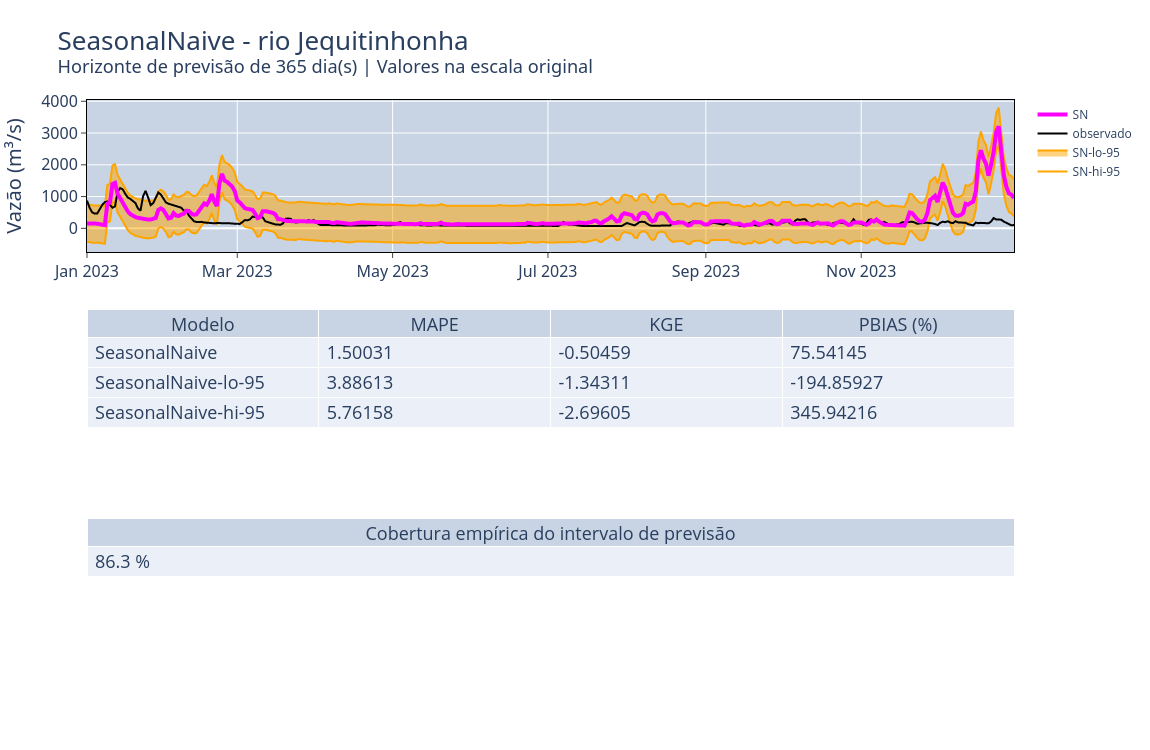
\includegraphics[scale=0.33]{Figuras/jequiti/wfv/SN/SN_WFV_ORIG.png}
	\caption{Resultado do SeasonalNaive no teste \textit{Walk-Forward Validation}\\(fonte: o autor)}
	\label{fig:jequiti_SN_WFV_ORIG}
\end{figure}
\clearpage

Os resultados obtidos utilizando o modelo LR mostraram-se bastante promissores - figura \ref{fig:jequiti_LR_WFV_LOG}. Nesta primeira avaliação, os dados foram log-transformados. Isso é verificável pelo título com o uso de ``destransformados''. Os dados foram log-transformados e retornados para a escala original para desenhar o gráfico e ficarem acessíveis para quem lê. \underline{Essa dinâmica no título se manterá por todo trabalho}.

Partindo pela KGE calculada, o resultado mostrou-se excelente. Recordando: quanto mais próxima de $1$, melhor. Este valor sugere que o modelo foi eficaz na previsão do comportamento hidrológico do sistema em análise, oferecendo previsões que estão bem alinhadas com os dados observados. A MAPE de $14,5\%$ sugere que o modelo tem uma precisão média absoluta razoável e é bastante confiável. O modelo apresentou um viés sistemático de subestimar os resultados, conforme aponta a PBIAS de $-0,97\%$. Considerando todas as métricas, o resultado indica que o modelo teve um desempenho global muito bom. A KGE alta é particularmente indicativa de um bom ajuste global, com o modelo capturando bem tanto a dinâmica quanto a magnitude dos dados observados.

Considerando a qualidade dos intervalos de previsão, a cobertura observada de $98,08\%$ excedeu o intervalo teórico calculado de $95\%$, o que, à primeira vista, poderia ser interpretado como um desempenho satisfatório. No entanto, o limite superior do intervalo (hi-95) mostrou-se excessivamente elevado nos meses de janeiro e fevereiro, o que pode comprometer a interpretação dos resultados. Isso ocorre porque intervalos de previsão excessivamente amplos podem capturar praticamente qualquer valor observado, reduzindo a utilidade prática da previsão.

É importante destacar que os intervalos de previsão são calculados a partir dos erros do modelo durante a etapa de treinamento (\textit{bootstrap in-sample residuals}). Para uma análise mais aprofundada desse comportamento, é necessário examinar os dados anteriores a $2023$. A figura \ref{fig:jequiti_LR_final_2022_detalhe} revela que, nos últimos dias de $2022$, houve observações significativamente elevadas. É provável que os erros associados a esse período mais próximo tenham influenciado a amplitude dos intervalos de previsão subsequentes. Essa interpretação é suportada pela observação de que o comportamento ao final de $2023$ foi mais estável, possivelmente devido à ausência de eventos ruidosos imediatamente anteriores - meses de maio a agosto.

\begin{figure}[!h]
	\centering
	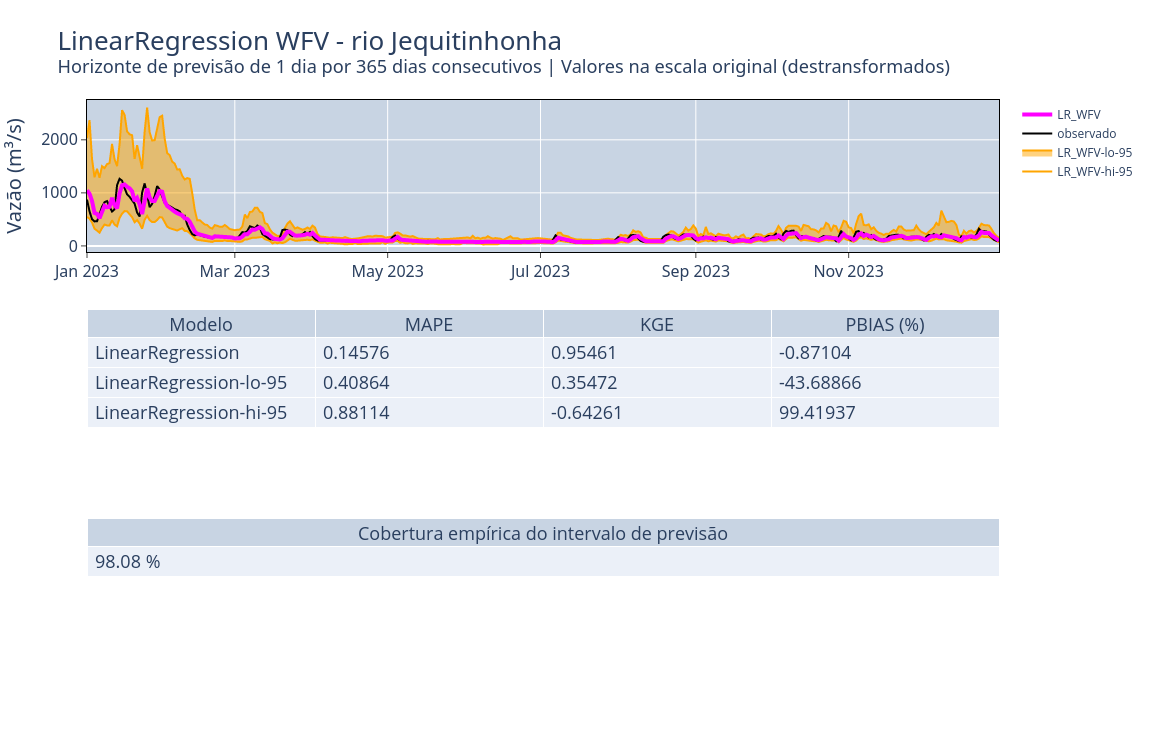
\includegraphics[scale=0.33]{Figuras/jequiti/wfv/LR/LR_WFV_LOG.png}
	\caption{\textit{Walk-Forward Validation} para o modelo Regressão Linear - LR\\(fonte: o autor)}
	\label{fig:jequiti_LR_WFV_LOG}
\end{figure}

\begin{figure}[!h]
	\centering
	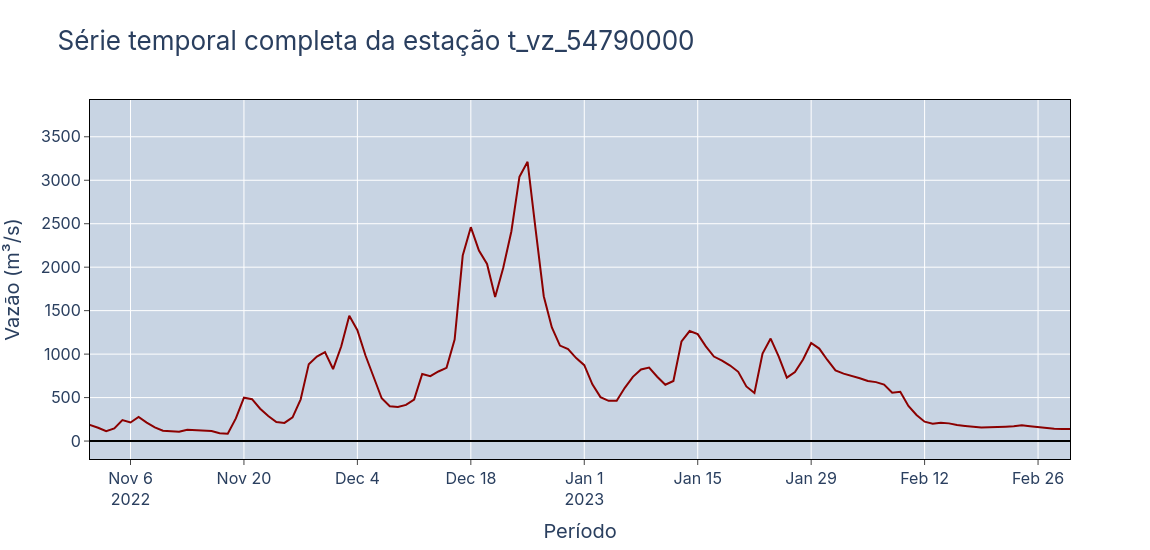
\includegraphics[scale=0.33]{Figuras/jequiti/LR_final_2022_detalhe.png}
	\caption{Detalhe do trecho final dos dados, em 2022, usados para treinamento.\\(fonte: o autor)}
	\label{fig:jequiti_LR_final_2022_detalhe}
\end{figure}

%A análise de \textit{delay} mostrou um resultado médio de $-0,87$. Se pegar a série prevista pelo modelo e comprimir linearmente em $-0,87$, ambas as sequências serão idênticas, ou seja, a série prevista será a série observada. Considerando que os dados estão numa frequência diária, isso pode ser interpretado como o modelo atrasando a previsão em $0,87$ dias, o que seria menos de 24 horas entre o evento ocorrer e ele ser percebido na previsão. Afirmar que o modelo está atrasado 20,88 horas, talvez, não convirja com a realidade, por isso que se considerar o desvio-padrão no resultado, confere mais coerência, pois indicaria que o atraso percebido no fenômeno é de cerca de um dia e meio, dois dias.

%\begin{figure}[!h]
%\centering
%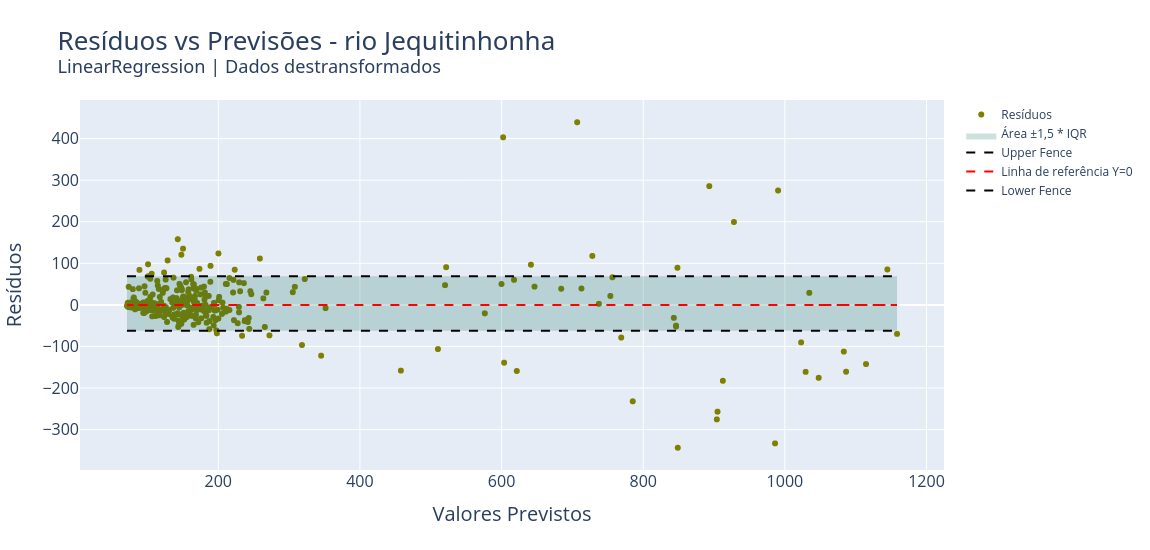
\includegraphics[scale=0.33]{Figuras/jequiti/wfv/LR/LR_WFV_LOG_RESID_x_PREV.png}
%\caption{Dispersão dos resíduos.\\(fonte: o autor)}
%\label{fig:jequiti_LR_WFV_LOG_RESID_x_PREV}
%\end{figure}
%
%Na figura \ref{fig:jequiti_LR_WFV_LOG_RESID_x_PREV} podemos observar a concentração dos resíduos em torno de zero. A linha vermelha tracejada é onde o valor previsto e observado são iguais, designando a previsão perfeita, com resíduo $0$. Este é o comportamento que se espera, idealmente, os resíduos estarem distribuídos aleatoriamente em torno de zero, sem padrões evidentes (nenhuma tendência clara de curvatura ou cone). Contudo, à medida que se caminha sobre a linha vermelha tracejada, aumentando o valor no eixo x, há um aumento na dispersão dos resíduos.

A área sombreada demarcada na figura \ref{fig:jequiti_LR_WFV_LOG_RESID_x_TEMPO} são os valores calculados para \textit{lower fence} e \textit{upper fence} - como se vê em um \textit{boxplot} - a partir do primeiro ($-12,83$) e terceiro ($19,98$) quartil, que aqui resultaram em $-62,06$ e $69,21$, respectivamente. Entre estes valores é onde se espera que os resíduos estejam distribuídos (houve uma prevalência de $87,4\%$ dos resíduos nesta área), o que fica de fora dessas faixas pode ser interpretado como um \textit{outlier}. Considerando que os dados de treinamento não foram tratados para valores \textit{outliers}, isso parece estar se refletindo neste resultado, mesmo com a transformação logarítmica. O modelo não captou corretamente os valores elevados nos dados observados, por isso resíduos tão grandes assim, ainda que tenha apresentado um comportamento geral bom, como visto nas métricas anteriormente. Outro fator a se considerar também é que por estar na escala log, qualquer pequena variação nesta escala, quando retornada para a escala original, pode gerar números elevados.

Nesta mesma figura \ref{fig:jequiti_LR_WFV_LOG_RESID_x_TEMPO} vê-se como os resíduos estão dispersos ao longo do tempo. Isso ajuda a compreender a estabilidade do modelo. No início do ano e final do ano, exatamente quando os eventos de chuva mais ocorrem, o comportamento geral de vazões torna-se incerto e o modelo tende a se espalhar mais. No início do ano, como discutido anteriormente, pode ser que devido às vazões elevadas do final do ano de $2022$, isso tenha causado ruídos em excesso na previsão do modelo. Quando houve vazões mais moderadas, os resíduos foram também mais moderados, como pode-se observar no final do ano de 2023, em que a influência imediata é o meio do ano, meses de inverno, e início de primavera. Quando da estação de baixa dos rios, os meses de outono e inverno, os resíduos estiveram bem alinhados em torno do $0$.

Para encerrar essa análise, a figura \ref{fig:jequiti_LR_WFV_LOG_RESID_x_CURVA_NORMAL} apresenta que os resíduos estão próximos da normalidade quanto à distribuição destes em torno de $0$, com uma assimetria de $0,48$. O valor positivo para assimetria sugere que houve casos em que o modelo subestimou os valores na previsão (existe uma cauda à direita do centro dos dados), o que combina com a métrica PBIAS. Mas cabe destacar que os resíduos não estão significativamente desviados em nenhuma direção, apresentam distribuição concentrada em torno de $0$ e este é um comportamento desejado. A análise da função de autocorrelação (ACF) está na figura \ref{fig:jequiti_LR_WFV_LOG_RESID_ACF} e aqui é analisado se existe independência ou dependência temporal entre os resíduos. A área sombreada representa a faixa ideal de permanência dos resíduos, onde se espera que a maioria dos resíduos esteja concentrada caso não haja autocorrelação significativa. Algumas \textit{lags} estão fora destes limites (picos), mais precisamente, \textit{lags} que estão mais próximas da \textit{lag} de referência. Este comportamento indica que o modelo pode ser refinado para melhor capturar dinâmicas temporais, possivelmente incorporando termos de tendência. Mas no aspecto geral, está bom o comportamento dos resíduos. Para melhorar os resíduos com valores tão elevados um tratamento de \textit{outliers} pode verter bons resultados.

\begin{figure}[!h]
	\centering
	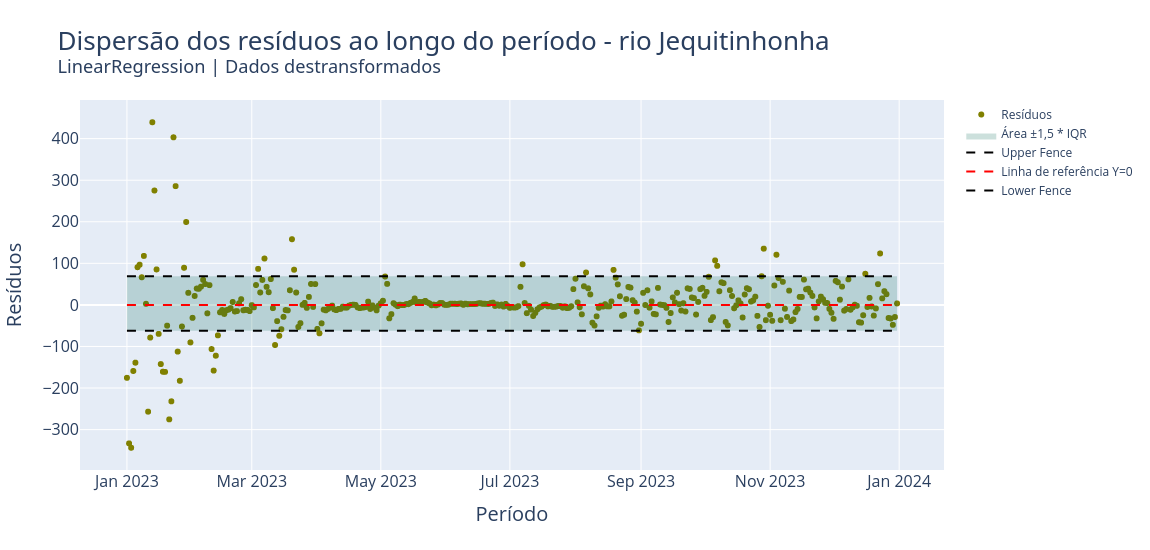
\includegraphics[scale=0.33]{Figuras/jequiti/wfv/LR/LR_WFV_LOG_RESID_x_TEMPO.png}
	\caption{Resíduos da previsão ao longo do tempo.\\(fonte: o autor)}
	\label{fig:jequiti_LR_WFV_LOG_RESID_x_TEMPO}
\end{figure}

\begin{figure}[!h]
	\centering
	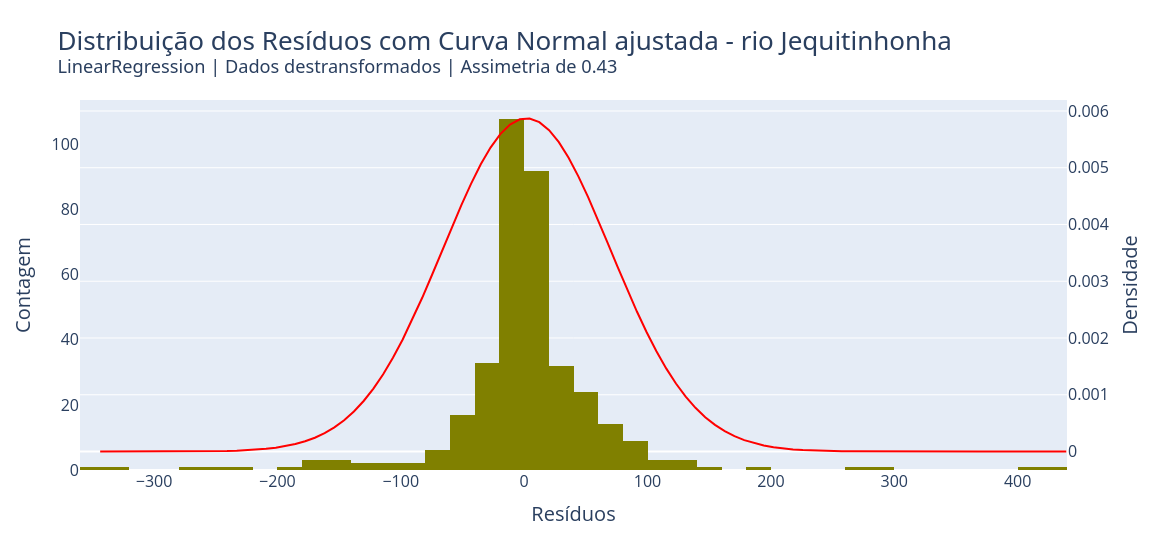
\includegraphics[scale=0.33]{Figuras/jequiti/wfv/LR/LR_WFV_LOG_RESID_x_CURVA_NORMAL.png}
	\caption{Histograma dos resíduos.\\(fonte: o autor)}
	\label{fig:jequiti_LR_WFV_LOG_RESID_x_CURVA_NORMAL}
\end{figure}

\begin{figure}[!h]
	\centering
	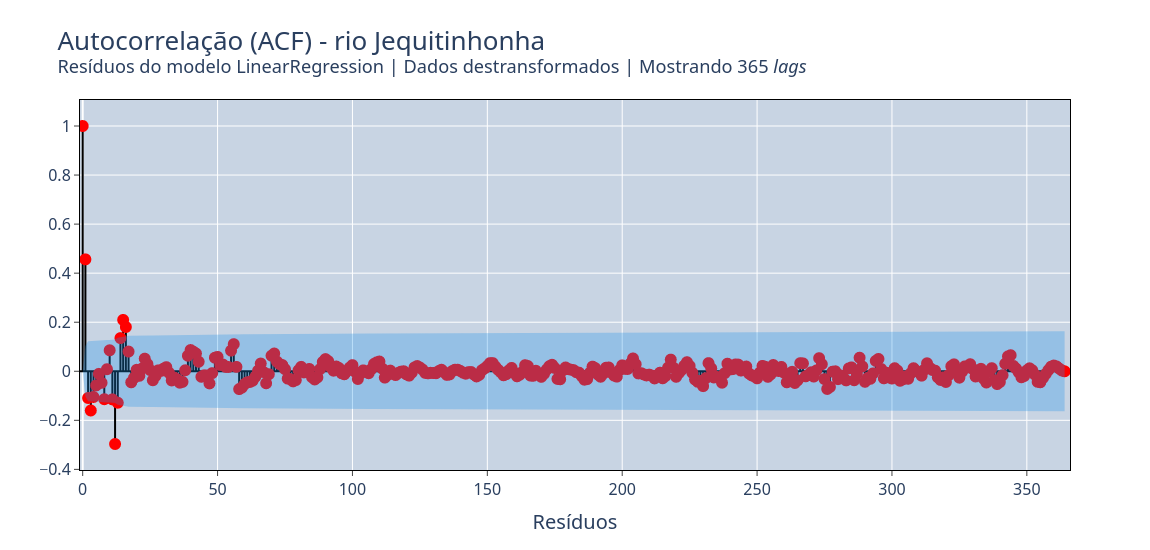
\includegraphics[scale=0.33]{Figuras/jequiti/wfv/LR/LR_WFV_LOG_RESID_ACF.png}
	\caption{Resíduos da previsão ao longo do tempo.\\(fonte: o autor)}
	\label{fig:jequiti_LR_WFV_LOG_RESID_ACF}
\end{figure}
\clearpage

Passando agora à análise dos modelos principais deste trabalho, cujos resultados serão comparados ao modelo de referência - o modelo \textit{LinearRegression} -, optou-se por realizar a análise de forma concomitante, uma vez que ambos os modelos apresentaram comportamentos similares, embora o modelo RF tenha demonstrado um desempenho superior ao CB. Neste ponto, os resultados dos modelos não-lineares passaram pela log-transformação.

Na métrica KGE, comparando-se os resultados com o comportamento visto na figura \ref{fig:jequiti_LR_WFV_LOG}, observa-se que ambos os modelos não conseguiram superar o modelo de referência, com destaque para o CB, que apresentou uma performance consideravelmente inferior - figuras \ref{fig:jequiti_CB_WFV_LOG} e \ref{fig:jequiti_RF_WFV_LOG}. No entanto, ao considerar a previsão percentual média, avaliada pela métrica MAPE, ambos os modelos baseados em árvores apresentaram melhorias em relação ao modelo de referência, evidenciando um desempenho superior em termos de erro percentual médio.

A KGE, relembrando, combina três aspectos fundamentais: variabilidade, viés e correlação entre os dados observados e previstos. Considerando esses fatores, com os dados log-transformados, o modelo LR capturou de forma mais eficaz os três aspectos mencionados. É provável que a linearização tenha sido um fator determinante para o bom desempenho do modelo LR olhando por esta métrica, uma vez que, ao analisar a MAPE, os modelos não-lineares (CB com $0,13$ e RF com  $0,12$) apresentaram desempenhos melhores. Um desempenho médio percentual melhor pode dever-se à resiliência dos modelos não-lineares à sua robustez diante de valores discrepantes, aos quais o modelo linear é mais sensível.

Observa-se que tanto o CB quanto o RF apresentaram intervalos de previsão menos amplos no início do ano, em comparação com o modelo LR, mesmo impactados pelas vazões elevadas no final de $2022$ (figura \ref{fig:jequiti_LR_final_2022_detalhe}). Em termos de previsão pontual, ambos os modelos não-lineares demonstraram-se robustos, no entanto, ao analisar a cobertura empírica dos intervalos de previsão, o modelo RF mostrou-se consideravelmente defasado em relação aos modelos LR e CB. Isso pode ser explicado pela possível ``otimização'' excessiva do modelo ao calcular os intervalos, ao presumir uma repetição dos eventos e erros passados, resultando em intervalos estreitos. Esse fenômeno é explicado por \citet{RobHyndman_prediction_intervals}. Apesar disso, a cobertura empírica de $80\%$ do modelo RF ainda pode ser considerada satisfatória, e a cobertura de $86\%$ obtida pelo CB demonstra um bom desempenho.

%Pode-se inferir que os modelos CB e RF conseguiram equilibrar a previsão pontual, indicada pela MAPE de $0,12$, com os intervalos de previsão. Um ajuste de hiperparâmetros poderia potencialmente melhorar esse desempenho. Em relação ao PBIAS, ambos os modelos apresentaram um desvio sistemático, subestimando os valores previstos.

\begin{figure}[!h]
	\centering
	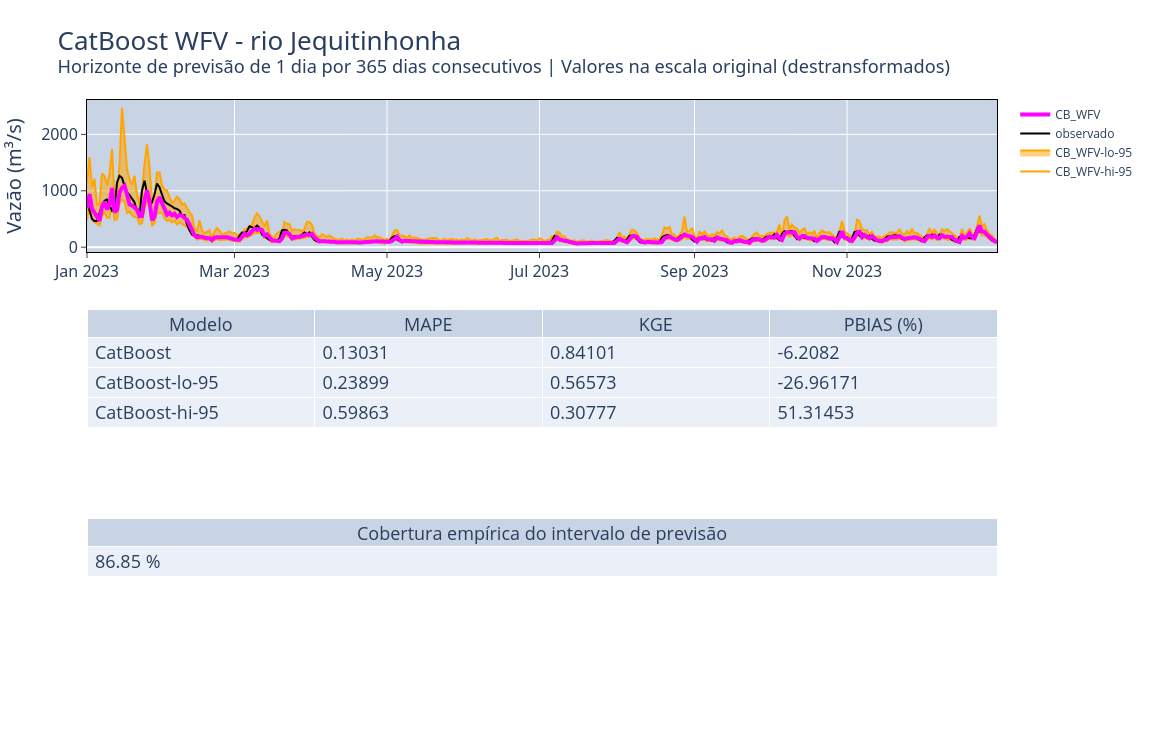
\includegraphics[scale=0.33]{Figuras/jequiti/wfv/CB/CB_WFV_LOG.png}
	\caption{\textit{Walk-Forward Validation} para o modelo CatBoost - CB.\\(fonte: o autor)}
	\label{fig:jequiti_CB_WFV_LOG}
\end{figure}

\begin{figure}[!h]
	\centering
	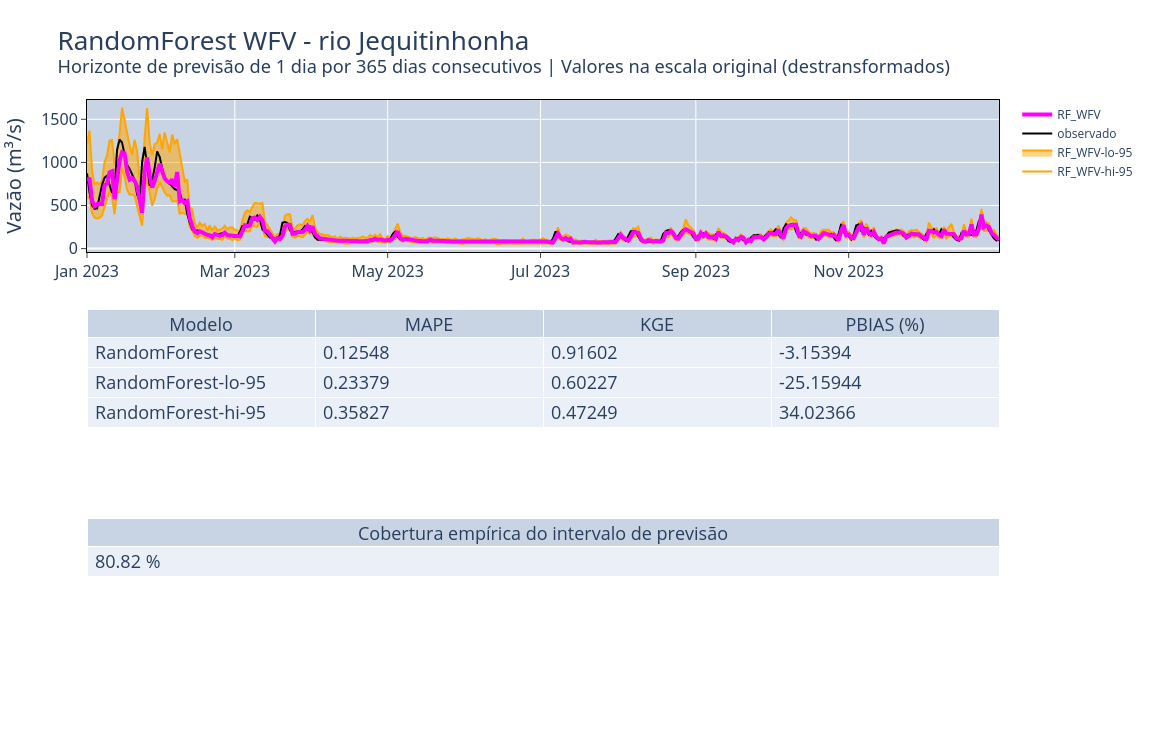
\includegraphics[scale=0.33]{Figuras/jequiti/wfv/RF/RF_WFV_LOG.png}
	\caption{\textit{Walk-Forward Validation} para o modelo RandomForest - RF.\\(fonte: o autor)}
	\label{fig:jequiti_RF_WFV_LOG}
\end{figure}
\clearpage

Os resíduos em modelos não-lineares podem ser mais difíceis de interpretar porque esses modelos capturam interações e padrões complexos. Porém, mesmo assim, detectar padrões sistemáticos nos resíduos ajuda a elucidar se os modelos conseguiram capturar todas as nuances dos dados.

%Em ambos os casos, não houve prevalência de comportamento anormal para os resíduos. Estiveram aleatoriamente distribuídos em torno de $0$, com uma menção importante para a maior dispersão de possíveis valores \textit{outliers} para o modelo CB à medida que as medições aumentaram.(figura \ref{fig:jequiti_CB_WFV_LOG_RESID_x_PREV}).
%
%\begin{figure}[!h]
%\centering
%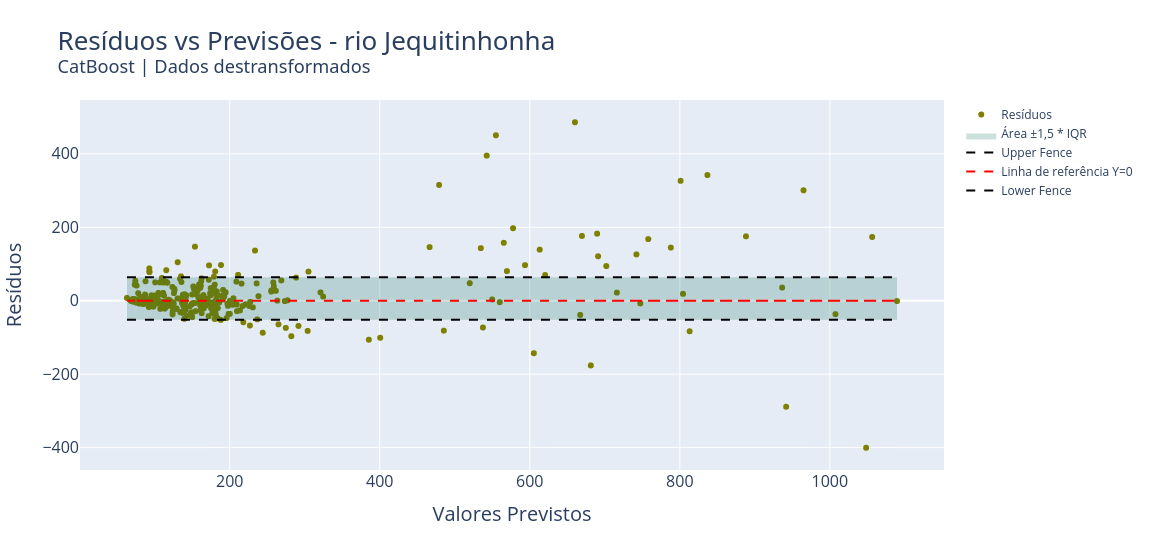
\includegraphics[scale=0.33]{Figuras/jequiti/wfv/CB/CB_WFV_LOG_RESID_x_PREV.png}
%\caption{Dispersão dos resíduos.\\(fonte: o autor)}
%\label{fig:jequiti_CB_WFV_LOG_RESID_x_PREV}
%\end{figure}
%
%\begin{figure}[!h]
%\centering
%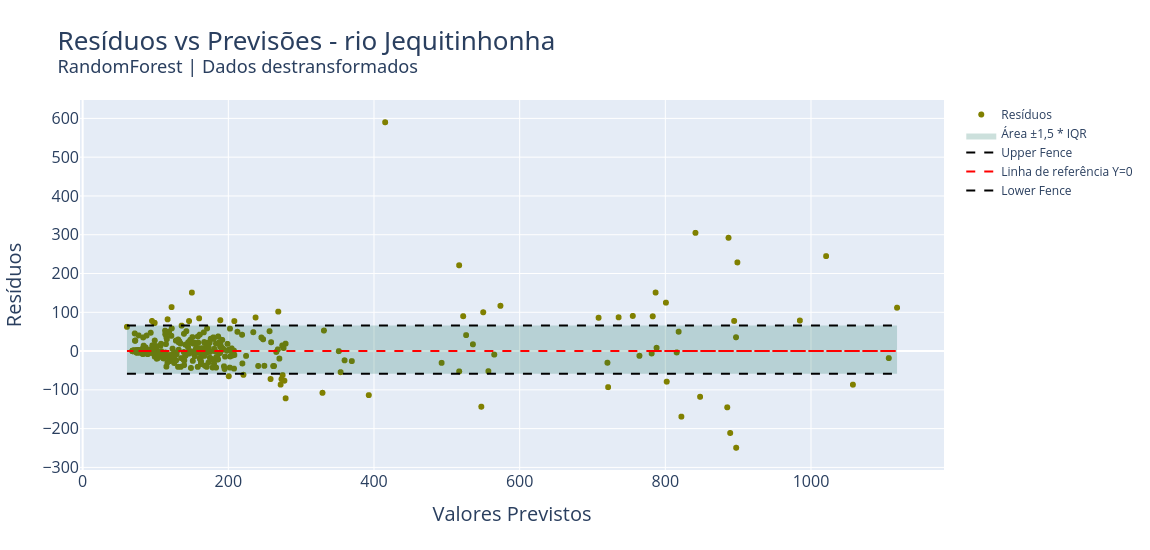
\includegraphics[scale=0.33]{Figuras/jequiti/wfv/RF/RF_WFV_LOG_RESID_x_PREV.png}
%\caption{Dispersão dos resíduos.\\(fonte: o autor)}
%\label{fig:jequiti_RF_WFV_LOG_RESID_x_PREV}
%\end{figure}
%\clearpage

A dispersão ao longo do tempo foi praticamente a mesma para ambos os modelos, com resíduos de valor elevado mais presentes no início da série - figuras \ref{fig:jequiti_CB_WFV_LOG_RESID_x_TEMPO} e \ref{fig:jequiti_RF_WFV_LOG_RESID_x_TEMPO}. Aqui vale a interpretação usada para o modelo de referência, de que os valores elevados aferidos em final de $2022$ possam ter interferido. Houve uma prevalência de $84,11\%$ e $86,03\%$, respectivamente CB e RF, dos resíduos na área sombreada, correspondente a $\pm 1,5 \times IQR$, que é onde se espera que todos os resíduos estejam - \textit{upper fence} e \textit{lower fence} do boxplot. Uma leve melhor prevalência para o modelo RF, que pode ser vista também em menos dispersão de resíduos para fora dos limites da área sombreada no início do ano.

\begin{figure}[!h]
	\centering
	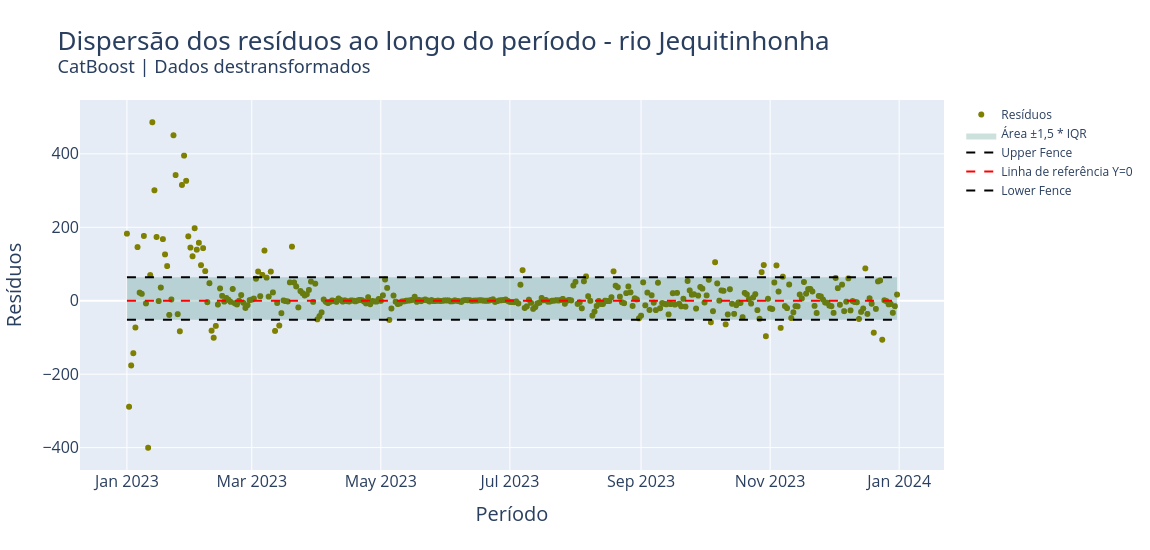
\includegraphics[scale=0.33]{Figuras/jequiti/wfv/CB/CB_WFV_LOG_RESID_x_TEMPO.png}
	\caption{Dispersão dos resíduos ao longo do ano.\\(fonte: o autor)}
	\label{fig:jequiti_CB_WFV_LOG_RESID_x_TEMPO}
\end{figure}

\begin{figure}[!h]
	\centering
	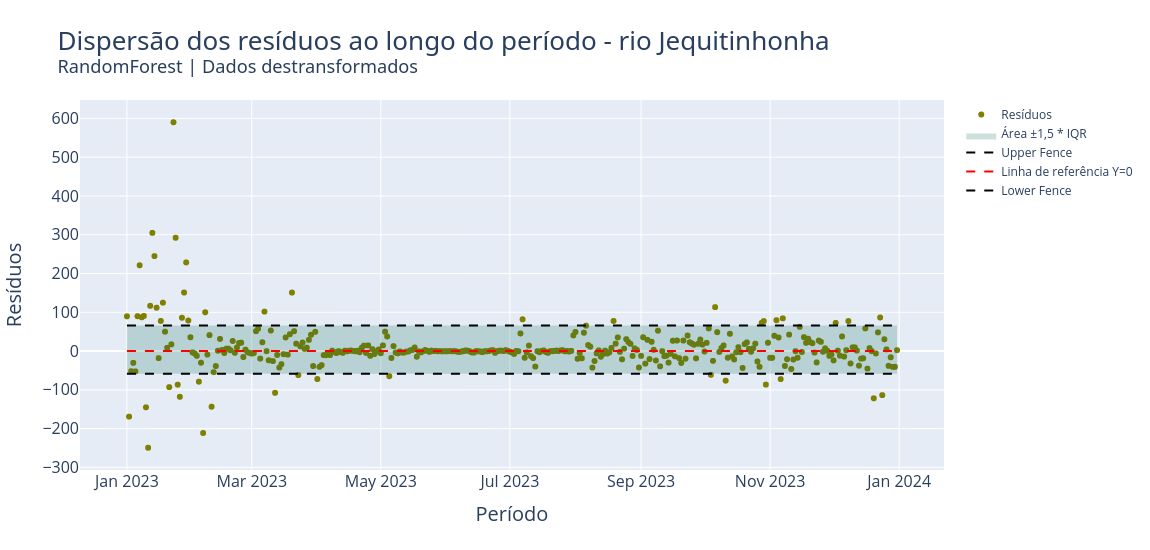
\includegraphics[scale=0.33]{Figuras/jequiti/wfv/RF/RF_WFV_LOG_RESID_x_TEMPO.png}
	\caption{Dispersão dos resíduos ao longo do ano.\\(fonte: o autor)}
	\label{fig:jequiti_RF_WFV_LOG_RESID_x_TEMPO}
\end{figure}
\clearpage

Em termos de assimetria da distribuição dos resíduos, ambos modelos apresentaram valores elevados, com assimetria positiva indicando cauda à direita. Com valores de $2,02$ para o modelo CB e $3,05$ para o RF, isso mostra tendência de subestimar as previsões, como visto anteriormente pelo PBIAS de ambos os modelos.

\begin{figure}[!h]
	\centering
	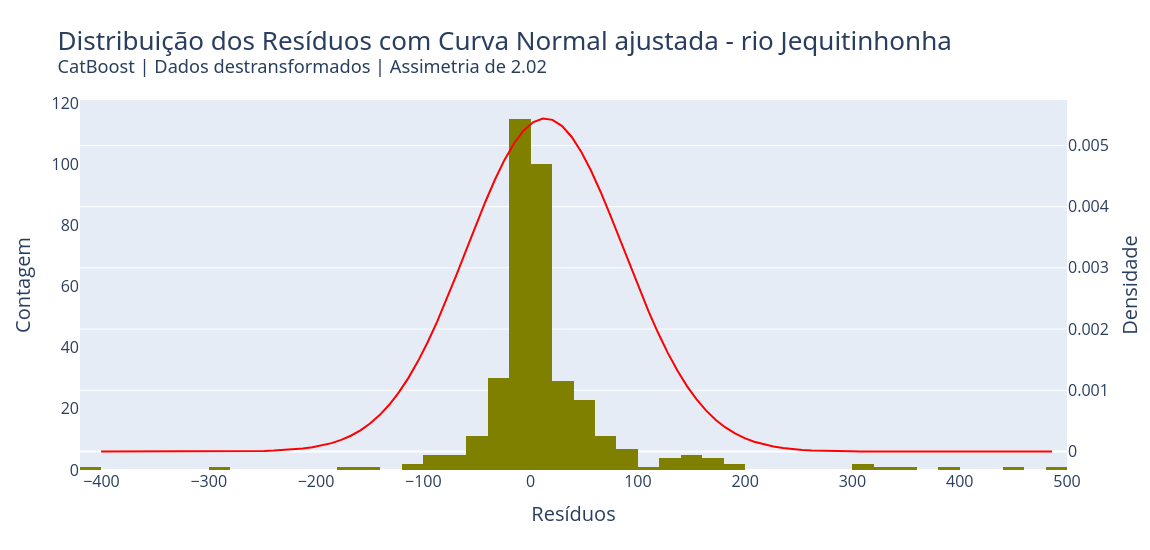
\includegraphics[scale=0.33]{Figuras/jequiti/wfv/CB/CB_WFV_LOG_RESID_x_CURVA_NORMAL.png}
	\caption{Histograma e curva-normal dos resíduos.\\(fonte: o autor)}
	\label{fig:jequiti_CB_WFV_LOG_RESID_x_CURVA_NORMAL}
\end{figure}

\begin{figure}[!h]
	\centering
	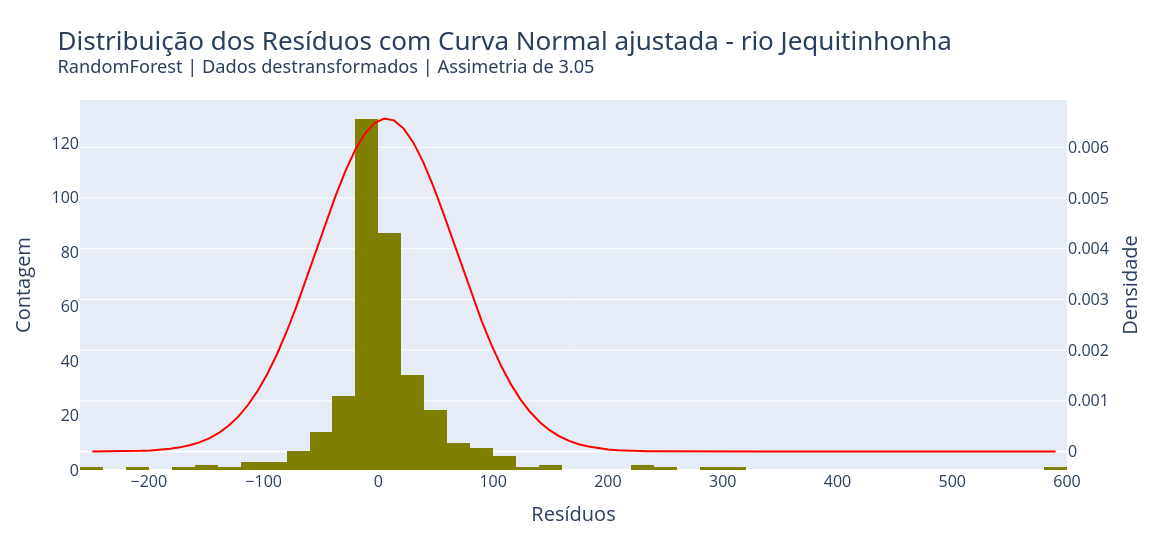
\includegraphics[scale=0.33]{Figuras/jequiti/wfv/RF/RF_WFV_LOG_RESID_x_CURVA_NORMAL.png}
	\caption{Histograma e curva-normal dos resíduos.\\(fonte: o autor)}
	\label{fig:jequiti_RF_WFV_LOG_RESID_x_CURVA_NORMAL}
\end{figure}
\clearpage

Observando os gráficos de autocorrelação dos modelos, houve um comportamento parecido nas \textit{lags} iniciais. Nas primeiras \textit{lags}, os gráficos mostram pontos de autocorrelação que ultrapassam a faixa de confiança - sombreada em azul -, indicando que os resíduos possuem dependência temporal significativa nos primeiros períodos. Esse padrão sugere que os modelos não conseguiram capturar totalmente a estrutura temporal dos dados, resultando em resíduos correlacionados em curtos períodos de tempo. Uma possível explicação pode ser a presença de componentes sazonais ou padrões de curto prazo que não foram completamente modelados e capturados pelos modelos.

A partir de aproximadamente a \textit{lag} $20$, a autocorrelação dos resíduos cai para valores próximos de $0$ e permanece dentro da faixa de confiança para as \textit{lags} seguintes até a \textit{lag} $365$. Este é um comportamento esperado para um bom modelo, onde os resíduos devem ser independentes e distribuídos aleatoriamente ao longo do tempo. A presença de resíduos com baixa autocorrelação em \textit{lags} mais próximas - ao início - indica que, em períodos mais longos, os modelos não apresentam problemas de dependência temporal.

\begin{figure}[!h]
	\centering
	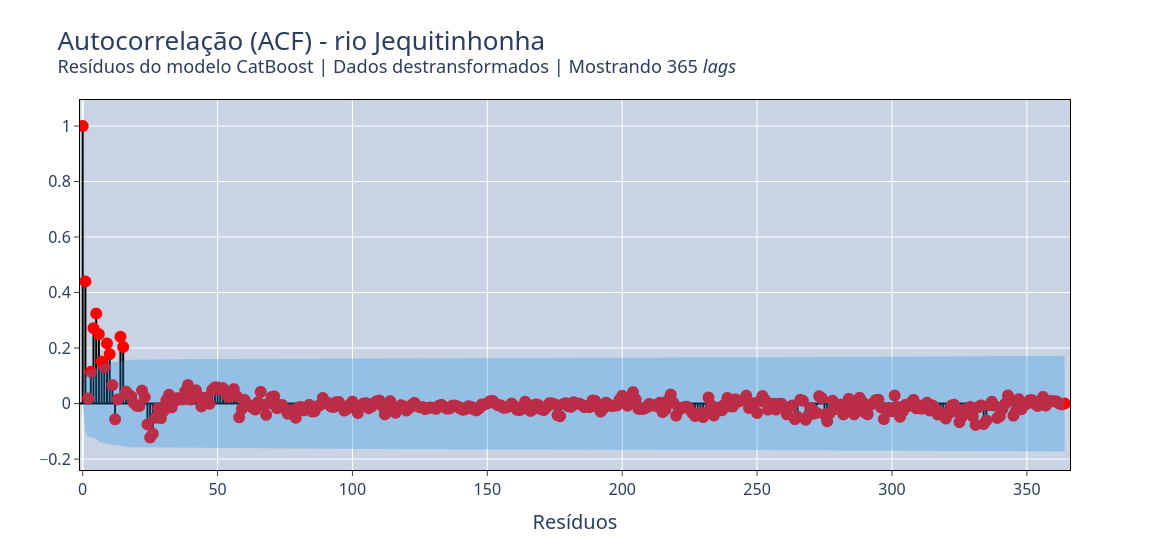
\includegraphics[scale=0.33]{Figuras/jequiti/wfv/CB/CB_WFV_LOG_RESID_ACF.png}
	\caption{Gráfico ACF dos resíduos.\\(fonte: o autor)}
	\label{fig:jequiti_CB_WFV_LOG_RESID_ACF}
\end{figure}

\begin{figure}[!h]
	\centering
	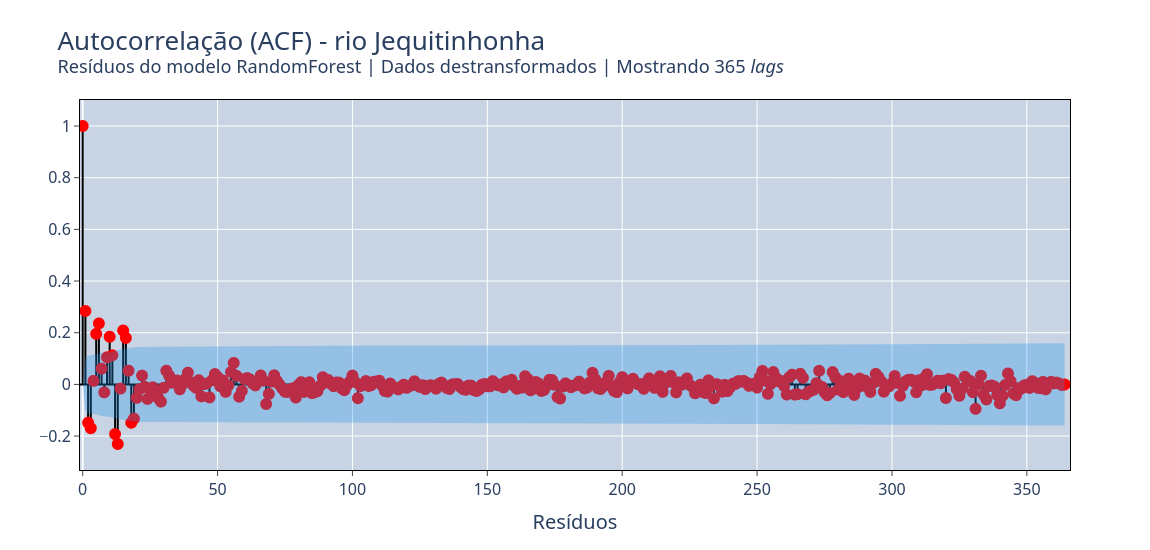
\includegraphics[scale=0.33]{Figuras/jequiti/wfv/RF/RF_WFV_LOG_RESID_ACF.png}
	\caption{Gráfico ACF dos resíduos.\\(fonte: o autor)}
	\label{fig:jequiti_RF_WFV_LOG_RESID_ACF}
\end{figure}
\clearpage

Agora os resultados sem emprego de log-transformação, com os dados originais. Salientando que para o modelo LR não é correto aplicar os dados originais na escala em que se encontram, foi preciso realizar normalização antes empregando algoritmo MinMax. Este algoritmo coloca todos os dados em valores entre $0$ e $1$, sendo o valor mínimo correspondente de cada série temporal passado para $0$ e o valor máximo, consequentemente, é passado para $1$. Com os demais valores é feito, basicamente, uma regra de três para achar o valor correspondente na escala entre $0$ e $1$.

Dito isso, o resultado para os dados originais ficou levemente inferior em relação ao modelo com os dados log-transformados. Em todas as métricas que se avaliar o resultado ficou piorado. Um comportamento destacado foi as faixas nos valores dos intervalos de previsão. Diferentemente do comportamento anterior - figura \ref{fig:jequiti_LR_WFV_LOG} -, em que houve uma prevalência de faixas elevadas no início do ano, neste resultado o início do ano esteve, digamos, bem comportado. Ao decorrer do ano que os intervalos incrementaram, a partir do mês de fevereiro, e foram aumentando até o fim do ano. Isso pode ser um indicativo de que o modelo teve problemas na estabilidade de longo prazo, acumulando as incertezas no período.

Ainda que tenha apresentado uma KGE inferior, bem como nas demais métricas, quando se observa o comportamento dos resíduos, houve uma prevalência de $91,78\%$ dos resíduos na área sombreada no gráfico \ref{fig:jequiti_LR_WFV_ORIG_RESID_x_TEMPO}. Pode-se verificar que no início do ano menos \textit{outliers} estão presentes, ainda que na porção final do ano tenha aparecido alguns a mais que não foram vistos na análise anterior - figura \ref{fig:jequiti_LR_WFV_LOG_RESID_x_TEMPO}. Para os dados originais, pela análise dos resíduos, o modelo mostrou boa estabilidade nas previsões pontuais. Quando se considera os intervalos de previsão, precisa considerar com cuidado, visto que o incremento dos valores superiores (hi-95) e valores de vazão $0 m^3/s$ na faixa inferior (lo-95) indicam instabilidade de longo prazo.

Caminhando para o fim, o histograma e curva-normal apresentaram assimetria consideravelmente superior ($3,37$) ao resultado de antes, com presença de cauda longa à direita - figura \ref{fig:jequiti_LR_WFV_ORIG_RESID_x_CURVA_NORMAL}. O modelo teve tendência de subestimar os resultados, o que é verificável pelo PBIAS. Na figura \ref{fig:jequiti_LR_WFV_ORIG_RESID_ACF} é possível perceber picos fora do intervalo de confiança. Depois de cerca de $10$ \textit{lags}, os pontos de autocorrelação ficam dentro desta faixa, o que significa que a maioria dos resíduos após esse ponto não está significativamente correlacionada com valores anteriores. Este pontos vermelhos no início do gráfico podem indicar que há correlações significativas entre os resíduos nas \textit{lags} mais próximas, o que sugere, nos primeiros períodos, que os resíduos estão correlacionados com os valores anteriores. Isso é indicativo de que o modelo pode \underline{não estar capturando} totalmente a estrutura temporal dos dados e ser necessário ajustá-lo, adicionar variáveis que expliquem essa dependência temporal, ainda que variáveis de valor acumulado tenham sido inseridas exatamente na intenção de capturar tais comportamentos. Mas claramente precisaria aprimorar isso.

\begin{figure}[!h]
	\centering
	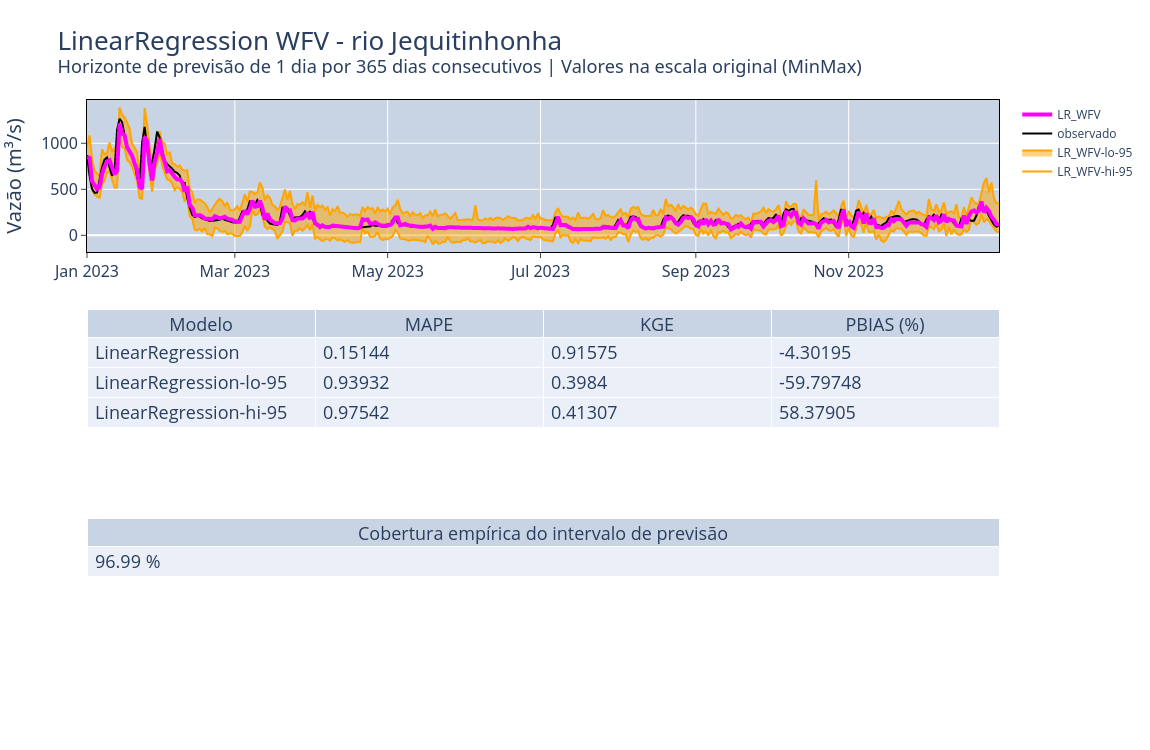
\includegraphics[scale=0.33]{Figuras/jequiti/wfv/LR/LR_WFV_ORIG.png}
	\caption{\textit{Walk-Forward Validation} para o modelo Regressão Linear - LR.\\(fonte: o autor)}
	\label{fig:jequiti_LR_WFV_ORIG}
\end{figure}

%\begin{figure}[!h]
%\centering
%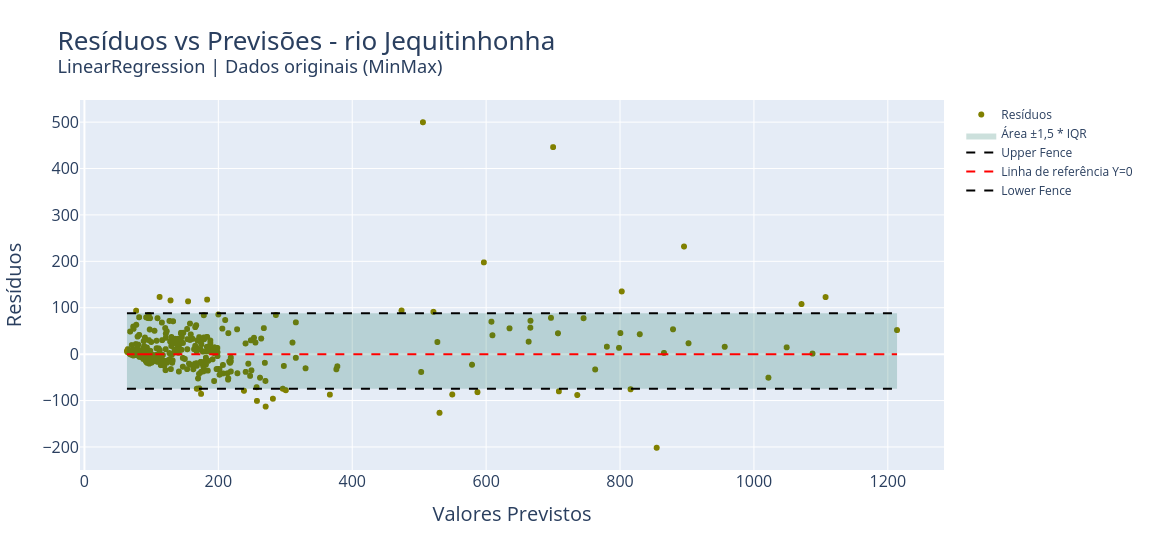
\includegraphics[scale=0.33]{Figuras/jequiti/wfv/LR/LR_WFV_ORIG_RESID_x_PREV.png}
%\caption{Dispersão dos resíduos.\\(fonte: o autor)}
%\label{fig:jequiti_LR_WFV_ORIG_RESID_x_PREV}
%\end{figure}

\begin{figure}[!h]
	\centering
	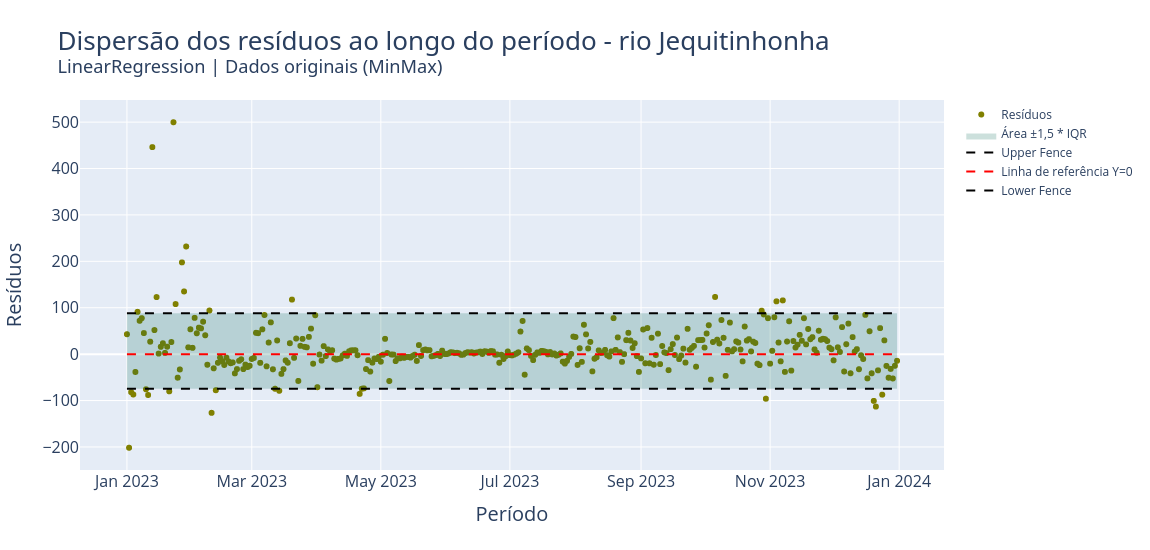
\includegraphics[scale=0.33]{Figuras/jequiti/wfv/LR/LR_WFV_ORIG_RESID_x_TEMPO.png}
	\caption{Dispersão dos resíduos ao longo do ano.\\(fonte: o autor)}
	\label{fig:jequiti_LR_WFV_ORIG_RESID_x_TEMPO}
\end{figure}

\begin{figure}[!h]
	\centering
	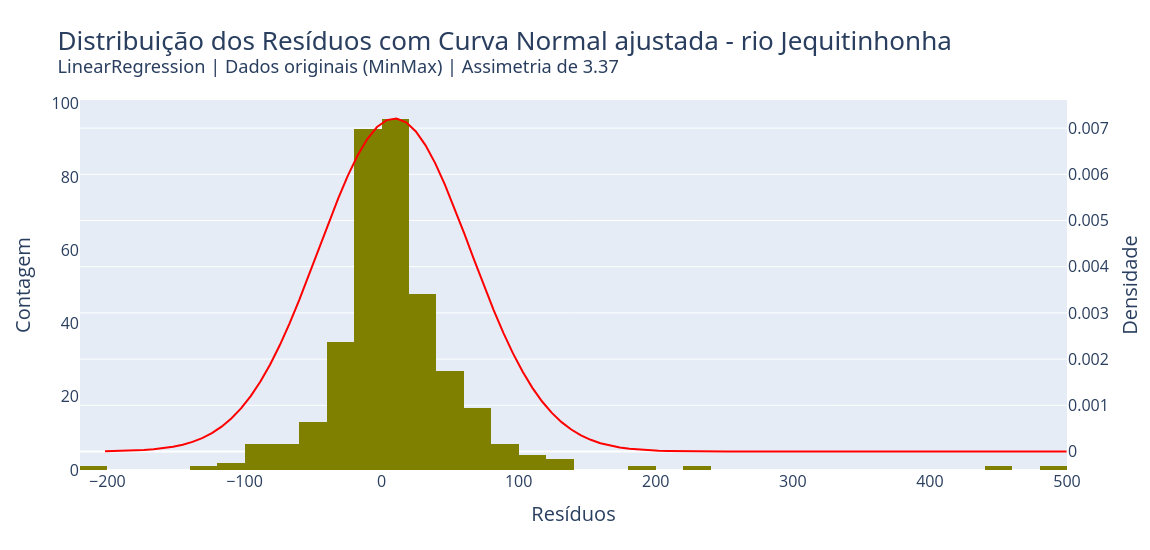
\includegraphics[scale=0.33]{Figuras/jequiti/wfv/LR/LR_WFV_ORIG_RESID_x_CURVA_NORMAL.png}
	\caption{Histograma e curva-normal dos resíduos.\\(fonte: o autor)}
	\label{fig:jequiti_LR_WFV_ORIG_RESID_x_CURVA_NORMAL}
\end{figure}

\begin{figure}[!h]
	\centering
	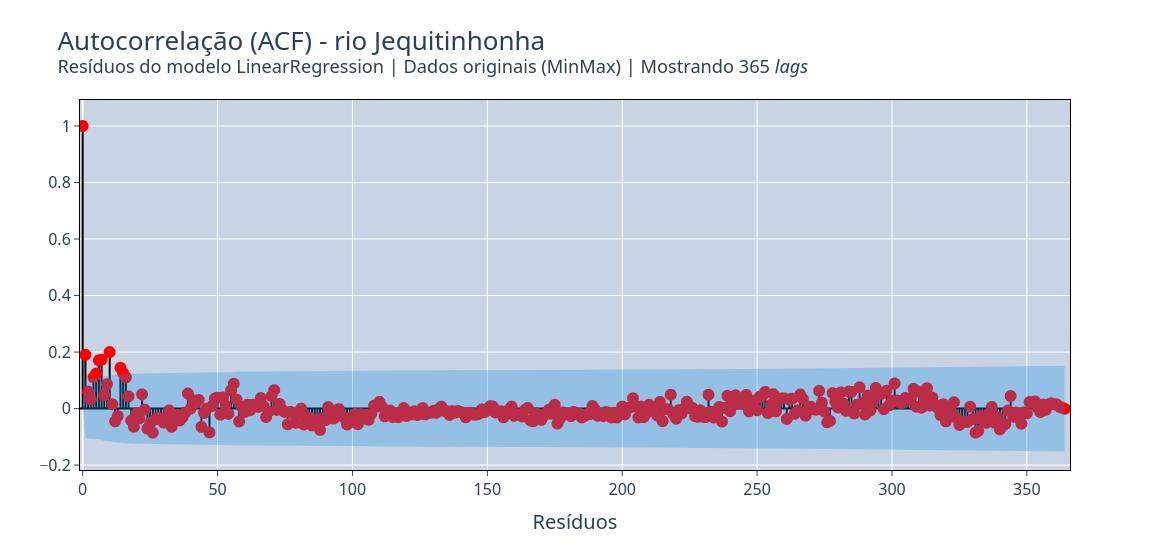
\includegraphics[scale=0.33]{Figuras/jequiti/wfv/LR/LR_WFV_ORIG_RESID_ACF.png}
	\caption{Gráfico ACF dos resíduos.\\(fonte: o autor)}
	\label{fig:jequiti_LR_WFV_ORIG_RESID_ACF}
\end{figure}
\clearpage

Relembrando que a log-transformação lineariza os dados e para o modelo LR ela realmente resultou em melhora dos resultados. Esperava-se que o mesmo pudesse, eventualmente, ocorrer com estes modelos não-lineares, pois simplificaria as relações entre as variáveis. Contudo, aconteceu o oposto. Permanecer com os dados originais, sem nenhum tipo de transformação, foi o que fez ambos, CB e RF, se comportarem melhor.

Veja o comportamento do \textit{walk-forward validation}. Houve melhoras em quase todas as métricas nos dois modelos, exceto para o erro médio percentual, em que ambos tiveram leve piora - $0,133$ para o modelo CB (antes foi $0,130$) e $0,14$ para o RF ($0,12$ antes). É ínfimo, porém não descartável. Mas a KGE, uma métrica mais robusta, melhorou bastante entre o resultado anterior e este resultado em tela. Aplicando os modelos CB e RF nos dados originais, melhorou também o viés sistemático (PBIAS). O modelo CB continuou mostrando tendência de subestimar as previsões mas aqui o modelo RF inverteu, passando a apresentar tendência de superestimar as previsões. A cobertura empírica dos intervalos de previsão melhoraram, sendo o CB quase $2,5\%$ melhor, e o RF melhorou $3\%$ nos cálculos dos intervalos. À respeito dos intervalos de previsão, os modelos mostraram tendência de aumento das faixas ao longo do ano. Diferentemente da análise log-transformada, aqui os modelos parecem ter demostrado incerteza quanto aos erros calculados em eventos anteriores, ainda que no início do ano, para ambos, pareça ter ficado mais estável o cálculo dos intervalos.

\begin{figure}[!h]
	\centering
	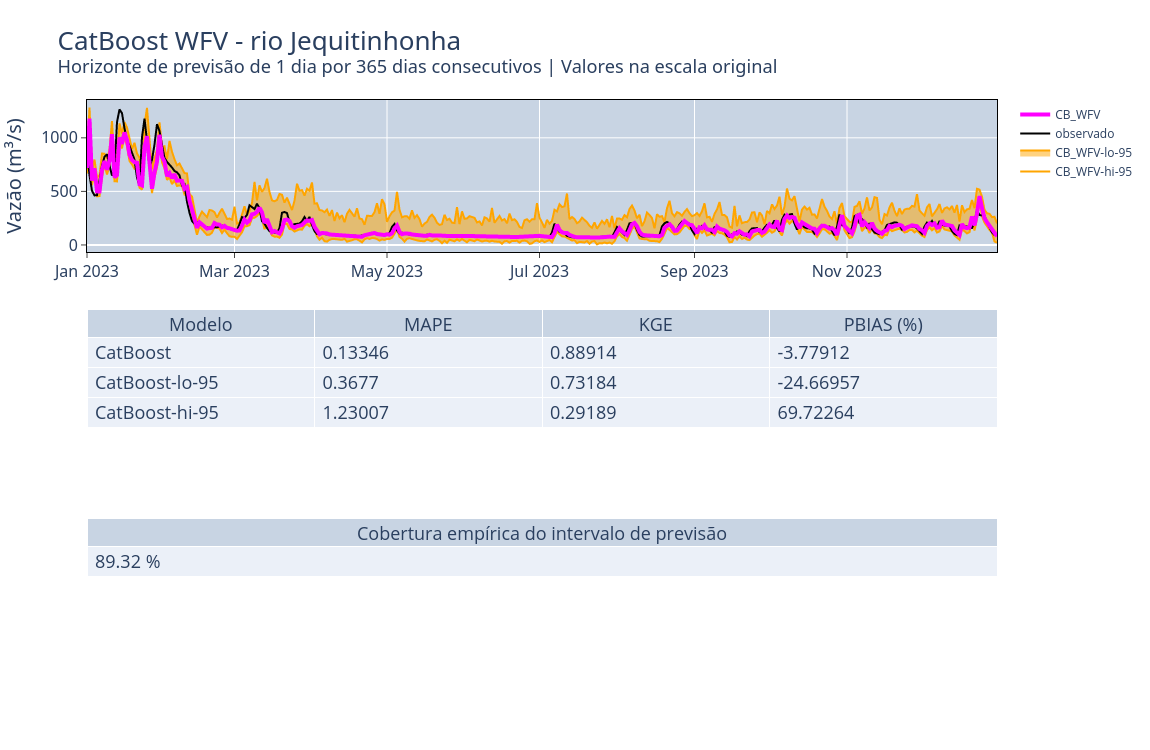
\includegraphics[scale=0.33]{Figuras/jequiti/wfv/CB/CB_WFV_ORIG.png}
	\caption{\textit{Walk-Forward Validation} para o modelo CatBoost - CB.\\(fonte: o autor)}
	\label{fig:jequiti_CB_WFV_ORIG}
\end{figure}

\begin{figure}[!h]
	\centering
	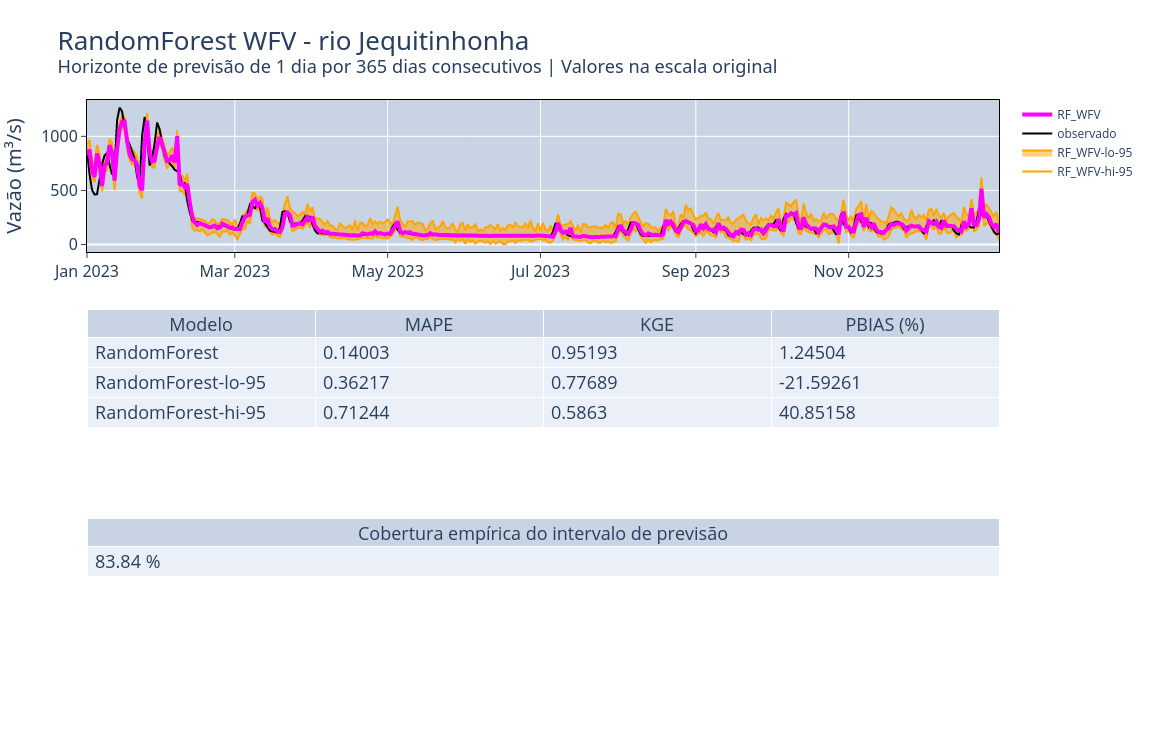
\includegraphics[scale=0.33]{Figuras/jequiti/wfv/RF/RF_WFV_ORIG.png}
	\caption{\textit{Walk-Forward Validation} para o modelo RandomForest - RF.\\(fonte: o autor)}
	\label{fig:jequiti_RF_WFV_ORIG}
\end{figure}
\clearpage

%Observa-se que a maior parte dos resíduos está concentrada em torno da linha de referência $y=0$, o que indica que os modelos CatBoost foram capazes de produzir previsões relativamente boas para a maioria dos dados. Ambos apresentaram também valores extremos, \textit{outliers}, e essa presença pode indicar que os modelos enfrentaram dificuldades em prever corretamente alguns valores mais extremos, resultando em erros maiores para certas previsões. O modelo RF apresenta uma distribuição de resíduos um pouco mais ampla que o CB, com alguns pontos chegando a resíduos superiores a $400$ e abaixo de $-300$.
%
%\begin{figure}[!h]
%\centering
%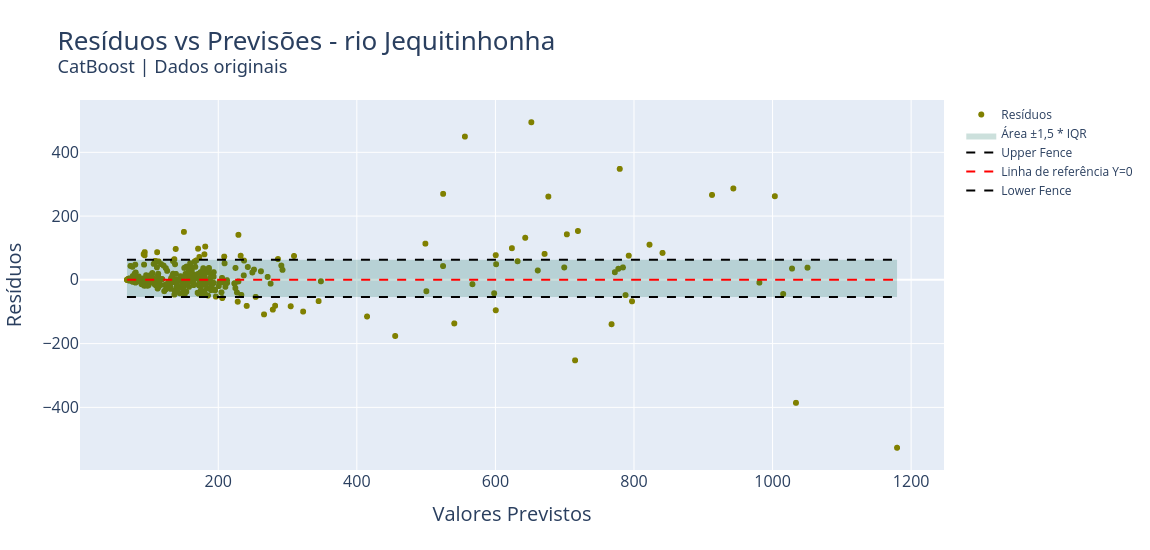
\includegraphics[scale=0.33]{Figuras/jequiti/wfv/CB/CB_WFV_ORIG_RESID_x_PREV.png}
%\caption{Dispersão dos resíduos.\\(fonte: o autor)}
%\label{fig:jequiti_CB_WFV_ORIG_RESID_x_PREV}
%\end{figure}
%
%\begin{figure}[!h]
%\centering
%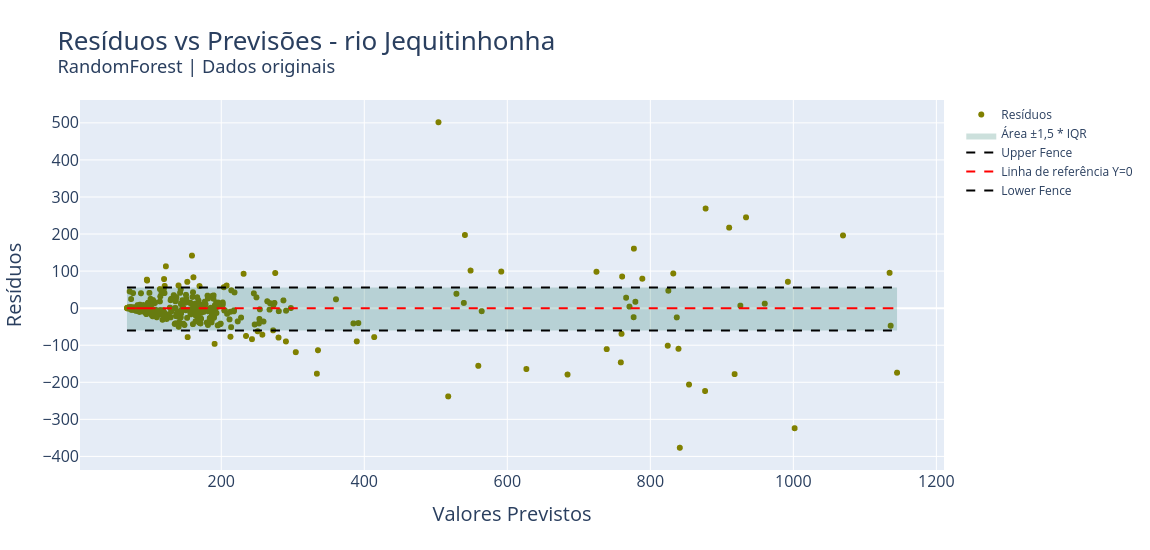
\includegraphics[scale=0.33]{Figuras/jequiti/wfv/RF/RF_WFV_ORIG_RESID_x_PREV.png}
%\caption{Dispersão dos resíduos.\\(fonte: o autor)}
%\label{fig:jequiti_RF_WFV_ORIG_RESID_x_PREV}
%\end{figure}
%\clearpage

A maior parte dos resíduos está concentrada em torno da linha de referência $y=0$, indicando que os modelos mantiveram um desempenho geral estável ao longo do tempo. Porém, há \textit{outliers} significativos no início de $2023$ - valores de resíduos acima de $400$ e abaixo de $-400$ para o CB e acima de $500$ e abaixo de $-300$ para o RF. Esses \textit{outliers} ocorreram em períodos de vazões mais elevadas durante o início do ano, momentos de maiores picos de vazão, indicando que ambos tiveram dificuldades em prever alguns eventos específicos, resultando em erros grandes.

Para o modelo CB, após fevereiro de $2023$, e março para o modelo RF, os resíduos parecem estar melhor distribuídos dentro da área delimitada pelas faixas, com menos \textit{outliers}, sugerindo que os modelos ajustaram-se melhor aos dados ao longo do tempo e permaneceram estáveis.

Em geral, ambos os modelos apresentaram um padrão de melhora ao longo do ano, com resíduos mais bem distribuídos após o primeiro trimestre de $2023$. No entanto, os \textit{outliers} iniciais indicam que os modelos podem ter dificuldades com eventos específicos de sazonalidade ou anomalias no início do ano. O CB parece ter uma leve vantagem em termos de previsões mais consistentes ao longo do tempo, com valores menos extremos. Houve uma prevalência de $85,75\%$ dos resíduos dentro da área sombreada do gráfico \ref{fig:jequiti_CB_WFV_ORIG_RESID_x_TEMPO}, ao passo que o modelo RF obteve $84,11\%$ de prevalência - gráfico \ref{fig:jequiti_RF_WFV_ORIG_RESID_x_TEMPO}. Ajustes de hiperparâmetros podem ajudar os modelos nos períodos mais desafiadores do ano, como no início do ano, ou adição de componentes de tendência e sazonalidade localizada.

\begin{figure}[!h]
	\centering
	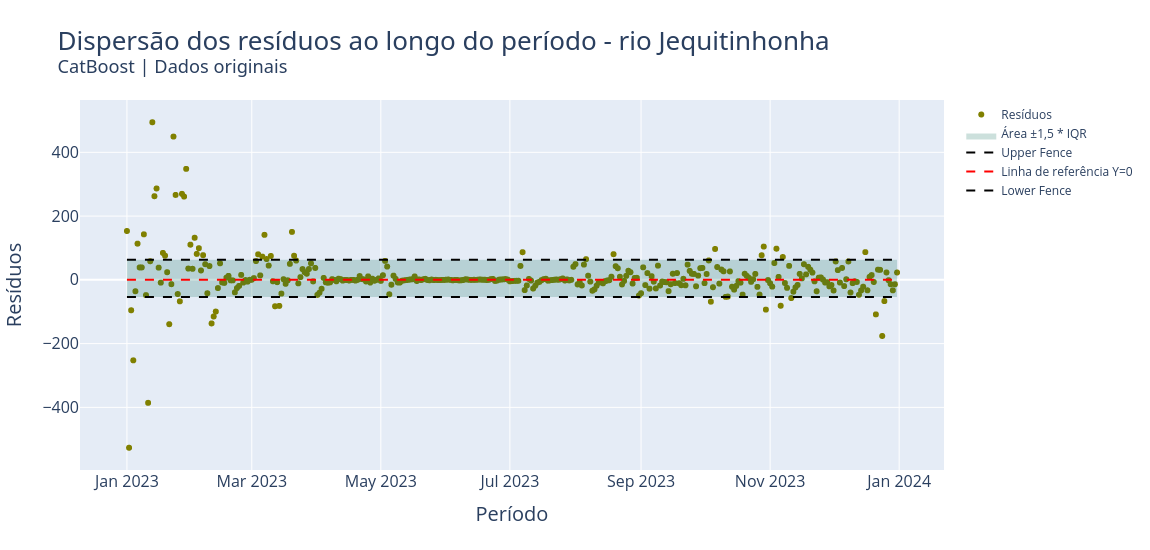
\includegraphics[scale=0.33]{Figuras/jequiti/wfv/CB/CB_WFV_ORIG_RESID_x_TEMPO.png}
	\caption{Dispersão dos resíduos ao longo do ano.\\(fonte: o autor)}
	\label{fig:jequiti_CB_WFV_ORIG_RESID_x_TEMPO}
\end{figure}

\begin{figure}[!h]
	\centering
	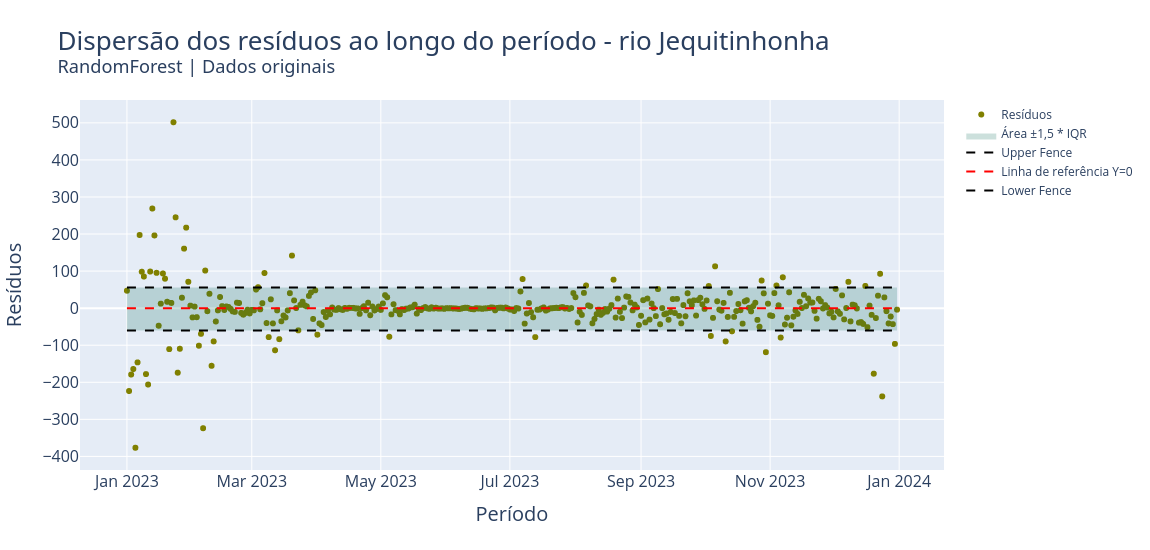
\includegraphics[scale=0.33]{Figuras/jequiti/wfv/RF/RF_WFV_ORIG_RESID_x_TEMPO.png}
	\caption{Dispersão dos resíduos ao longo do ano.\\(fonte: o autor)}
	\label{fig:jequiti_RF_WFV_ORIG_RESID_x_TEMPO}
\end{figure}
\clearpage

A distribuição dos resíduos do modelo CB - figura \ref{fig:jequiti_CB_WFV_ORIG_RESID_x_CURVA_NORMAL} - apresenta uma assimetria positiva de $0,66$, o que indica que a cauda direita da distribuição é mais longa que a esquerda. A presença de resíduos elevados tanto na cauda direita - acima de $200$ - quanto na cauda esquerda - abaixo de $-100$ - indica que o modelo teve dificuldades em prever com precisão alguns valores mais extremos. A curva normal ajustada em vermelho não se adequa perfeitamente à distribuição observada, especialmente nas caudas, deixando claro que a distribuição dos resíduos não é perfeitamente normal. Esse comportamento é esperado, dado o valor da assimetria. Contudo, a maior parte dos resíduos está concentrada em torno de $y=0$, com uma contagem elevada próxima a $0$. Isso é um bom sinal, pois sugere que o modelo fez previsões razoavelmente precisas para a maior parte das observações.

A distribuição dos resíduos do modelo RF - figura \ref{fig:jequiti_RF_WFV_ORIG_RESID_x_CURVA_NORMAL} - apresenta uma assimetria positiva de $0,49$, indicando que a cauda direita é um pouco mais longa, mas a assimetria é menos pronunciada do que no modelo CB. A curva normal ajustada se aproxima mais da distribuição observada do que no gráfico do CB, o que sugere que os resíduos do RF seguem uma distribuição mais próxima de uma distribuição normal, apesar da pequena assimetria positiva. Assim como no gráfico do CB, a maior parte dos resíduos está concentrada em torno de $0$, com a maioria das previsões sendo razoavelmente precisas, porém, o modelo RF apresenta um adensamento ligeiramente mais equilibrada.

O RF tem um comportamento de resíduos mais próximo de uma distribuição normal, caracterizando-o como mais estável e robusto em termos de previsões para a maioria dos dados. O CB mostrou sensibilidade a eventos extremos, com uma assimetria maior, indicando que o modelo enfrenta dificuldades em capturar corretamente estes valores mais extremos, resultando em erros maiores. Mas em geral, ambos os modelos apresentaram uma boa concentração de resíduos em torno de $0$ - praticamente indistinguível -, mostrando que a maioria das previsões está correta.

\begin{figure}[!h]
\centering
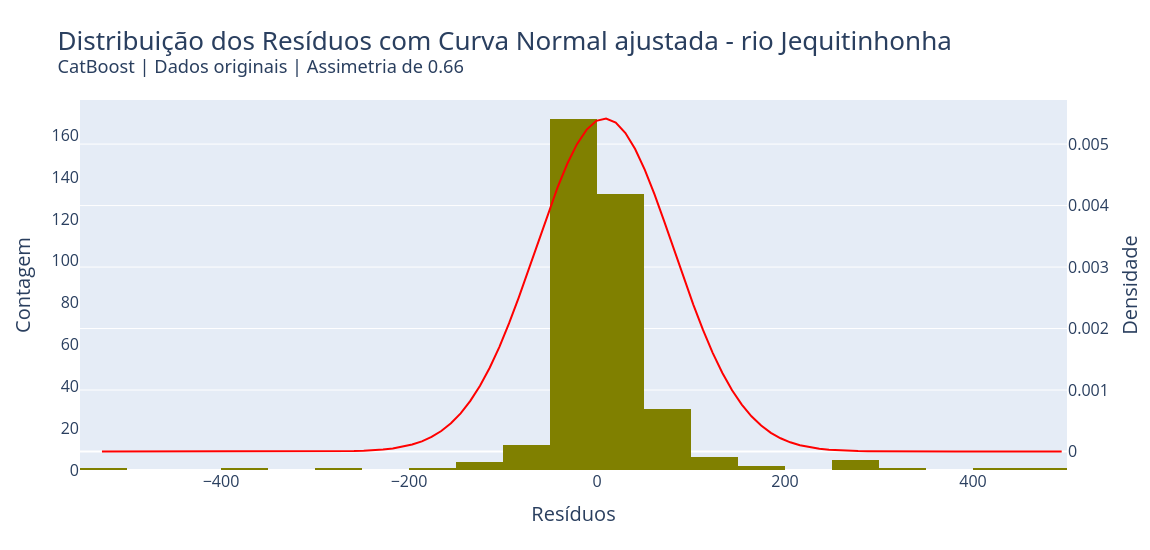
\includegraphics[scale=0.33]{Figuras/jequiti/wfv/CB/CB_WFV_ORIG_RESID_x_CURVA_NORMAL.png}
\caption{Histograma e curva-normal dos resíduos.\\(fonte: o autor)}
\label{fig:jequiti_CB_WFV_ORIG_RESID_x_CURVA_NORMAL}
\end{figure}

\begin{figure}[!h]
\centering
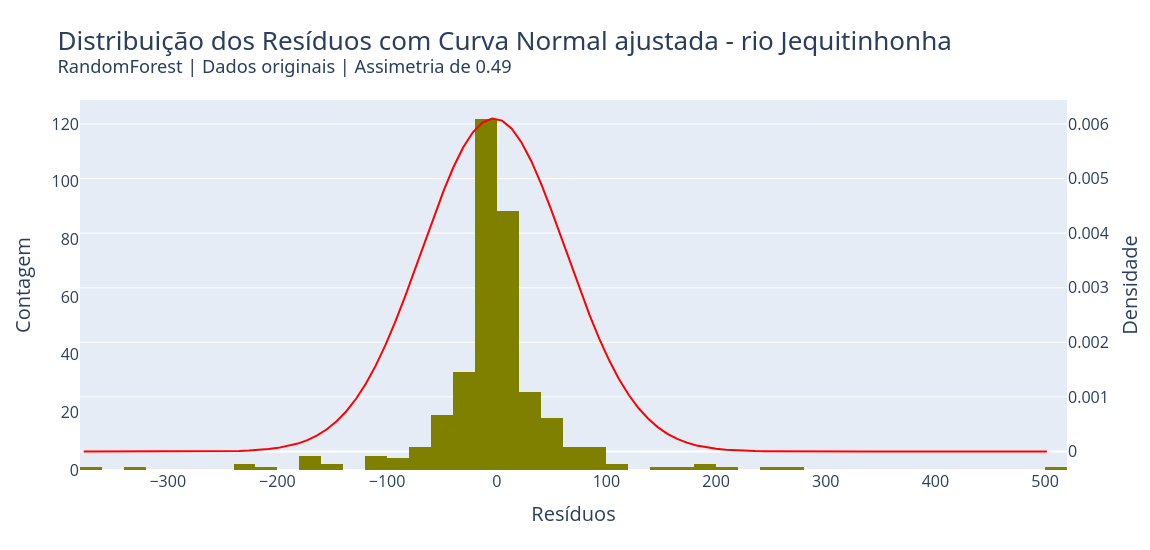
\includegraphics[scale=0.33]{Figuras/jequiti/wfv/RF/RF_WFV_ORIG_RESID_x_CURVA_NORMAL.png}
\caption{Histograma e curva-normal dos resíduos.\\(fonte: o autor)}
\label{fig:jequiti_RF_WFV_ORIG_RESID_x_CURVA_NORMAL}
\end{figure}
\clearpage

Nas primeiras \textit{lags}, há autocorrelações significativas que ultrapassam a faixa de confiança, especialmente nas primeiras $15$ \textit{lags}. Para curtos intervalos de tempo, os resíduos do modelo CB estão correlacionados - figura \ref{fig:jequiti_CB_WFV_ORIG_RESID_ACF}. A presença dessas correlações positivas nas primeiros \textit{lags} pode sugerir que há padrões temporais de curto prazo nos dados que o modelo CB não capturou adequadamente. No entanto, após essa \textit{lag} $15$, as autocorrelações caem para valores dentro da faixa de confiança de $95\%$ e permanecem próximas de $0$. Isso mostra que, para intervalos maiores, os resíduos não apresentam correlação significativa, o que é um sinal positivo de que, em termos de longo prazo, o modelo está capturando a variabilidade dos dados de forma satisfatória.

Assim como no gráfico do CB, o modelo RF também apresenta autocorrelações significativas nas primeiras \textit{lags}, até perto de $20$ \textit{lags} - figura \ref{fig:jequiti_RF_WFV_ORIG_RESID_ACF}. Houve um comportamento levemente pior aqui - levou mais $5$ \textit{lags} para estabilizar - neste modelo do que em relação ao CB, indicando, semelhantemente, uma dependência temporal de curto prazo que o modelo RF não capturou completamente, resultando em resíduos correlacionados nas primeiras \textit{lags}. A partir da \textit{lag} $20$, as autocorrelações do RF caem para dentro da faixa de confiança e permanecem próximas de $0$, assim como no modelo CB, indicando que, para previsões de longo prazo, o modelo RF também está capturando bem a estrutura dos dados e os resíduos se comportam de maneira aleatória.

Ambos os modelos CB e RF apresentam autocorrelações significativas nas primeiras \textit{lags}, denotando que nenhum modelo conseguiu capturar completamente a dependência temporal de curto prazo nos dados. No entanto, o CB teve uma dispersão um pouco menor de correlações significativas em comparação com o RF, o que indica um desempenho ligeiramente melhor no curto prazo.

Para \textit{lags} maiores (acima de $20$), tanto o CB quanto o RF apresentaram resíduos que se comportaram de maneira aleatória, com autocorrelações dentro da faixa de confiança e próximas de $0$. Considernado as previsões de longo prazo, ambos os modelos estão funcionando de forma satisfatória e não apresentaram padrões remanescentes nos resíduos.

\begin{figure}[!h]
	\centering
	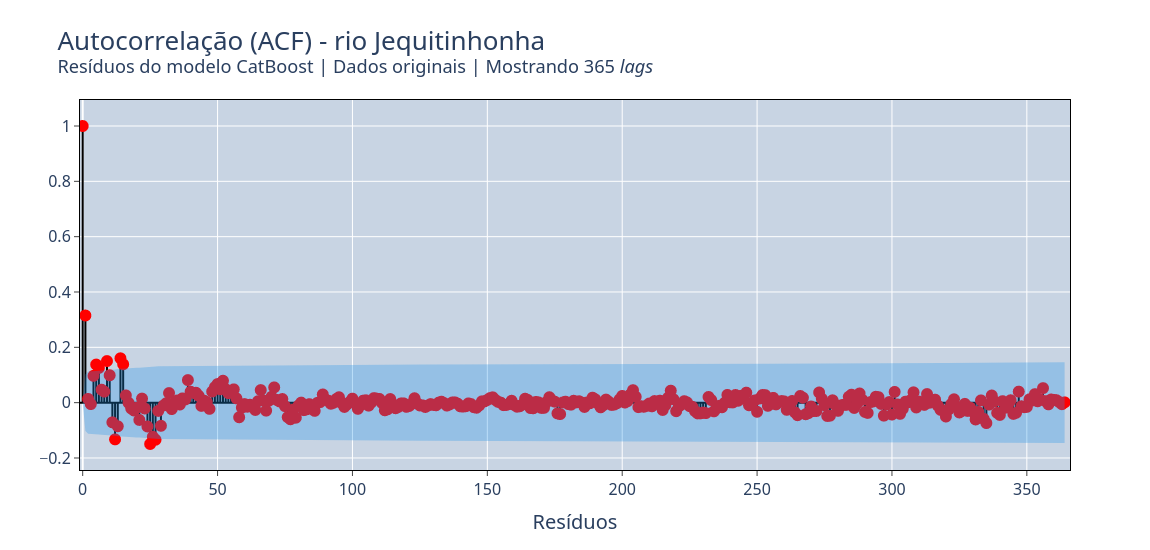
\includegraphics[scale=0.33]{Figuras/jequiti/wfv/CB/CB_WFV_ORIG_RESID_ACF.png}
	\caption{Gráfico ACF dos resíduos.\\(fonte: o autor)}
	\label{fig:jequiti_CB_WFV_ORIG_RESID_ACF}
\end{figure}

\begin{figure}[!h]
	\centering
	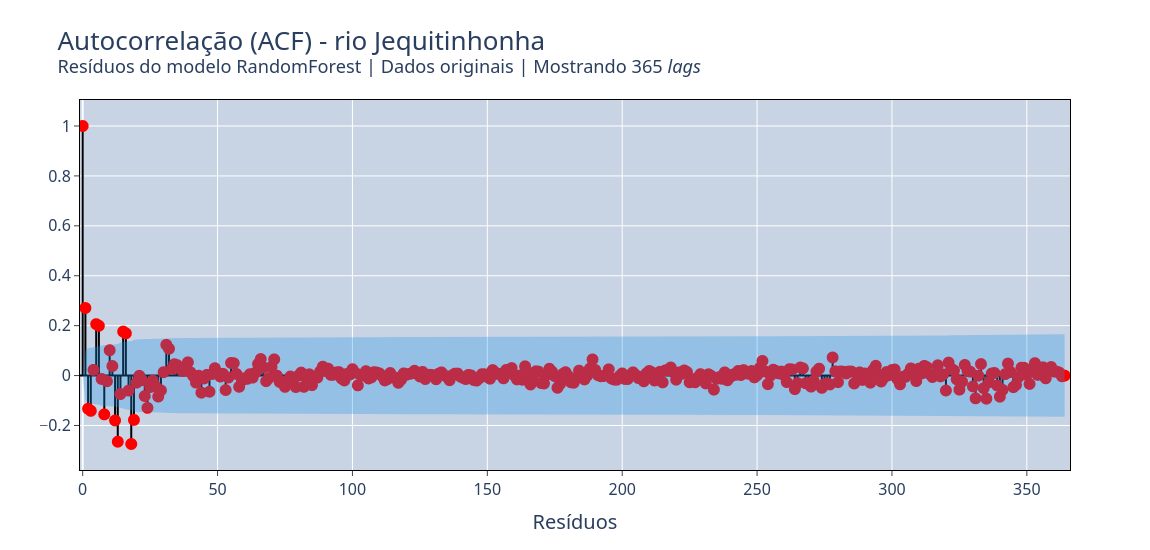
\includegraphics[scale=0.33]{Figuras/jequiti/wfv/RF/RF_WFV_ORIG_RESID_ACF.png}
	\caption{Gráfico ACF dos resíduos.\\(fonte: o autor)}
	\label{fig:jequiti_RF_WFV_ORIG_RESID_ACF}
\end{figure}
\clearpage

Para o rio Jequitinhonha a análise termina aqui. Aplicar a log-transformação melhorou o resultado do modelo LR de quando não foi aplicada essa transformação, e os modelos CB e RF (não-lineares) foram melhores quando os dados não foram transformados. Aqui, para este rio, foi este o resultado, mais adiante será visto para os demais rios.

Uma coisa que precisa ficar claro aqui: \underline{só serão discutidos para os outros rios os melhores resultados}. Para o Jequitinhonha foi mostrada toda linha de trabalho para que ficasse claro que toda comparação foi realizada entre resultados log-transformados e não transformados, tudo foi estudado e analisado. Mas pelo bem da concisão - e deve ter ficado evidente as voltas dadas no texto mostrando exatamente cada resultado - todo resultado não mostrado neste capítulo será colocado em um apêndice para que o leitor e a leitora possam averiguar a corretude do trabalho. E não será mais incluída a análise para o modelo SeasonalNaive.

Adiante.

\subsection{Rio Doce}

Os resultados para o rio Doce apresentaram-se muito bons, considerando-se todas as métricas do trabalho. Isso possivelmente se deve à qualidade dos dados de treinamento, em que não foi preciso preencher tantos dados faltantes de vazão. Relembre: de $4017$ registros, apenas $3$ faltavam.

O modelo CB apresentou um desempenho muito bom, com KGE de $0,89$ sugerindo alta correlação entre os valores previstos e observados. Quando se considera a MAPE, foi a mais baixa dentre os três modelos, contudo, mesmo assim, indica uma precisão elevada nas previsões médias, o que demonstra robustez do modelo. A PBIAS de $-3.73\%$ mostra um leve viés geral para subestimar as previsões, e a cobertura empírica de $91,23\%$ indica que o intervalo de previsão capturou bem a variabilidade dos dados observados.

O gráfico \ref{fig:doce_CB_WFV_ORIG} revela ainda que o modelo acompanha bem os picos de vazão e que os intervalos de previsão foram particularmente estreitos quando no período de vazões elevadas e relativamente amplos nos períodos de menores vazões, podendo indicar que as medições de precipitação nos períodos chuvosos conferem mais precisão ao comportamento médio do modelo. Em outras palavras: o modelo fica ``otimista'' quando os dados de chuva não estão zerados e possui mais informações, o que ocorre nos períodos de outono e inverno. Tanto que nestes períodos mencionados, quando há uma profusão de valores $0$ na precipitação, os intervalos de previsão ficaram amplos, o que denota a tentativa do modelo de ``acertar'' a medida. Comportamento este que o modelo RF também apresentou em relação aos intervalos de previsão - visto em \ref{fig:doce_RF_WFV_ORIG}. A cobertura empírica dos intervalos de previsão de ambos os modelos ficaram próximas, com uma leve vantagem para o modelo CB - o modelo RF obteve $88,77\%$.

O modelo LR, mesmo sendo um modelo simples, apresentou um desempenho notável, com uma MAPE ligeiramente maior, de $0,084$, do que a do CB, mas ainda assim baixa. A KGE foi a maior dos três modelos, alcançando $0,94$, mostrando uma ótima correlação e menor erro de variância entre os valores observados e os previstos. A PBIAS de $-2,75\%$ sugere um viés de subestimação, sendo o ``caminho do meio'' entre os modelos. A cobertura empírica de $96,71\%$ indica que o intervalo de previsão captura quase a totalidade da variabilidade dos dados observados - visível no gráfico \ref{fig:doce_LR_WFV_LOG}. O gráfico também mostra que o LR também consegue capturar os picos de vazão de forma eficaz, com intervalos de previsão mais estreitos ao longo do ano se comparados ao CB e ao RF, porém mais amplos no período inicial do ano.

O modelo RF também teve um bom desempenho, com uma MAPE intermediária entre os outros dois modelos e uma KGE de $0,93$, ficando muito próxima a do LR. A PBIAS de $-1,44\%$ indica o menor viés de subestimação entre os três modelos, no entanto, a cobertura empírica foi a menor, com $88,77\%$, sugerindo que os intervalos de previsão não abrangem tanto a variabilidade observada quanto nos outros modelos. Isso é perceptível principalmente no início da série, nos meses de janeiro, fevereiro e março, ainda que tenha captado bem os picos de vazão, um comportamento semelhante ao CB em termos de previsões.

Em termos de precisão média (MAPE), o CB apresentou o melhor desempenho - valor de $0,082$ -, seguido de perto por RF - valor de $0,083$ - e LR - MAPE de $0,084$. A diferença foi muito pequena, na casa de $10^{-3}$, mostrando que todos os modelos tiveram alta precisão. Analisando a KGE - a mais complexa das métricas, que avalia a correlação, a variabilidade e o viés -, o modelo LR foi o melhor nesse critério, seguido por RF e CB. Isso sugere que, apesar de ser um modelo linear, a regressão conseguiu capturar bem a dinâmica não-linear das vazões do rio. Mas, novamente, os valores ficaram muito próximos, não havendo grande discrepância entre as medições.

%\begin{itemize}
%	\item No geral, todos os três modelos apresentam bons resultados, mas com características específicas:
%	\begin{itemize}
%		\item O modelo CB saiu-se ligeiramente melhor em precisão - MAPE -, mas com um viés de subestimação mais acentuado;
%		\item O modelo LR surpreendentemente teve o melhor desempenho na KGE, um viés mediano e a melhor cobertura empírica; e
%		\item O modelo RF mostrou-se competitivo em precisão e viés, porém, com uma menor cobertura empírica, o que sugere que os intervalos de previsão são menos eficazes para capturar a incerteza nas previsões quando comparado aos demais modelos.
%	\end{itemize}
%\end{itemize}

\begin{figure}[!h]
	\centering
	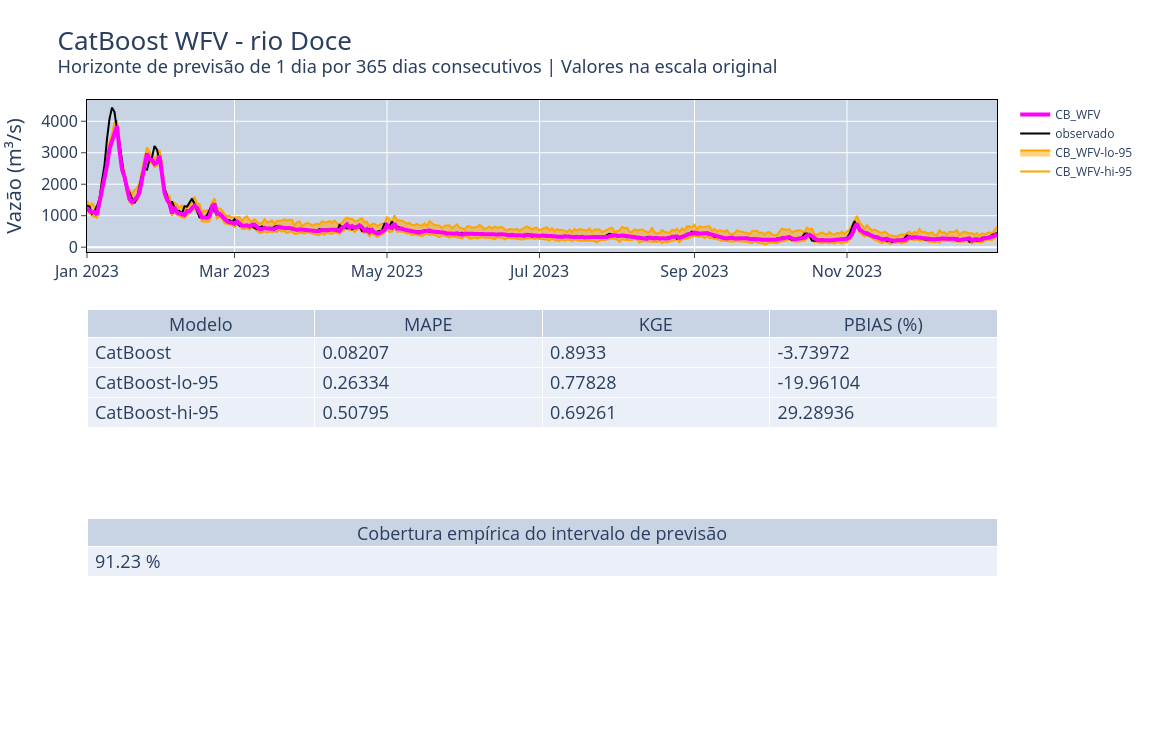
\includegraphics[scale=0.33]{Figuras/rio_doce/wfv/CB/CB_WFV_ORIG.png}
	\caption{\textit{Walk-Forward Validation} para o modelo CatBoost - CB.\\(fonte: o autor)}
	\label{fig:doce_CB_WFV_ORIG}
\end{figure}

\begin{figure}[!h]
	\centering
	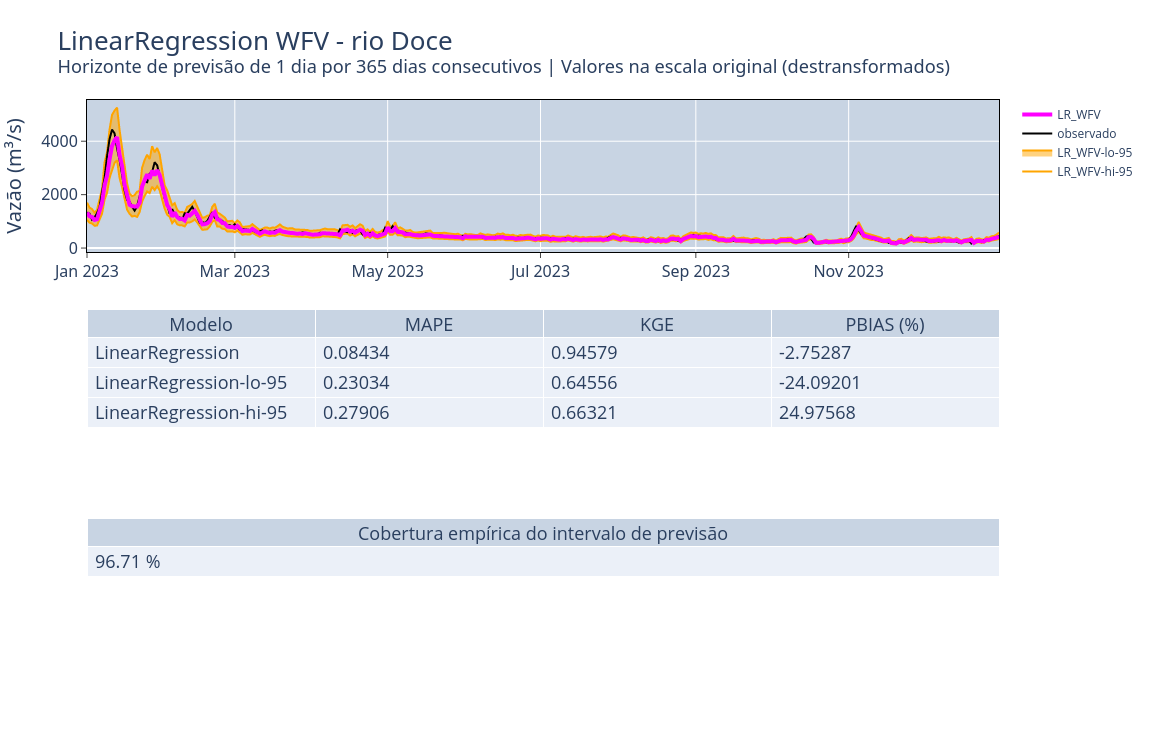
\includegraphics[scale=0.33]{Figuras/rio_doce/wfv/LR/LR_WFV_LOG.png}
	\caption{\textit{Walk-Forward Validation} para o modelo LinearRegression - LR.\\(fonte: o autor)}
	\label{fig:doce_LR_WFV_LOG}
\end{figure}

\begin{figure}[!h]
	\centering
	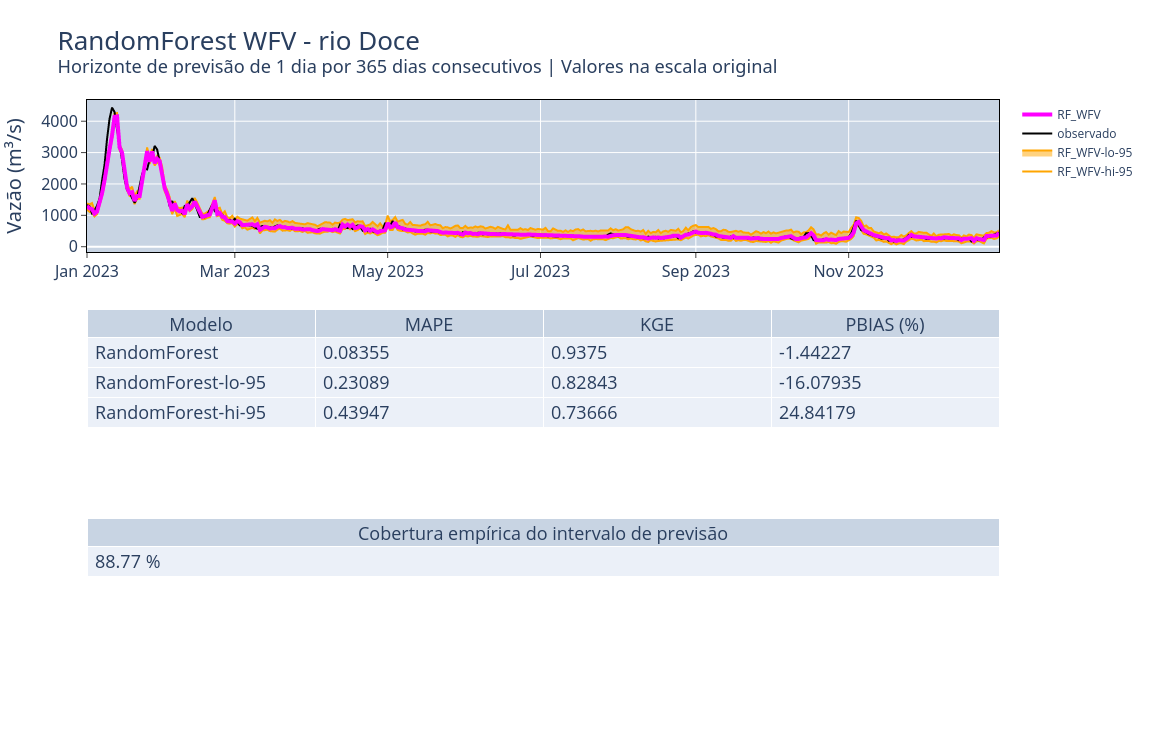
\includegraphics[scale=0.33]{Figuras/rio_doce/wfv/RF/RF_WFV_ORIG.png}
	\caption{\textit{Walk-Forward Validation} para o modelo RandomForest - RF.\\(fonte: o autor)}
	\label{fig:doce_RF_WFV_ORIG}
\end{figure}
\clearpage

%O gráfico \ref{fig:doce_CB_WFV_ORIG_RESID_x_PREV} do modelo CB mostra uma concentração de resíduos em torno de $0$ para previsões de até aproximadamente $700 m^3/s$, o que indica que o modelo está prevendo bem para valores moderados de vazão. No entanto, à medida que os valores previstos aumentam, os resíduos começam a se espalhar mais, evidenciando que o modelo tem dificuldade em capturar picos de vazão mais elevados.
%
%Existem alguns resíduos que excedem os limites de $\pm 1,5 \times IQR$, especialmente para previsões mais altas, com diversos resíduos acima de $200$ o que mostra a presença de \textit{outliers} em picos de vazão. E não parece haver uma tendência clara nos resíduos, o que é positivo, pois significa que o modelo não está sistematicamente superestimando ou subestimando em uma faixa específica de valores previstos.

%Para o LR, observa-se no gráfico \ref{fig:doce_LR_WFV_LOG_RESID_x_PREV} um comportamento semelhante ao do CB no que se refere à concentração de resíduos em torno de $0$ para valores previstos mais baixos. Contudo, a dispersão dos resíduos é ligeiramente maior para previsões acima de $1000 m^3/s$, indicando uma leve perda de precisão em valores mais altos.

%O modelo LR também mostra alguns \textit{outliers} em valores previstos mais altos, especialmente entre $2500$ e $4000 m^3/s$. Isso é esperado, dado que a regressão linear pode ter dificuldades em capturar não-linearidades e picos extremos de vazão. Repete-se aqui o mesmo comportamento do CB e não há uma tendência evidente, o que significa que o modelo está relativamente bem ajustado, mas com uma dispersão maior à medida que os valores previstos aumentam.
%
%O RF apresentou um padrão semelhante aos dos modelos anteriores. A concentração dos resíduos em torno de $0$ para previsões menores também está presente, mas há uma maior dispersão dos resíduos para previsões acima de $1000 m^3/s$. Isso pode indicar que, assim como os outros modelos, o RF apresentou dificuldade em capturar corretamente alguns picos mais altos de vazão. Vale salientar que todos os modelos apresentaram viés geral sistemático de subestimação das previsões
%
%Notam-se \textit{outliers} para valores previstos mais altos, com resíduos que variam de $300$ a mais de $1000$ para previsões maiores que $2500 m^3/s$. Esses \textit{outliers} são mais pronunciados que nos outros dois modelos. Estes valores elevados indicando outliers denotam que este modelo, bem como os outros anteriores, perde precisão em alguns valores de pico de vazão observados. Por fim, não houve uma tendência clara nos resíduos.
%
%Em geral, todos os três modelos apresentam uma concentração de resíduos razoavelmente próxima de $0$ para valores de vazão previstos abaixo de $1000 m^3/s$ - prevalência de $87,4\%$ para resíduos dos modelos CB e RF e de $88,22\%$ para LR dentro da faixa $\pm 1,5 \times IQR$ -, sugerindo que eles conseguem modelar bem as vazões mais comuns e de baixa intensidade. À medida que os valores previstos aumentam, todos os modelos mostram uma dispersão crescente nos resíduos, com picos de vazão sendo mais difíceis de prever corretamente. Contudo, o RF parece ter a maior dispersão, seguido por LR, enquanto que o CB apresentou uma dispersão ligeiramente menor, embora ainda presente.
%
%Os três modelos possuem \textit{outliers}, especialmente em previsões mais altas, mostrando que isso é um desafio em dados de vazão de rios, que apresentam picos esporádicos. O RF tem os \textit{outliers} mais extremos, seguidos por LR e, por fim, CB. A crescente dispersão dos resíduos em valores previstos mais altos sugere que \underline{todos os modelos} enfrentaram desafios em prever valores de vazão muito elevados, ainda que tenham acompanhado os picos de vazão.

%\begin{figure}[!h]
%\centering
%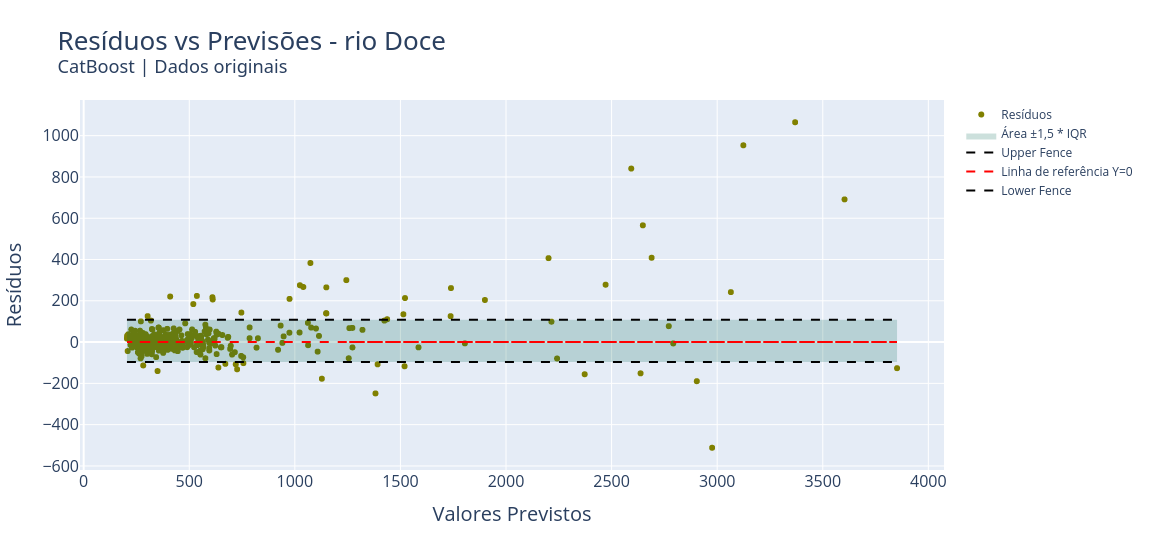
\includegraphics[scale=0.33]{Figuras/rio_doce/wfv/CB/CB_WFV_ORIG_RESID_x_PREV.png}
%\caption{Dispersão dos resíduos.\\(fonte: o autor)}
%\label{fig:doce_CB_WFV_ORIG_RESID_x_PREV}
%\end{figure}
%
%\begin{figure}[!h]
%\centering
%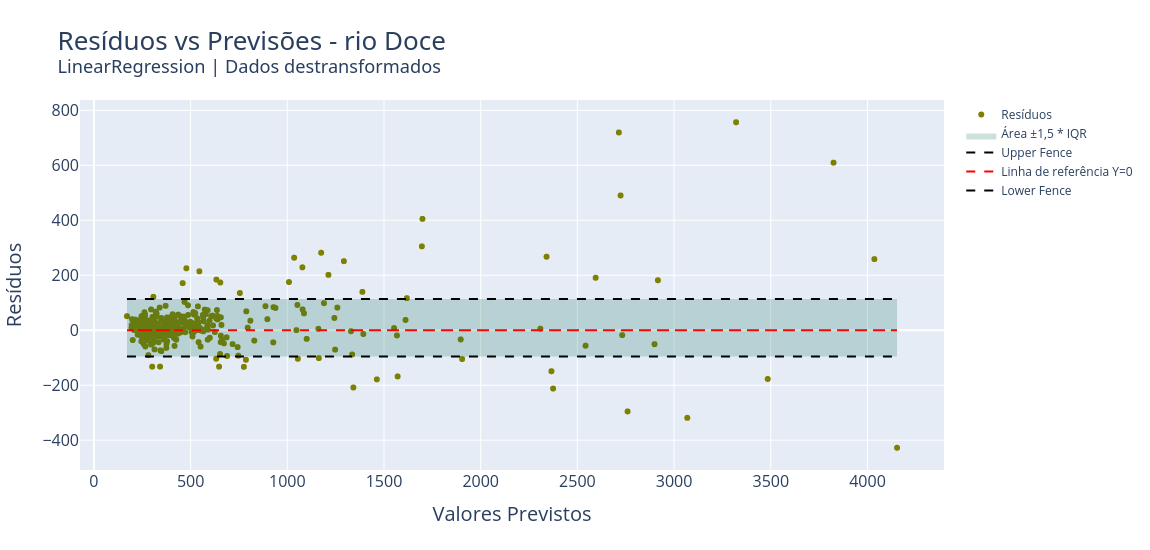
\includegraphics[scale=0.33]{Figuras/rio_doce/wfv/LR/LR_WFV_LOG_RESID_x_PREV.png}
%\caption{Dispersão dos resíduos.\\(fonte: o autor)}
%\label{fig:doce_LR_WFV_LOG_RESID_x_PREV}
%\end{figure}
%
%\begin{figure}[!h]
%\centering
%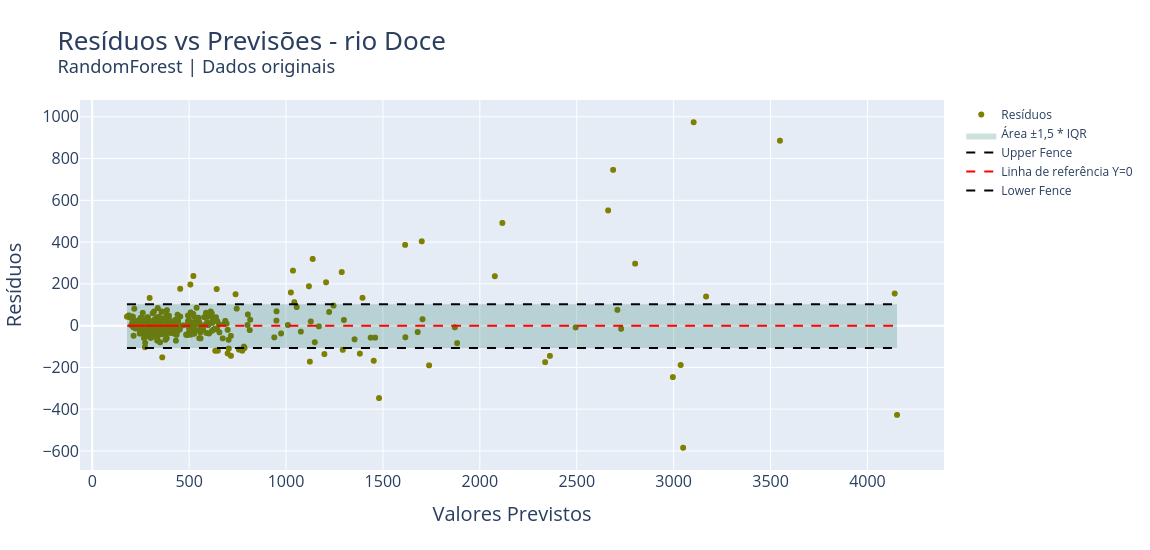
\includegraphics[scale=0.33]{Figuras/rio_doce/wfv/RF/RF_WFV_ORIG_RESID_x_PREV.png}
%\caption{Dispersão dos resíduos.\\(fonte: o autor)}
%\label{fig:doce_RF_WFV_ORIG_RESID_x_PREV}
%\end{figure}
%\clearpage

No gráfico \ref{fig:doce_CB_WFV_ORIG_RESID_x_TEMPO} é possível observar que no início do período - janeiro e fevereiro de $2023$ -, os resíduos estão mais dispersos, com muitos valores além dos limites $\pm 1,5 \times IQR$, tanto na parte superior quanto na inferior. Isso denota que o modelo teve dificuldades em prever corretamente durante essa fase inicial do ano, que pode estar associada a picos de vazão ou condições hidrológicas atípicas. Após março de $2023$, os resíduos começam a se concentrar dentro dos intervalos, de onde se conclui que o modelo se estabilizou e começou a prever com mais precisão, com menos erros extremos, ou seja, o CB foi capaz de capturar bem o padrão de vazões ao longo do ano, exceto em eventos de pico no início.

Da mesma forma que o CB, o modelo LR mostra uma maior dispersão dos resíduos no início do período, particularmente nos meses de janeiro e fevereiro de $2023$ - figura \ref{fig:doce_LR_WFV_LOG_RESID_x_TEMPO}. A partir de março de $2023$ os resíduos do LR também se tornam mais estáveis e permanecem concentrados dentro da área sombreada, indicando uma melhor performance com o passar do tempo e em períodos de amenidades nas vazões.

E, finalmente, o modelo RF - figura \ref{fig:doce_RF_WFV_ORIG_RESID_x_TEMPO}. O comportamento dos resíduos do RF ao longo do tempo é similar ao dos outros dois modelos anteriores. Há uma maior dispersão no início do ano (janeiro e fevereiro de $2023$), mas a partir de março os resíduos se tornam mais estáveis, com a maioria dos valores dentro da aŕea destacada. Indica que o RF também teve dificuldades em capturar os eventos extremos no início do ano e que também apresentou bom desempenho para o restante do período.

Os três modelos enfrentaram desafios semelhantes durante o período inicial do ano - janeiro e fevereiro -, comportamento quase indistinguível entre eles, mas todos estabilizaram a partir de março, sem que tenha um modelo que realmente se destaque frente aos demais. O comportamento dos resíduos ao longo do tempo indica que, para períodos com picos sazonais, pode ser necessário um refinamento adicional nos modelos ou mesmo refinamento nos dados de entrada para melhor capturar estes eventos.

\begin{figure}[!h]
	\centering
	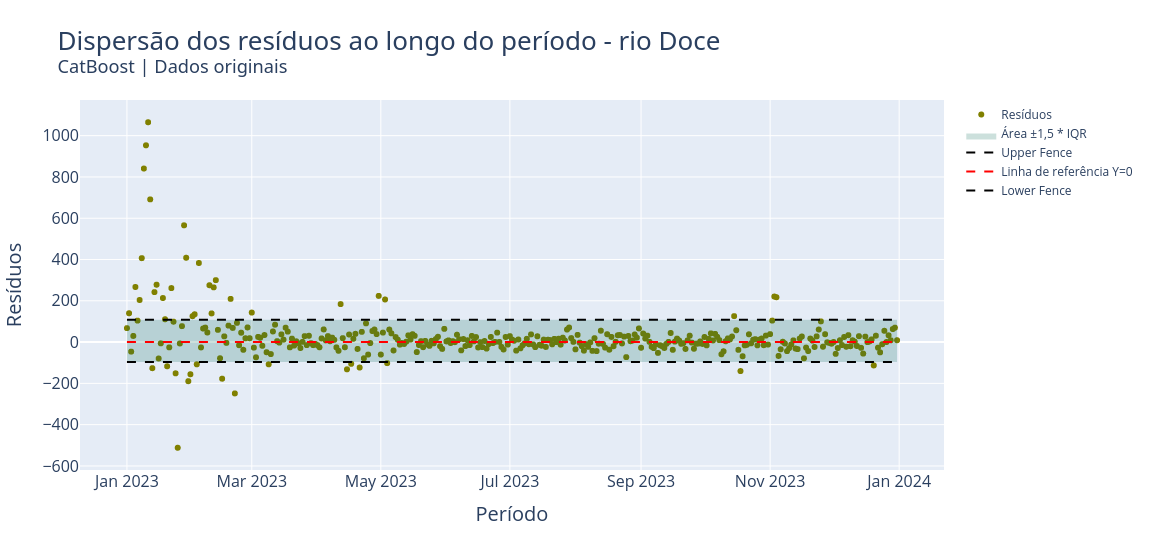
\includegraphics[scale=0.33]{Figuras/rio_doce/wfv/CB/CB_WFV_ORIG_RESID_x_TEMPO.png}
	\caption{Dispersão dos resíduos ao longo do ano.\\(fonte: o autor)}
	\label{fig:doce_CB_WFV_ORIG_RESID_x_TEMPO}
\end{figure}

\begin{figure}[!h]
	\centering
	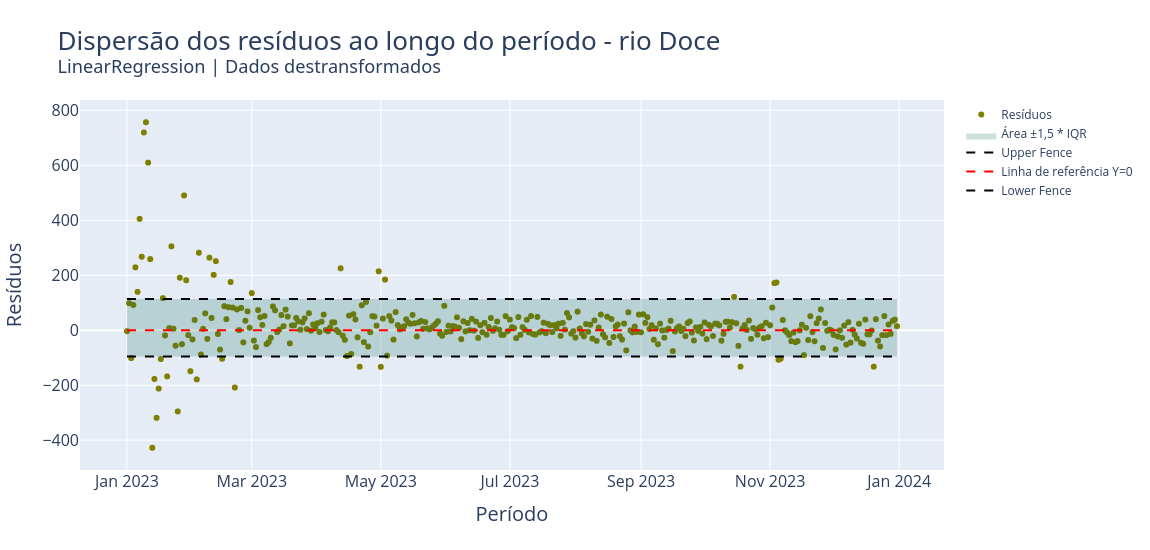
\includegraphics[scale=0.33]{Figuras/rio_doce/wfv/LR/LR_WFV_LOG_RESID_x_TEMPO.png}
	\caption{Dispersão dos resíduos ao longo do ano.\\(fonte: o autor)}
	\label{fig:doce_LR_WFV_LOG_RESID_x_TEMPO}
\end{figure}

\begin{figure}[!h]
	\centering
	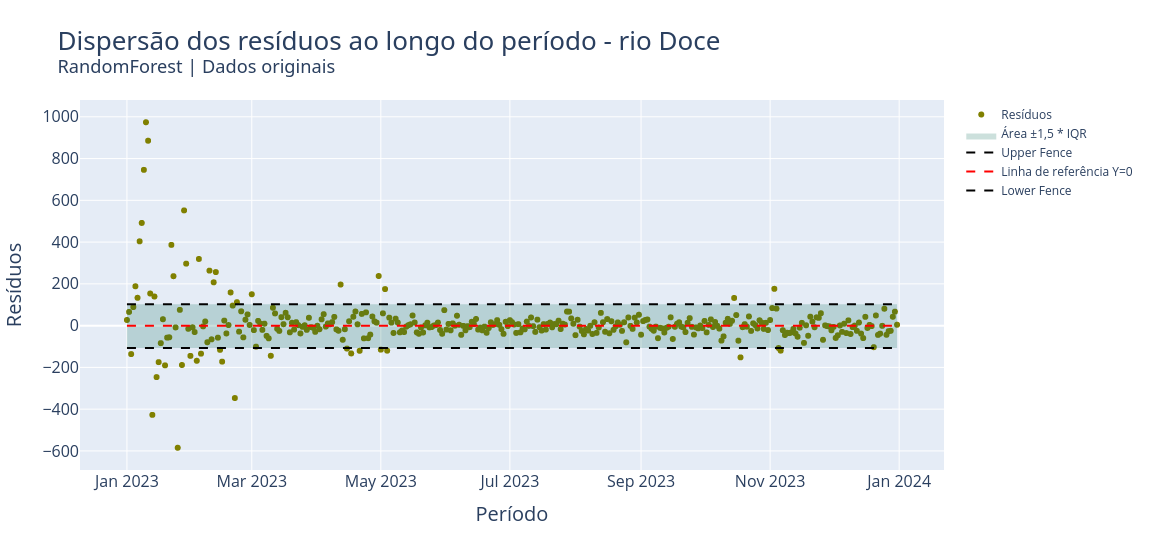
\includegraphics[scale=0.33]{Figuras/rio_doce/wfv/RF/RF_WFV_ORIG_RESID_x_TEMPO.png}
	\caption{Dispersão dos resíduos ao longo do ano.\\(fonte: o autor)}
	\label{fig:doce_RF_WFV_ORIG_RESID_x_TEMPO}
\end{figure}
\clearpage

A assimetria dos resíduos para o modelo CB - figura \ref{fig:doce_CB_WFV_ORIG_RESID_x_CURVA_NORMAL} - é de $4,16$, o que indica uma distribuição altamente assimétrica à direita e positiva. Isso quer dizer que os erros positivos são mais frequentes ou mais intensos do que os erros negativos, o que combina com o viés sistemático ds modelo em que o PBIAS indicou subestimação - visto em \ref{fig:doce_CB_WFV_ORIG}. Posto que o cálculo do resíduo é ``$observado - previsto$'' e trazendo o gráfico \ref{fig:doce_CB_WFV_ORIG_RESID_x_TEMPO} à vista aqui novamente, percebe-se que esta cauda longa de valores positivos ocorreu principalmente no início do ano, exatamente quando as variações nas vazões foram mais intensas. Este fenômeno também ocorreu com os outros modelos - figuras \ref{fig:doce_LR_WFV_LOG_RESID_x_CURVA_NORMAL} e \ref{fig:doce_RF_WFV_ORIG_RESID_x_CURVA_NORMAL}. Contudo, para o modelo LR com dados log-transformados, a assimetria se mostrou menor - $2,71$ - do que em relação aos modelos não-lineares, restando a assimetria de $3,24$ para o modelo RF. Nesta avaliação, o modelo CB apresentou a pior distribuição de resíduos, abrindo margem para melhorias. O mesmo, no entanto, vale para os modelos LR e RF que também apresentaram assimetria elevada e carecem de aprimoramentos.

A curva normal - em vermelho - está deslocada à direita, devido a assimetria dos dados, para todos os modelos, porém um pouco menos para o modelo LR. Todos os modelos possuem resíduos concentrados, majoritariamente, entre $-200$ e $200$, contudo, para os modelos não-lineares CB e RF, a variação total dos resíduos oscila entre aproximadamente $-550$ e $1000$, ao passo que o modelo LR, mostrando melhor comportamento, oscila entre $-400$ e aproximadamente $750$. Isso tudo mostra os modelos não capturaram bem as dinâmicas quando de valores mais elevados de vazão.

\begin{figure}[!h]
	\centering
	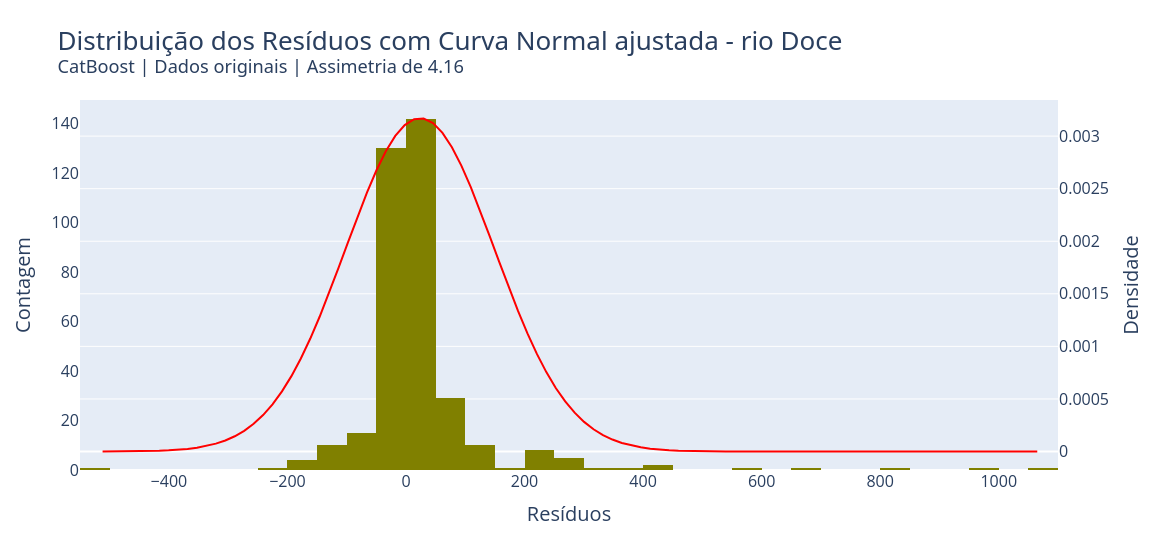
\includegraphics[scale=0.33]{Figuras/rio_doce/wfv/CB/CB_WFV_ORIG_RESID_x_CURVA_NORMAL.png}
	\caption{Histograma e curva-normal dos resíduos.\\(fonte: o autor)}
	\label{fig:doce_CB_WFV_ORIG_RESID_x_CURVA_NORMAL}
\end{figure}

\begin{figure}[!h]
	\centering
	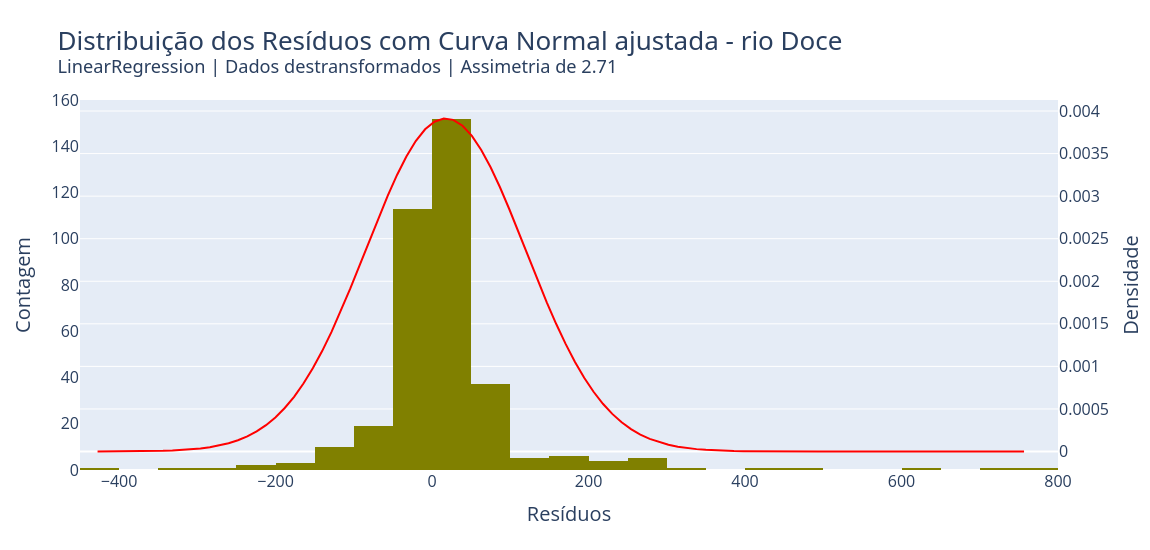
\includegraphics[scale=0.33]{Figuras/rio_doce/wfv/LR/LR_WFV_LOG_RESID_x_CURVA_NORMAL.png}
	\caption{Histograma e curva-normal dos resíduos.\\(fonte: o autor)}
	\label{fig:doce_LR_WFV_LOG_RESID_x_CURVA_NORMAL}
\end{figure}

\begin{figure}[!h]
	\centering
	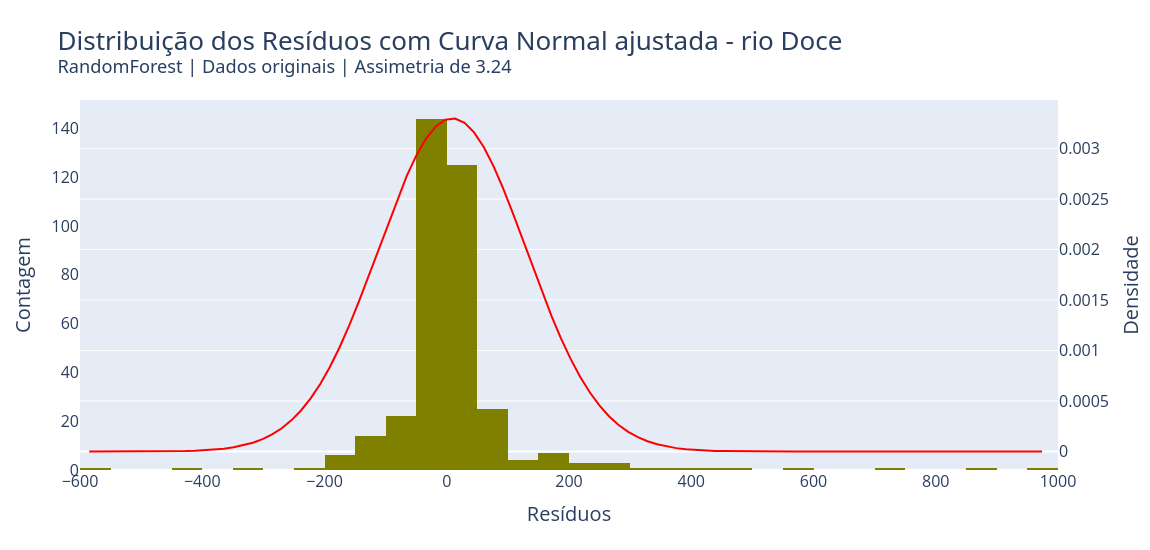
\includegraphics[scale=0.33]{Figuras/rio_doce/wfv/RF/RF_WFV_ORIG_RESID_x_CURVA_NORMAL.png}
	\caption{Histograma e curva-normal dos resíduos.\\(fonte: o autor)}
	\label{fig:doce_RF_WFV_ORIG_RESID_x_CURVA_NORMAL}
\end{figure}
\clearpage

O CB apresenta autocorrelação significativa nas primeiras \textit{lags} - até aproximadamente a \textit{lag} 10 -, com picos consideráveis de correlação positiva, indicando que o modelo está deixando dependências temporais nos resíduos - figura \ref{fig:doce_CB_WFV_ORIG_RESID_ACF}. Após as previsões imediatas, os resíduos ainda carregam dependências de eventos passados, o que não deveria ocorrer. O LR também mostra autocorrelação nas primeiras \textit{lags}, repetindo o comportamento do CB, embora de menor magnitude quando comparado a este - figura \ref{fig:doce_LR_WFV_LOG_RESID_ACF}. Ainda que o modelo LR também não esteja capturando completamente as dependências de curto prazo, ele o faz de forma um pouco mais eficiente que o CB. Por sua vez, o RF apresenta picos de autocorrelação menores que CB, igualmente baixo quanto o LR - até a \textit{lag} $2$ - nas primeiras \textit{lags} - figura \ref{fig:doce_RF_WFV_ORIG_RESID_ACF}. No entanto, ainda persiste alguma autocorrelação, com uma magnitude baixa, sugerindo que o RF está deixando passar para os resíduos uma dinâmica temporal.

Avançando no estudo, a autocorrelação do modelo CB diminui rapidamente após as primeiras \textit{lags} e por volta da \textit{lag} $10$, a maioria dos resíduos já se estabiliza dentro do intervalo de confiança - a área azul esmaecida. Isso é um sinal de que, a partir de \textit{lags} maiores, os resíduos são independentes, um comportamento esperado e positivo para previsões de longo prazo. Perceba, no entanto, que tanto o LR quanto o RF apresentam uma dissipação rápida da autocorrelação, diferentemente do CB, e seus resíduos se estabilizam rapidamente dentro do intervalo de confiança após as primeiras \textit{lags}.

Todos os modelos mostraram alguma autocorrelação nos resíduos de curto prazo, indicando que nenhum deles conseguiu eliminar completamente as dependências temporais de curto prazo. Esse fenômeno é mais acentuado no CB, seguido por LR e RF, que apresentaram a menor autocorrelação nas primeiras \textit{lags}. Essa presença presistente de autocorrelação nos resíduos significa que as previsões de curto prazo são influenciadas pelos eventos passados, sugerindo que os modelos não estão capturando eventos imediatamente próximos de maneira ideal.

\begin{figure}[!h]
	\centering
	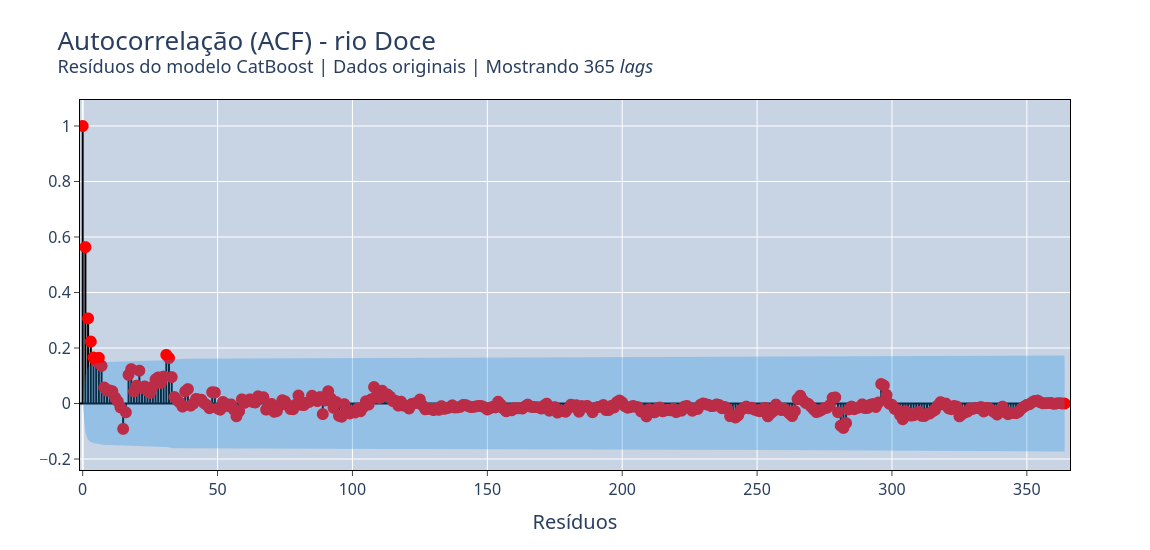
\includegraphics[scale=0.33]{Figuras/rio_doce/wfv/CB/CB_WFV_ORIG_RESID_ACF.png}
	\caption{Gráfico ACF dos resíduos.\\(fonte: o autor)}
	\label{fig:doce_CB_WFV_ORIG_RESID_ACF}
\end{figure}

\begin{figure}[!h]
	\centering
	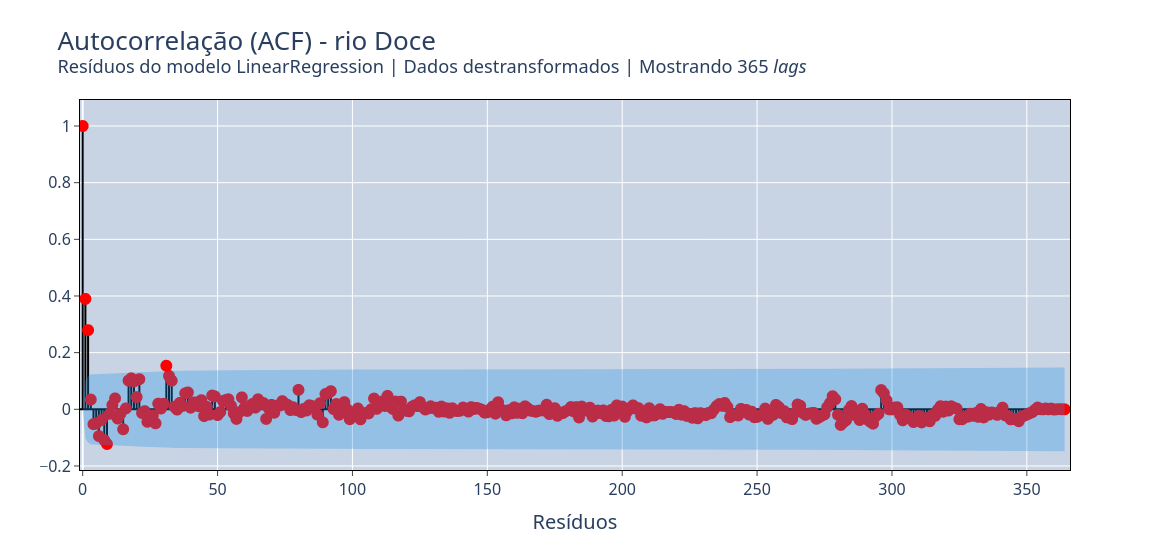
\includegraphics[scale=0.33]{Figuras/rio_doce/wfv/LR/LR_WFV_LOG_RESID_ACF.png}
	\caption{Gráfico ACF dos resíduos.\\(fonte: o autor)}
	\label{fig:doce_LR_WFV_LOG_RESID_ACF}
\end{figure}

\begin{figure}[!h]
	\centering
	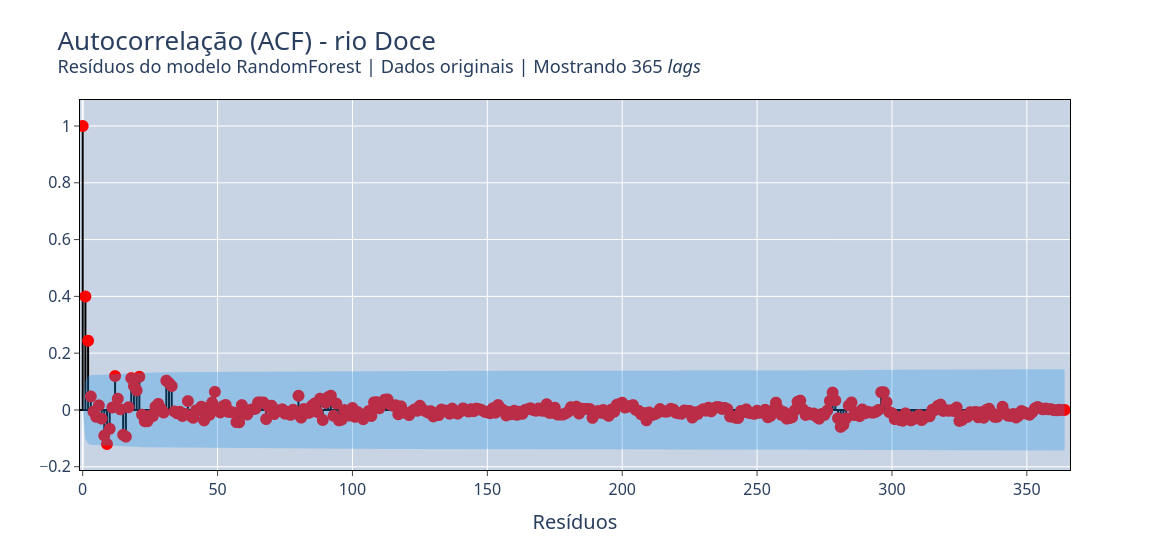
\includegraphics[scale=0.33]{Figuras/rio_doce/wfv/RF/RF_WFV_ORIG_RESID_ACF.png}
	\caption{Gráfico ACF dos resíduos.\\(fonte: o autor)}
	\label{fig:doce_RF_WFV_ORIG_RESID_ACF}
\end{figure}
\clearpage

Toda essa análise demonstrou aspectos importantes acerca dos modelos. Todos apresentaram uma tendência de subestimar os picos, com o modelo LR tendo uma oscilação levemente menor - de $-400$ a $750$ -, o período do ano que foi complicado para os modelos foi o período inicial do ano, verão, quando as vazões são fortemente impactadas pelas oscilações nas precipitações e o gráfico ACF deixou claro que os resíduos carregam dependência temporal de curto prazo. Isso sugere a necessidade de inclusão de mais variáveis explicativas para lidar com esses eventos extremos, refinamento nos hiperparâmetros - para os modelos não-lineares -, ou mesmo de refinamento nas técnicas de modelagem - isso não pode ser descartado.

\subsection{Rio Grande}

O rio Grande foi o único que a análise foi feita em uma massa reduzida de dados. Conforme já detalhado, apenas dados de setembro de $2020$ até dezembro de $2023$. Feita esta ressalva, os resultados mostraram-se bons e os modelos foram estáveis quando da análise dos resíduos. Perceba que aqui, para o modelo LR, os melhores resultados foram com os dados escalados MinMax e não os dados log-transformados.

Iniciando pela métrica KGE, aqui, o RF saiu-se melhor, seguido próximo pelo LR - figuras \ref{fig:grande_RF_WFV_ORIG} e \ref{fig:grande_LR_WFV_ORIG}, respectivamente. Ambos tiveram valores superiores ao CB - figura \ref{fig:grande_CB_WFV_ORIG} -, indicando que capturaram melhor correlação, viés e variabilidade nos dados previstos de vazão ao longo do período.

Sobre o erro médio (MAPE), o RF e o CB apresentaram os menores valores e próximos entre si, ou seja, ambos tiveram comportamento semelhante - valores de $0,123$ e $0,126$, respectivamente. O modelo LR ficou ligeiramente ruim, $0,133$, mas de toda forma, isso os coloca com resultados muito próximos, sugerindo que todos os três modelos ofereceram previsões de boa qualidade.

O LR tem a menor PBIAS - $-1,99\%$ -, suas previsões foram mais equilibradas, com menos tendência neste caso de subestimar os valores de vazão. O modelos CB e RF também têm PBIAS relativamente baixos - respectivamente $-4,44\%$ e $-2,18\%$ -, mas o CB apresentou um maior valor negativo pior, deixando clara uma subestimação elevada comparada aos outros modelos.

A cobertura empírica do LR é significativamente maior do que a dos outros dois modelos, com $84,38\%$, mostrando que o intervalo de previsão capturou com mais precisão a variabilidade real presente nas observações. Tanto o CB ($63,56\%$) quanto o RF ($63,01\%$) têm valores de cobertura mais baixos, que mostram, por sua vez, intervalos de previsão foram mais estreitos e não conseguiram captar toda a variabilidade observada nos dados reais.

Em ambos os modelos não-lineares a previsão segue de perto a série observada, mas a subestimação das vazões mais altas é evidente. O intervalo de previsão é estreito em momentos de pico, o que contribui para a baixa cobertura empírica calculada. Os maiores desvios nas previsões ocorrem em períodos de alta vazão (por volta de março e maio de $2023$), onde os modelos apresentaram dificuldade em acompanhar as flutuações nas vazões.

O modelo LR consegue capturar razoavelmente bem as flutuações de vazão, mas também apresenta comportamento tendencioso de subestimar os picos mais extremos, da mesma forma que os modelos CB e RF. Contudo, o intervalo de previsão foi o mais amplo dos três modelos, resultando em uma cobertura empírica maior.

O RF foi o modelo que obteve o melhor equilíbrio entre precisão (MAPE), correlação/variabilidade (KGE) e viés (PBIAS), mostrando um desempenho consistente. No entanto, a cobertura empírica baixa sugere que o intervalo de previsão não captura toda a incerteza associada aos dados, é uma característica que pode melhorar. O LR, embora tenha uma MAPE ligeiramente maior, apresentou o melhor valor de PBIAS, denotando que ele tem a menor tendência a viés sistemático entre os modelos. Além disso, sua maior cobertura empírica sugere que o modelo captura melhor a variabilidade dos dados. Finalmente, o CB, ainda que seja um modelo robusto, mostrou desempenho inferior em termos de KGE e PBIAS, mostrando dificuldades em capturar corretamente as variações sazonais e os picos extremos de vazão. Contudo, vale destacar, este é um modelo altamente personalizável e um procedimento de otimização dos hiperparâmetros pode verter melhores resultados.

\begin{figure}[!h]
	\centering
	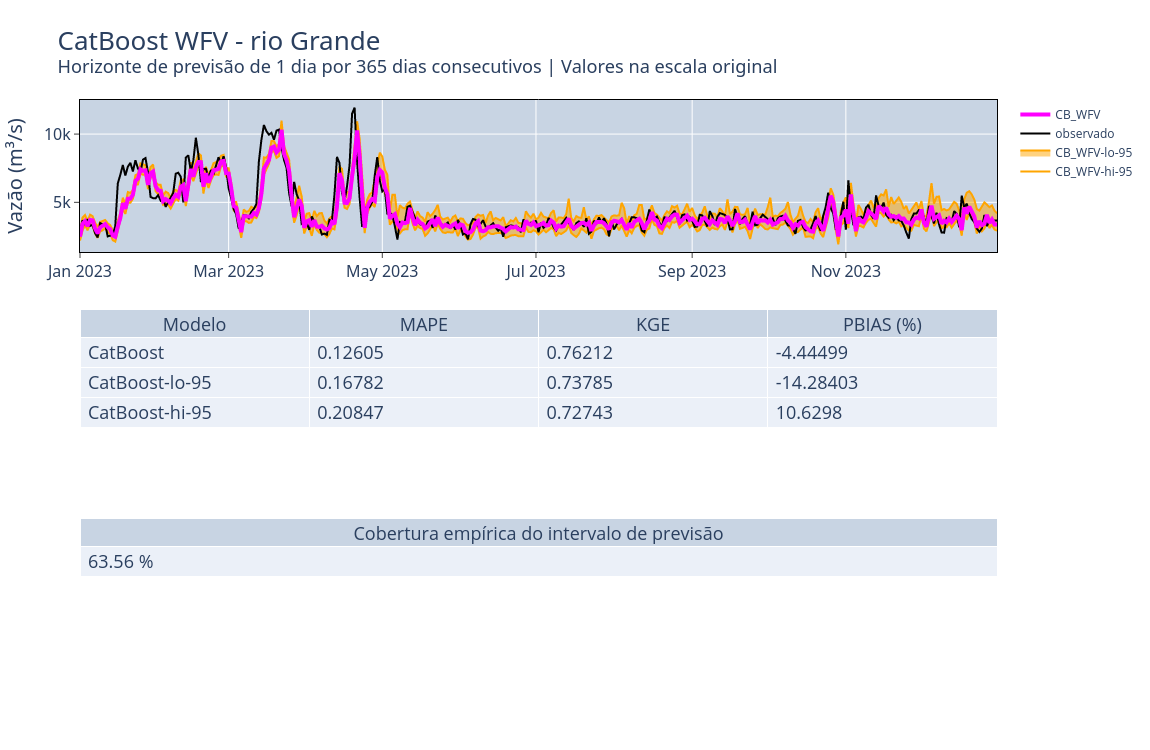
\includegraphics[scale=0.33]{Figuras/rio_grande/wfv/CB/CB_WFV_ORIG.png}
	\caption{\textit{Walk-Forward Validation} para o modelo CatBoost - CB.\\(fonte: o autor)}
	\label{fig:grande_CB_WFV_ORIG}
\end{figure}

\begin{figure}[!h]
	\centering
	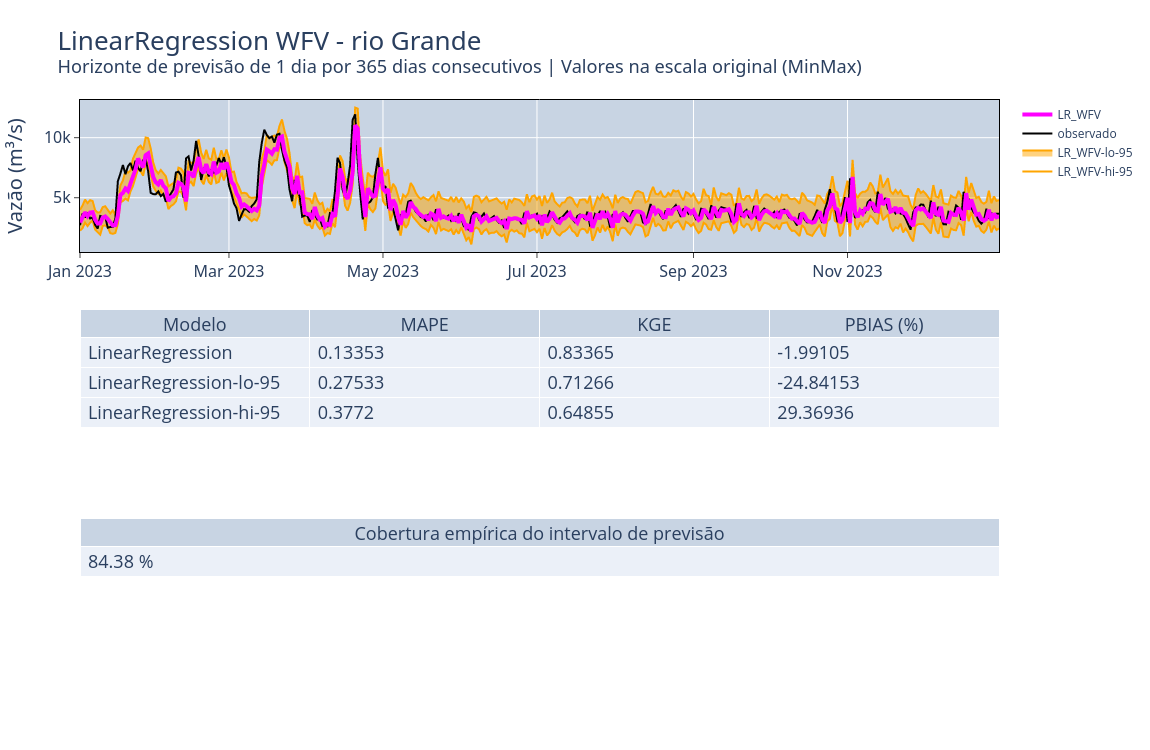
\includegraphics[scale=0.33]{Figuras/rio_grande/wfv/LR/LR_WFV_ORIG.png}
	\caption{\textit{Walk-Forward Validation} para o modelo LinearRegression - LR.\\(fonte: o autor)}
	\label{fig:grande_LR_WFV_ORIG}
\end{figure}

\begin{figure}[!h]
	\centering
	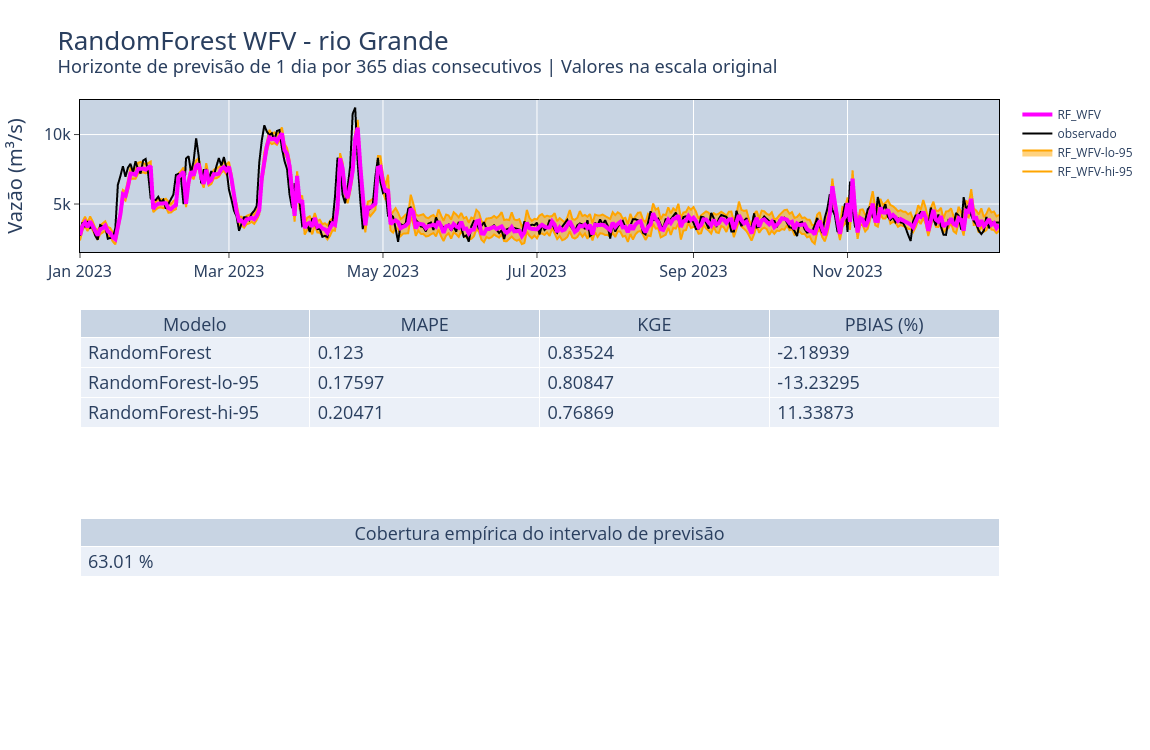
\includegraphics[scale=0.33]{Figuras/rio_grande/wfv/RF/RF_WFV_ORIG.png}
	\caption{\textit{Walk-Forward Validation} para o modelo RandomForest - RF.\\(fonte: o autor)}
	\label{fig:grande_RF_WFV_ORIG}
\end{figure}
\clearpage

%A análise dos gráficos de resíduos \textit{versus} valores previstos para os três modelos revela importantes diferenças no comportamento dos resíduos em relação às previsões. De início é possível notar as largas faixas de valores em que os resíduos se concentraram. O CB teve valores de \textit{lower fence} e \textit{upper fence} de $-1328,72$ e $1492,10$, respectivamente, uma amplitude de $2820$, o que lhe conferiu uma prevalência de $89,32\%$ dos resíduos dentro destes limites. De antemão, o menor valor dentre os modelos. Continuando para o modelo LR, tendo $-1628,38$ para o valor da faixa mínima e $1687,81$ para a máxima - amplitude de $3315$ - teve prevalência de 92,60\% dos resíduos. Isso parece realmente bom, mas com uma ampla faixa assim deixa indicado que o modelo oscilou muito nas previsões realizadas, demostrando incerteza. Finalmente, o RF, ficou ``no meio do caminho'' entre os modelos anteriores. Tendo os valores de $-1422,62$ para \textit{lower fence} e $1531,92$ para \textit{upper fence}, perfazendo uma amplitude de $2953$, o modelo teve prevalência de $90,68\%$ dos resíduos dentro destes limites.
%
%Olhando mais atentamente o gráfico do modelo CB - figura \ref{fig:grande_CB_WFV_ORIG_RESID_x_PREV} -, os resíduos estão relativamente concentrados em torno de $0$ para a maioria dos valores previstos. Contudo, à medida que os valores previstos aumentam, os resíduos se tornam mais dispersos, especialmente para previsões acima de $6000 m^3/s$. 
%
%O CB tende a subestimar mais frequentemente as previsões - maior presença de resíduos acima de \textit{upper fence} - para valores elevados de vazão. Existem vários \textit{outliers} positivos e negativos, com valores de resíduos superiores a $2000 m^3/s$ e inferiores a $-1.000 m^3/s$, principalmente para as previsões mais altas, donde pode-se inferir que o CB lidou bem com vazões mais baixas e moderadas, mas apresentou maior dificuldade com picos extremos de vazão, como indicado pela dispersão e pelos \textit{outliers} em previsões de alta magnitude.
%
%O modelo LR também apresentou distribuição de resíduos concentrada em torno de $0$ para valores previstos mais baixos - figura \ref{fig:grande_LR_WFV_ORIG_RESID_x_PREV}. No entanto, a \underline{dispersão} dos resíduos é maior em torno de $0$ e dentro do intervalo mostrado no gráfico, e houve alguns \textit{outliers} para previsões extremamente altas (acima de $7000 m^3/s$). Essa maior dispersão e alguns destes \textit{outliers} extremos indicam dificuldades do modelo em lidar com previsões de vazões de moderadas a extremas.
%
%O RF apresenta uma distribuição de resíduos relativamente mais compacta em torno de $0$ para a maioria dos valores previstos. No entanto, também há uma dispersão crescente à medida que os valores previstos aumentam, semelhante ao CB e ao LR. Um fato importante a se observar, colocando de lado os gráficos \ref{fig:grande_RF_WFV_ORIG_RESID_x_PREV} e \ref{fig:grande_CB_WFV_ORIG_RESID_x_PREV}, em que ambos os comportamentos se assemelham, apesar da faixa levemente larga e da menor prevalência dos resíduos dentro desta, o modelo CB apresentou menos resíduos de valores elevados \underline{abaixo} de \textit{lower fence}, ou seja, o modelo superestimou muito menos as previsões. Porém, acima de \textit{upper fence}, o CB teve mais pontos fora, reforçando o que já tinha sido apresentado antes através da PBIAS, de que este modelo teve tendência sistemática para subestimar as previsões. O modelo RF apresentou uma distribuição acima de \textit{upper fence} e abaixo de \textit{lower fence} mais equilibrada, uma amplitude mediana - quando vista ao lado dos outros modelos -, elevada concentração dos resíduos próximo a $0$, o que faz indicar um comportamento estável holisticamente. Também teve problemas em captar vazões extremas, de certo, mas quando se considera outros parâmetros para mensurar a qualidade, este modelo ficou em um ponto central. E, assim como o CB, ainda pode ser melhorado por otimização de hiperparâmetros.
%
%Quando fala-se em precisão, todos os três modelos - CB, LR e RF - apresentaram resíduos concentrados em torno de $0$ para valores previstos moderados (entre $3000$ e $6000 m^3/s$), indicando que eles conseguem lidar bem com a previsão de vazões nessa faixa, mas para valores extremos, ainda que eventualmente um modelo tenha sido melhor que o outro, foi muito pequena a variação, deixando claro que as previsões extremas foram problemáticas para todos os modelos.
%
%\begin{figure}[!h]
%	\centering
%	\includegraphics[scale=0.33]{Figuras/rio_grande/wfv/CB/CB_WFV_ORIG_RESID_x_PREV.png}
%	\caption{Dispersão dos resíduos.\\(fonte: o autor)}
%	\label{fig:grande_CB_WFV_ORIG_RESID_x_PREV}
%\end{figure}
%
%\begin{figure}[!h]
%	\centering
%	\includegraphics[scale=0.33]{Figuras/rio_grande/wfv/LR/LR_WFV_ORIG_RESID_x_PREV.png}
%	\caption{Dispersão dos resíduos.\\(fonte: o autor)}
%	\label{fig:grande_LR_WFV_ORIG_RESID_x_PREV}
%\end{figure}
%
%\begin{figure}[!h]
%	\centering
%	\includegraphics[scale=0.33]{Figuras/rio_grande/wfv/RF/RF_WFV_ORIG_RESID_x_PREV.png}
%	\caption{Dispersão dos resíduos.\\(fonte: o autor)}
%	\label{fig:grande_RF_WFV_ORIG_RESID_x_PREV}
%\end{figure}
%\clearpage

A análise dos gráficos de dispersão dos resíduos ao longo do tempo para os modelos revela informações importantes sobre a evolução do desempenho de cada modelo em termos de erro durante o período analisado para o rio Grande. Aqui é possível identificar padrões de erro, presença de \textit{outliers} e a estabilidade dos resíduos ao longo do tempo.

De início é possível notar as largas faixas de valores em que os resíduos se concentraram. O CB teve valores de \textit{lower fence} e \textit{upper fence} de $-1328,72$ e $1492,10$, respectivamente, uma amplitude de $2820$, o que lhe conferiu uma prevalência de $89,32\%$ dos resíduos dentro destes limites. De antemão, o menor valor dentre os modelos. Continuando para o modelo LR, tendo $-1628,38$ para o valor da faixa mínima e $1687,81$ para a máxima - amplitude de $3315$ - teve prevalência de $92,60\%$ dos resíduos. Isso parece realmente bom, mas com uma ampla faixa assim deixa indicado que o modelo oscilou muito nas previsões realizadas, demostrando incerteza. Finalmente, o RF, ficou ``no meio do caminho'' entre os modelos anteriores, tendo valores de $-1422,62$ para \textit{lower fence} e $1531,92$ para \textit{upper fence}, perfazendo uma amplitude de $2953$, o modelo teve prevalência de $90,68\%$ dos resíduos dentro da área sombreada.

O modelo CB demonstra uma concentração dos resíduos dentro da faixa de $\pm 1000 m^3/s$ na maior parte do período estudado - figura \ref{fig:grande_CB_WFV_ORIG_RESID_x_TEMPO}. Contudo, nos primeiros meses, de janeiro a maio de $2023$, observa-se um maior espalhamento dos resíduos, com vários pontos excedendo os $2000 m^3/s$. A presença de \textit{outliers} entre março e maio de $2023$ indica que o modelo enfrentou dificuldades para lidar com picos de vazão nesse período, ocasionando erros elevados. Apesar disso, após o pico de erro em maio, os resíduos tornaram-se mais constantes, com variações menores e mais previsíveis, embora alguns \textit{outliers} persistam no final do ano, demonstrando, desta forma, que há desafios na captura de variações extremas.

Em contraste, o LR apresenta uma dispersão dos resíduos significativamente maior ao longo do tempo quando comparada ao CB - figura \ref{fig:grande_LR_WFV_ORIG_RESID_x_TEMPO} e é possível inferir isso olhando para a larga amplitude dos limites da área sombreada - $\pm 1,5 \times IQR$. Mesmo nos períodos de menor erro, como de julho a novembro de $2023$, os resíduos ainda apresentam uma variação considerável, ainda muito dispersos, distantes da reta de referência $y=0$. A estabilidade dos resíduos da LR ficou, assim, comprometida e é verificável pela elevada dispersão mesmo em períodos em que a série de dados observados apresentou vazões estáveis e mais moderadas. Essa variabilidade reflete a limitação do LR em capturar a complexidade dos dados de vazão, com dados de treinamento muito ruidosos - figura \ref{fig:serie_completa_estacao_t_vz_62020080}, revelando que o LR não lidou adequadamente com eventos extremos de vazão.

Por sua vez, o RF apresenta uma dispersão dos resíduos semelhante à do CB - figura \ref{fig:grande_RF_WFV_ORIG_RESID_x_TEMPO} -, porém com uma leve quantidade menor de \textit{outliers} - $35$ pontos fora da área demarcada contra $39$ pontos fora para o modelo CB -, considerando acima de \textit{upper fence} e abaixo de \textit{lower fence}. A maior parte dos resíduos do RF está confinada à faixa de $\pm 1000 m^3/s$, com algumas exceções nos meses de março e abril e também os meses de novembro e dezembro de $2023$, onde o modelo aparentou maior dificuldade em prever corretamente as vazões. A presença reduzida de \textit{outliers} no RF, em comparação ao CB, bem como uma amplitude menor comparada ao LR, sugere uma maior robustez na captura das variações de vazão ao longo do tempo, embora alguns \textit{outliers} ocorram durante períodos de maior instabilidade nas vazões.

De maneira geral, tanto o CB quanto o RF demonstraram um padrão de erro mais estável ao longo do tempo, com a maioria dos resíduos concentrados dentro de uma faixa controlada de $\pm 1000 m^3/s$. Ambos os modelos apresentaram períodos de erro maior, especialmente no início do ano, mas tendem a estabilizar conforme o tempo avança. Em contrapartida, o LR exibiu elevada variabilidade nos resíduos, indicando uma menor capacidade de lidar com as flutuações nas vazões independentemente do período analisado.

\begin{figure}[!h]
	\centering
	\includegraphics[scale=0.33]{Figuras/rio_grande/wfv/CB/CB_WFV_ORIG_RESID_x_TEMPO.png}
	\caption{Dispersão dos resíduos ao longo do ano.\\(fonte: o autor)}
	\label{fig:grande_CB_WFV_ORIG_RESID_x_TEMPO}
\end{figure}

\begin{figure}[!h]
	\centering
	\includegraphics[scale=0.33]{Figuras/rio_grande/wfv/LR/LR_WFV_ORIG_RESID_x_TEMPO.png}
	\caption{Dispersão dos resíduos ao longo do ano.\\(fonte: o autor)}
	\label{fig:grande_LR_WFV_ORIG_RESID_x_TEMPO}
\end{figure}

\begin{figure}[!h]
	\centering
	\includegraphics[scale=0.33]{Figuras/rio_grande/wfv/RF/RF_WFV_ORIG_RESID_x_TEMPO.png}
	\caption{Dispersão dos resíduos ao longo do ano.\\(fonte: o autor)}
	\label{fig:grande_RF_WFV_ORIG_RESID_x_TEMPO}
\end{figure}
\clearpage

O CB apresentou assimetria de $1,3$, o que significa uma distribuição levemente assimétrica para a direita. Embora a maior parte dos resíduos estivesse concentrada próximo a $0$, houve uma quantidade considerável de erros positivos, especialmente para valores acima de $2000$. A curva normal ajuda a demonstrar que os resíduos seguem uma forma próxima da normalidade, porém com uma cauda longa à direita. Esse comportamento significa que o CB tende a cometer alguns erros maiores nas previsões de altas vazões, subestimando estas vazões mais extremas - figura \ref{fig:grande_CB_WFV_ORIG_RESID_x_CURVA_NORMAL}.

Em contraste, o LR apresentou uma assimetria de $0,97$, ou seja, a distribuição dos resíduos no modelo LR foi quase simétrica, com um leve desvio à direita. Os erros estiveram razoavelmente bem concentrados em torno de $0$, apesar da grande variabilidade mencionada anteriormente, com uma leve tendência de subestimativas. Contudo, ainda houve resíduos significativos acima de $1500 m^3/s$, mostrando que o LR não capturou adequadamente as variações maiores nas vazões - figura \ref{fig:grande_LR_WFV_ORIG_RESID_x_CURVA_NORMAL}.

O RF apresentou a menor assimetria entre os três modelos, com um valor de $0,82$, a distribuição de resíduos mais simétrica entre todos. O RF lidou melhor com os erros, distribuindo-os de maneira mais uniforme em torno de $0$, concentrando os resíduos, em sua maior parte, na faixa $\pm 1000 m^3/s$, e teve a distribuição dos resíduos mais precisa, seguindo a forma da curva normal em comparação com o CB e o LR. Isso indica que o modelo RF teve uma maior capacidade de gerar previsões com erros menores e menos dispersos, o que ajuda a reforçar o resultado visto pelas métricas KGE ($0,83$) e MAPE ($0,12$). Este comportamento e todo este entendimento sugerem ao modelo RF uma maior robustez na gestão de valores extremos de vazão - figura \ref{fig:grande_RF_WFV_ORIG_RESID_x_CURVA_NORMAL}.

\begin{figure}[!h]
	\centering
	\includegraphics[scale=0.33]{Figuras/rio_grande/wfv/CB/CB_WFV_ORIG_RESID_x_CURVA_NORMAL.png}
	\caption{Histograma e curva-normal dos resíduos.\\(fonte: o autor)}
	\label{fig:grande_CB_WFV_ORIG_RESID_x_CURVA_NORMAL}
\end{figure}

\begin{figure}[!h]
	\centering
	\includegraphics[scale=0.33]{Figuras/rio_grande/wfv/LR/LR_WFV_ORIG_RESID_x_CURVA_NORMAL.png}
	\caption{Histograma e curva-normal dos resíduos.\\(fonte: o autor)}
	\label{fig:grande_LR_WFV_ORIG_RESID_x_CURVA_NORMAL}
\end{figure}

\begin{figure}[!h]
	\centering
	\includegraphics[scale=0.33]{Figuras/rio_grande/wfv/RF/RF_WFV_ORIG_RESID_x_CURVA_NORMAL.png}
	\caption{Histograma e curva-normal dos resíduos.\\(fonte: o autor)}
	\label{fig:grande_RF_WFV_ORIG_RESID_x_CURVA_NORMAL}
\end{figure}
\clearpage

Os gráficos ACF de todos os modelos demonstraram que as primeiras $30$ \textit{lags} apresentaram autocorrelação significativa e positiva. Este comportamento mostra a presença de uma estrutura nos resíduos que não foi completamente capturada pelos modelos, sugerindo que ainda mantiveram dependências temporais não modeladas de forma adequada. A partir da \textit{lag} $30$, aproximadamente \textit{lag} $45$ para o LR, as correlações caíram dentro da faixa de confiança - área azul clara -, sinalizando uma melhora na independência dos resíduos. No entanto, as flutuações entre autocorrelações positivas e negativas dentro dessa faixa ainda foram perceptíveis.

Com o modelo RF foi menos, mas para os modelos CB e LR é possível reparar inclusive um comportamento sazonal nas \textit{lags} iniciais do gráfico, deixando ainda mais evidente que houve comportamento temporal que os modelos não capturaram adequadamente.

As conclusões gerais indicam que todos os modelos apresentaram algum nível de autocorrelação significativa nas primeiros \textit{lags}, nenhum deles conseguiu modelar completamente as dependências temporais presentes nos dados. Isso aponta para a possibilidade de melhorias, como, por exemplo, a incorporação de mecanismos para lidar com sazonalidade ou dependência temporal de forma mais direta, por exemplo, \textit{features} de \textit{lag} mais robustas. Cabe destacar ainda que a qualidade dos dados de treinamento também exerce influência neste resultado por parte dos modelos, basta comparar com os outros rios.

Resultados visíveis nas figuras \ref{fig:grande_CB_WFV_ORIG_RESID_ACF}, \ref{fig:grande_LR_WFV_ORIG_RESID_ACF} e \ref{fig:grande_RF_WFV_ORIG_RESID_ACF}.

\begin{figure}[!h]
	\centering
	\includegraphics[scale=0.33]{Figuras/rio_grande/wfv/CB/CB_WFV_ORIG_RESID_ACF.png}
	\caption{Gráfico ACF dos resíduos.\\(fonte: o autor)}
	\label{fig:grande_CB_WFV_ORIG_RESID_ACF}
\end{figure}

\begin{figure}[!h]
	\centering
	\includegraphics[scale=0.33]{Figuras/rio_grande/wfv/LR/LR_WFV_ORIG_RESID_ACF.png}
	\caption{Gráfico ACF dos resíduos.\\(fonte: o autor)}
	\label{fig:grande_LR_WFV_ORIG_RESID_ACF}
\end{figure}

\begin{figure}[!h]
	\centering
	\includegraphics[scale=0.33]{Figuras/rio_grande/wfv/RF/RF_WFV_ORIG_RESID_ACF.png}
	\caption{Gráfico ACF dos resíduos.\\(fonte: o autor)}
	\label{fig:grande_RF_WFV_ORIG_RESID_ACF}
\end{figure}
\clearpage

\subsection{Rio São Francisco}

A análise comparativa dos desempenhos dos três modelos de previsão revelou variações significativas em termos de robustez, precisão e capacidade de capturar a variabilidade dos dados de vazão ao longo de um ano.

O CB apresentou uma KGE de $0,93$ - figura \ref{fig:francisco_CB_WFV_ORIG} -, indicando uma boa eficiência nas previsões e demonstrando que o modelo conseguiu replicar o comportamento hidrológico observado de forma consistente. O LR destacou-se com o maior valor de KGE, atingindo $0,98$ - figura \ref{fig:francisco_LR_WFV_LOG} -, o que corroborou sua elevada capacidade preditiva e eficiência em relação aos dados observados. O RF apresentou um KGE de $0,97$, o que demonstra uma ótima qualidade de previsão, que se aproximou consideravelmente dos valores observados, embora ligeiramente inferior ao do modelo LR - figura \ref{fig:francisco_RF_WFV_ORIG}.

Em seguida, a métrica de MAPE foi analisada. O CB exibiu um MAPE de $0,032$, o que é um erro percentual médio absoluto muito baixo. O LR apresentou uma MAPE de $0,027$ e o RF $0,025$, os dois modelos com o melhor resultado, sendo o RF levemente melhor. Mas em termos práticos, ambos os modelos tiveram a mesma qualidade no erro médio das previsões. Considerando o resultado da KGE, até este momento, os dois modelos ficaram quase idênticos.

Quanto à PBIAS, o CB apresentou um valor de $-2,61\%$, evidenciando um leve viés negativo, o que indica que o modelo tende a subestimar as vazões previstas. O LR registrou um PBIAS mediano entre os modelos, com $-0,98\%$, indicando ainda um viés sistemático de subestimar as previsões, mas tão baixo que é quase desconsiderável. Um desempenho excelente. Mas agora, o RF exibiu um PBIAS de $-0,80\%$, o menor viés dentre todos os modelos, ainda com subestimação, porém, assim como o LR, baixíssimo, as previsões praticamente ``acertaram'' os valores observados. Em suma, neste ponto, todos os modelos apresentaram viés sistemático de subestimação, com o CB ficando com o resultado que pode ser chamado de ``pior''.

Por fim, quanto à cobertura empírica. O CB cobriu $90,68\%$ dos dados, demonstrando uma boa capacidade de captura das incertezas nas previsões. O LR alcançou a maior cobertura empírica, com $96,71\%$, tendo o intervalo de previsão com o melhor desempenho, o modelo capturou quase todos os eventos da série de vazões observadas. O RF, por sua vez, apresentou a menor cobertura empírica, com $82,47\%$, o que indica que o intervalo de previsão gerado pelo RF foi mais estreito e possivelmente não capturou todas as variações na série de vazão.

O LR destacou-se como o modelo com maior eficiência na replicação do comportamento hidrológico observado, evidenciado pelo maior valor de KGE, a MAPE e PBIAS medianas entre os modelos e pela cobertura empírica mais alta. Porém, de forma geral, todos os modelos apresentaram resultados competitivos e para os dados do rio São Francisco se mostraram altamente eficientes.

\begin{figure}[!h]
	\centering
	\includegraphics[scale=0.33]{Figuras/rio_sao_francisco/wfv/CB/CB_WFV_ORIG.png}
	\caption{\textit{Walk-Forward Validation} para o modelo CatBoost - CB.\\(fonte: o autor)}
	\label{fig:francisco_CB_WFV_ORIG}
\end{figure}

\begin{figure}[!h]
	\centering
	\includegraphics[scale=0.33]{Figuras/rio_sao_francisco/wfv/LR/LR_WFV_LOG.png}
	\caption{\textit{Walk-Forward Validation} para o modelo LinearRegression - LR.\\(fonte: o autor)}
	\label{fig:francisco_LR_WFV_LOG}
\end{figure}

\begin{figure}[!h]
	\centering
	\includegraphics[scale=0.33]{Figuras/rio_sao_francisco/wfv/RF/RF_WFV_ORIG.png}
	\caption{\textit{Walk-Forward Validation} para o modelo RandomForest - RF.\\(fonte: o autor)}
	\label{fig:francisco_RF_WFV_ORIG}
\end{figure}
\clearpage

%No modelo CB, a maioria dos resíduos concentrou-se dentro da faixa delimitada por $\pm 1,5\times IQR$, com pontos ultrapassando mais o limite superior (\textit{upper fence}) do que o inferior (\textit{lower fence}). Isso remete à subestimação nas previsões, como apontando na métrica PBIAS, vista anteriormente. Nota-se uma tendência de aumento da variabilidade dos resíduos conforme os valores previstos aumentavam, sugerindo que o modelo enfrenta maior dificuldade em capturar corretamente vazões extremas. No entanto, de maneira geral, os resíduos ficaram bem distribuídos em torno da linha de referência, o que pode ser encarado como um bom ajuste global. Mesmo que tenha havido \textit{outliers}, o modelo mostrou-se estável, especialmente para vazões moderadas - figura \ref{fig:francisco_CB_WFV_ORIG_RESID_x_PREV}.
%
%O LR apresentou uma leve concentração em torno de $0$ para a grande parte dos valores previstos.
%
%Contudo, identificou-se uma maior quantidade de resíduos dispersos, indicando uma variação mais ampla dos erros. Essa dispersão sugeriu que o modelo linear possuía limitações em capturar a complexidade dos dados, especialmente para valores de vazão mais elevados, onde o modelo tendia a subestimar ou superestimar os valores observados com maior frequência. Embora a LR apresentasse uma cobertura mais ampla dos intervalos de previsão, a quantidade de resíduos fora do intervalo interquartílico (IQR) foi superior à do CatBoost, indicando uma menor robustez.
%
%O modelo RandomForest, por sua vez, demonstrou uma distribuição de resíduos bastante controlada, semelhante à do CatBoost, com a maioria dos resíduos concentrados dentro da faixa de ±100 m³/s em torno da linha de referência zero. O RF destacou-se por apresentar menos outliers, evidenciando uma maior estabilidade, principalmente para previsões de menor magnitude. No entanto, assim como nos outros modelos, foi possível notar uma dispersão um pouco maior à medida que os valores previstos aumentavam, o que indicou que o modelo enfrentava desafios em prever picos de vazão com precisão absoluta.
%
%Em termos comparativos, o modelo CatBoost apresentou um bom equilíbrio entre variabilidade e precisão, com resíduos bem distribuídos, mas com alguns outliers presentes, especialmente para valores previstos maiores. A Regressão Linear, embora mostrasse uma boa cobertura de intervalo, exibiu maior dispersão nos resíduos e uma quantidade mais expressiva de outliers, refletindo suas limitações em prever vazões em cenários mais extremos. Já o RandomForest mostrou-se o mais estável dos três modelos, com uma boa concentração de resíduos próximos a zero e menos outliers, sugerindo que ele lidava melhor com a variabilidade das vazões ao longo do tempo.
%
%Concluiu-se que o RandomForest parecia ser o modelo mais robusto e estável, especialmente no que diz respeito à captura de picos de vazão com menos outliers. O CatBoost também demonstrou um bom desempenho, mas com uma leve tendência a apresentar maior variabilidade para picos de vazão, o que poderia requerer ajustes adicionais. A Regressão Linear, por outro lado, apresentou limitações significativas em relação à complexidade dos dados, com uma maior dispersão dos resíduos e mais outliers, tornando-se o modelo menos indicado para prever vazões de maneira precisa e consistente.
%
%\begin{figure}[!h]
%\centering
%\includegraphics[scale=0.33]{Figuras/rio_sao_francisco/wfv/CB/CB_WFV_ORIG_RESID_x_PREV.png}
%\caption{Dispersão dos resíduos.\\(fonte: o autor)}
%\label{fig:francisco_CB_WFV_ORIG_RESID_x_PREV}
%\end{figure}
%
%\begin{figure}[!h]
%\centering
%\includegraphics[scale=0.33]{Figuras/rio_sao_francisco/wfv/LR/LR_WFV_LOG_RESID_x_PREV.png}
%\caption{Dispersão dos resíduos.\\(fonte: o autor)}
%\label{fig:francisco_LR_WFV_ORIG_RESID_x_PREV}
%\end{figure}
%
%\begin{figure}[!h]
%\centering
%\includegraphics[scale=0.33]{Figuras/rio_sao_francisco/wfv/RF/RF_WFV_ORIG_RESID_x_PREV.png}
%\caption{Dispersão dos resíduos.\\(fonte: o autor)}
%\label{fig:francisco_RF_WFV_ORIG_RESID_x_PREV}
%\end{figure}
%\clearpage

A análise comparativa dos resíduos dos modelos para o rio São Francisco revelou informações detalhadas sobre a precisão e robustez de cada abordagem ao longo do período de estudo.

Inicialmente, observou-se que a área sombreada nos gráficos de dispersão dos resíduos permaneceu bastante estreita para todos os modelos. Este comportamento indica que os modelos apresentaram uma alta precisão nos valores previstos, refletindo uma capacidade robusta de captura das tendências gerais das vazões.

Especificamente, o modelo CB apresentou um limie \textit{upper fence} de $103,87$ e \textit{lower fence} de $-72,34$, resultando em uma amplitude de $176,21$, com prevalência dos resíduos dentro desses limites de $83,84\%$. Contudo, o CB exibiu resíduos discrepantes no início do ano, especialmente em janeiro e fevereiro, antes de estabilizar a partir de março, restringindo-se à área de tolerância - figura \ref{fig:francisco_CB_WFV_ORIG_RESID_x_TEMPO}. Na porção final do ano, o modelo voltou a apresentar alguns valores discrepantes, embora a vasta maioria dos resíduos permanecesse próxima do limite superior.

Por sua vez, o modelo LR apresentou um \textit{upper fence} de $67,78$ e um \textit{lower fence} de $-48,93$, com uma amplitude de $116,71$ e uma prevalêcia de $81,92\%$. Embora o LR também tenha exibido resíduos discrepantes no início do ano, a quantidade foi menor comparada ao CB e ao RF, e a estabilização dos resíduos ocorreu apenas a partir de março. Na porção final do período, o LR mostrou um aumento no número de resíduos fora das faixas estabelecidas, tanto acima quanto abaixo dos limites, indicando uma menor robustez em comparação ao CB para este período. A amplitude dos resíduos da LR variou entre $-600$ e $600$, sendo menor quando comparada aos outros modelos. Adicionalmente, o LR apresentou um maior número de \textit{outliers} acima do limite superior, similar ao RF, e menos \textit{outliers} abaixo do limite inferior - figura \ref{fig:francisco_LR_WFV_LOG_RESID_x_TEMPO}.

O RF exibiu um limite superior de $46,83$ e inferior de $-39,87$, resultando em uma amplitude de $86,70$ e prevalência de $74,52\%$ dos resíduos na área sombreada, demonstrando uma distribuição de resíduos bastante controlada em torno da linha de referência $0$. No entanto, o RF também apresentou diversos \textit{outliers} no início do ano, de janeiro a março, e demorou para estabilizar na porção central do período, semelhante ao comportamento do LR. Na porção final do período, o RF voltou a apresentar muitos \textit{outliers}, e um maior espalhamento, refletindo desafios na previsão de vazões extremas. A amplitude dos resíduos do RF variou entre $-600$ e $600$, igualando-se à da LR - figura \ref{fig:francisco_RF_WFV_ORIG_RESID_x_TEMPO}.

De maneira geral, os modelos demonstraram que, durante períodos de variações elevadas nas precipitações e, consequentemente, nas vazões, apresentaram resultados incertos, evidenciados pela quantidade de \textit{outliers} tanto no início quanto no final do ano, com um resultado levemente melhor para o CB que teve menos \textit{outliers}. Ao que tudo indica, houve um certo atraso dos modelos em capturar eventos extremos, levando-os a dificuldades em responder rapidamente às mudanças abruptas nas condições hidrológicas. O CB apresentou uma boa prevalência dos resíduos na área entre $\pm 1,5 \times IQR$, apesar de algumas discrepâncias em períodos de alta variabilidade. O LR, embora com uma prevalência menor, apresentou também menor amplitude, houve equilíbrio entre estes dois aspectos, embora também tenha tido problemas com vazões extremas. O RF, apesar de sua estabilidade geral, também enfrentou desafios semelhantes em períodos de alta variabilidade. Estes resultados destacam a necessidade de aprimoramentos nos modelos para melhor capturar e responder a eventos hidrológicos extremos, potencialmente através da incorporação de mecanismos adicionais para lidar com sazonalidade e dependências temporais.

\begin{figure}[!h]
\centering
\includegraphics[scale=0.33]{Figuras/rio_sao_francisco/wfv/CB/CB_WFV_ORIG_RESID_x_TEMPO.png}
\caption{Dispersão dos resíduos ao longo do ano.\\(fonte: o autor)}
\label{fig:francisco_CB_WFV_ORIG_RESID_x_TEMPO}
\end{figure}

\begin{figure}[!h]
\centering
\includegraphics[scale=0.33]{Figuras/rio_sao_francisco/wfv/LR/LR_WFV_LOG_RESID_x_TEMPO.png}
\caption{Dispersão dos resíduos ao longo do ano.\\(fonte: o autor)}
\label{fig:francisco_LR_WFV_LOG_RESID_x_TEMPO}
\end{figure}

\begin{figure}[!h]
\centering
\includegraphics[scale=0.33]{Figuras/rio_sao_francisco/wfv/RF/RF_WFV_ORIG_RESID_x_TEMPO.png}
\caption{Dispersão dos resíduos ao longo do ano.\\(fonte: o autor)}
\label{fig:francisco_RF_WFV_ORIG_RESID_x_TEMPO}
\end{figure}
\clearpage

A análise comparativa dos resíduos dos modelos de previsão para o rio São Francisco revelou comportamentos semelhantes entre os diferentes algoritmos - figuras \ref{fig:francisco_CB_WFV_ORIG_RESID_x_CURVA_NORMAL}, \ref{fig:francisco_LR_WFV_LOG_RESID_x_CURVA_NORMAL} e \ref{fig:francisco_RF_WFV_ORIG_RESID_x_CURVA_NORMAL}. Todos os modelos demonstraram uma distribuição dos resíduos com cauda longa à direita, indicando assimetria positiva, com uma concentração central em torno de $0$, dentro de uma faixa que se estende de $-200$ a $200 m^3/s$. Essa característica sugere que, na maioria dos casos, os resíduos estiveram próximos ao valor esperado, mas houve uma tendência de ocorrência de erros discrepantes.

No entanto, o modelo LR apresentou uma menor quantidade de resíduos elevados a partir do valor de $300 m^3/s$ quando comparado aos outros modelos, ainda que o modelo RF tenha tido resultado parecido. Este resultado do modelo LR reflete, assim, uma menor instabilidade quanto à presença de \textit{outliers} - mas é patente que todos tiveram \textit{outliers}, confirmados pelas análises anteriores. As medidas de assimetria aferidas foram de $2,19$ para o CB, $1,58$ para a LR e $1,75$ para o RF. Tais valores indicam que a distribuição dos resíduos do CB foi mais assimétrica em relação aos outros modelos, enquanto a LR apresentou a menor assimetria, conferindo uma distribuição mais equilibrada dos resíduos.

\begin{figure}[!h]
\centering
\includegraphics[scale=0.33]{Figuras/rio_sao_francisco/wfv/CB/CB_WFV_ORIG_RESID_x_CURVA_NORMAL.png}
\caption{Histograma e curva-normal dos resíduos.\\(fonte: o autor)}
\label{fig:francisco_CB_WFV_ORIG_RESID_x_CURVA_NORMAL}
\end{figure}

\begin{figure}[!h]
\centering
\includegraphics[scale=0.33]{Figuras/rio_sao_francisco/wfv/LR/LR_WFV_LOG_RESID_x_CURVA_NORMAL.png}
\caption{Histograma e curva-normal dos resíduos.\\(fonte: o autor)}
\label{fig:francisco_LR_WFV_LOG_RESID_x_CURVA_NORMAL}
\end{figure}

\begin{figure}[!h]
\centering
\includegraphics[scale=0.33]{Figuras/rio_sao_francisco/wfv/RF/RF_WFV_ORIG_RESID_x_CURVA_NORMAL.png}
\caption{Histograma e curva-normal dos resíduos.\\(fonte: o autor)}
\label{fig:francisco_RF_WFV_ORIG_RESID_x_CURVA_NORMAL}
\end{figure}
\clearpage

O modelo CB apresentou resíduos autocorrelacionados nas \textit{lags} iniciais, estendendo-se aproximadamente até a \textit{lag} $30$ - figura \ref{fig:francisco_CB_WFV_ORIG_RESID_ACF}. Posteriormente, os resíduos estabilizaram-se dentro da faixa de tolerância definida, demonstrando uma melhoria na independência dos erros. Notavelmente, mesmo no final do ano, quando os demais modelos exibiram resíduos fora da faixa ou no limite da mesma, o CB continuou a gerar resíduos estáveis, indicando robustez durante todo o período analisado. Nas \textit{lags} iniciais, o CB demonstrou um comportamento sazonal nos resíduos, sugerindo que certos padrões sazonais próximos não foram adequadamente capturados pelo modelo, resultando em autocorrelações residuais persistentes.

Por sua vez, o modelo LR exibiu alguns resíduos autocorrelacionados nas \textit{lags} iniciais e também apresentou resíduos fora da faixa de tolerância no final do período. Contudo, a análise geral indicou que o comportamento do LR foi relativamente estável, suportado por uma faixa de tolerância bastante estreita. Essa estabilidade sugere que, apesar das autocorrelações observadas, o modelo manteve uma consistência na distribuição dos resíduos ao longo do tempo, minimizando a ocorrência de erros sistemáticos - figura \ref{fig:francisco_LR_WFV_LOG_RESID_ACF}.

Finalmente, o modelo RF mostrou-se comportamentalmente semelhante ao modelo LR, apresentando também resíduos autocorrelacionados nas \textit{lags} iniciais. No entanto, o RF não registrou escapadas de resíduos fora da faixa de tolerância no final do período, ficando alguns pontos bem no limite. Além disso, o RF manteve uma faixa de tolerância igualmente estreita, refletindo uma alta qualidade e estabilidade nos resíduos gerados. Juntamente com o modelo LR, o RF destacou-se como um dos modelos que apresentaram maior qualidade e estabilidade na autocorrelação dos resíduos - figura \ref{fig:francisco_RF_WFV_ORIG_RESID_ACF}.

\begin{figure}[!h]
\centering
\includegraphics[scale=0.33]{Figuras/rio_sao_francisco/wfv/CB/CB_WFV_ORIG_RESID_ACF.png}
\caption{Gráfico ACF dos resíduos.\\(fonte: o autor)}
\label{fig:francisco_CB_WFV_ORIG_RESID_ACF}
\end{figure}

\begin{figure}[!h]
\centering
\includegraphics[scale=0.33]{Figuras/rio_sao_francisco/wfv/LR/LR_WFV_LOG_RESID_ACF.png}
\caption{Gráfico ACF dos resíduos.\\(fonte: o autor)}
\label{fig:francisco_LR_WFV_LOG_RESID_ACF}
\end{figure}

\begin{figure}[!h]
\centering
\includegraphics[scale=0.33]{Figuras/rio_sao_francisco/wfv/RF/RF_WFV_ORIG_RESID_ACF.png}
\caption{Gráfico ACF dos resíduos.\\(fonte: o autor)}
\label{fig:francisco_RF_WFV_ORIG_RESID_ACF}
\end{figure}
\clearpage

Termina aqui a apresentação dos resultados para todos os rios e todos os modelos. Apesar de em alguns momentos ter sido discutido algumas observações importantes sobre o comportamento dos modelos, uma análise generalizada ficará para outra seção.

\section{Importância das variáveis}

A análise das variáveis nos modelos de aprendizado de máquina constitui uma etapa fundamental que impacta diretamente a eficácia, interpretabilidade e confiabilidade dos resultados obtidos.\cite{molnar_2024a} Essa análise envolve a avaliação da importância e relevância das variáveis de entrada (\textit{features}) no processo de previsão realizado pelo modelo. Entre os diversos métodos disponíveis para essa finalidade, a análise de valores SHAP (\textit{SHapley Additive exPlanations}) destaca-se por sua abordagem diferenciada, proporcionando percepções mais profundos e precisas sobre a contribuição de cada variável.

A análise das variáveis permite identificar quais possuem maior influência nas previsões do modelo. Métodos tradicionais, como a importância das variáveis (\textit{feature importance}) em algoritmos baseados em árvores (por exemplo, RandomForest e CatBoost) ou técnicas de regressão regularizada (como Lasso e Ridge na Regressão Linear), fornecem ideias sobre quais variáveis contribuem de forma significativa para a performance do modelo. Contudo, essa análise é baseada no cálculo de coeficientes - pesos - que certas variáveis tiveram e que geraram um determinado resultado, no caso da Regressão Linear, ou a contagem de quantas divisões uma determinada variável de entrada foi usada para fazer na geração da árvore, no caso dos modelos baseados em árvore. É, digamos, uma relação direta entre causa e efeito, no seguinte sentido: se uma variável apareceu mais vezes na árvore, então ela é muito importante, se uma variável apresentou o maior peso, então ela deve ser a mais importante e isso pode não ser necessariamente a verdade, gerar uma interpretação enviesada.

A incorporação dos valores SHAP aprimora a análise ao oferecer uma metodologia consistente e teoricamente fundamentada para explicar previsões individuais. SHAP atribui a cada variável um valor de importância para uma determinada previsão, baseado na teoria dos jogos cooperativos.\cite{merrick_taly_2020} O método permite uma compreensão detalhada de como cada variável contribui para o resultado do modelo, tanto de forma global - resultado final da previsão - quanto local - uma instância dentre todas as previsões. Diferentemente das métricas tradicionais de importância das variáveis, os valores SHAP consideram as interações entre as variáveis, proporcionando uma explicação clara e aditiva da previsão, o que facilita a interpretabilidade e transparência.

Além disso, a análise com valores SHAP aborda limitações de outros métodos de análise de variáveis ao garantir justiça e consistência na atribuição da importância das variáveis. SHAP satisfaz propriedades desejáveis como precisão local, ausência de viés e consistência, que nem sempre são garantidas por outros métodos. Isso torna o SHAP uma ferramenta robusta para a análise de variáveis, fornecendo explicações confiáveis que podem ser compreendidas e utilizadas por usuários finais.\cite{molnar_2024b}

%Adicionalmente, a análise das variáveis facilita a detecção e mitigação de problemas de multicolinearidade e redundância entre as variáveis. Variáveis altamente correlacionadas podem levar a instabilidades nos coeficientes dos modelos e a uma interpretação distorcida da importância das features. A análise prévia das variáveis, especialmente utilizando SHAP, permite identificar e tratar essas situações, seja por meio da remoção de variáveis redundantes, da aplicação de técnicas de redução de dimensionalidade (como PCA) ou da transformação das variáveis para eliminar correlações excessivas.
%
%Outro aspecto relevante é a detecção de vieses e desequilíbrios nos dados. Variáveis que refletem vieses presentes no conjunto de dados podem levar a modelos que perpetuam ou amplificam esses vieses, resultando em previsões injustas ou não representativas. Ao avaliar a distribuição e a influência das variáveis através de SHAP, é possível identificar e corrigir esses vieses, promovendo a equidade e a justiça nas previsões do modelo.
%
%A prevenção do overfitting é outro ponto crucial abordado pela análise das variáveis. Variáveis irrelevantes ou excessivamente específicas ao conjunto de treinamento podem causar overfitting, onde o modelo se ajusta excessivamente aos dados de treinamento e apresenta baixa performance em novos dados. Selecionando cuidadosamente as variáveis mais informativas e relevantes através de SHAP, é possível aumentar a capacidade de generalização do modelo, melhorando sua performance em cenários de aplicação real.
%
%Além disso, a análise das variáveis desempenha um papel essencial na validação e robustez do modelo. Avaliar a sensibilidade do modelo às mudanças nas variáveis de entrada e realizar testes de robustez ajuda a garantir que o modelo mantenha sua performance diante de variações nos dados ou de ruídos. Isso é particularmente importante em aplicações críticas onde a confiabilidade do modelo pode ter implicações significativas.
%
%A análise dos valores SHAP, em particular, oferece uma abordagem diferenciada e mais robusta para a avaliação da importância das variáveis, pois fornece explicações consistentes e detalhadas das contribuições de cada feature para as previsões individuais. Isso não apenas aprimora a performance dos modelos de aprendizado de máquina, mas também assegura que os resultados sejam interpretáveis, justos e aplicáveis em contextos reais, contribuindo significativamente para a qualidade e a relevância do trabalho final.

\subsection{Rio Jequitinhonha}

Ao comparar os gráficos SHAP dos três modelos - CB CatBoost, LR LinearRegression e RF RandomForest -, podemos observar várias diferenças significativas nas importâncias das variáveis, refletindo como cada modelo lida com os dados de maneira distinta.

Em todos os modelos os valores defasados - as \textit{lags} - de vazão empenham maior importância nas previsões. Isso é o que se espera, de fato, visto que as \textit{lags} possuem forte autocorrelação. Esta natureza do problema explica tamanha prevalência destas variáveis na importância das previsões. A lag\_1 pode ser interpretada como ``para prever a vazão de amanhã, basta que eu saiba a vazão de hoje''.

A tentativa de criar variáveis de chuva de valores acumulados surtiu pouco efeito para o modelo linear, por exemplo - figura \ref{fig:jequiti_feature_importance_lr} E mesmo a linearização causada pelo transformação log não mudou este comportamento. As variáveis \textit{lag} são dominantes quando da aplicação de regressão linear em um problema de regressão em séries de vazão, o que nos permite concluir que a qualidade dos dados de vazão seja o mais importante neste caso, ou mesmo o exclusivo uso de vazão bastaria para realizar todas análises. Mas conclusões virão em um momento oportuno.

Tal prevalência das lags já não se viu exatamente igual para o modelo

%1. **CatBoost (CB)**:
%- **Variáveis mais importantes**: A variável `lag\_1` domina completamente a importância, com uma média SHAP de 87,19, seguida por `t\_cv\_54790000\_soma\_7\_dias` com 14,3. Isso mostra que o modelo CatBoost dá muito mais peso às informações de atraso em `lag\_1`, indicando que é uma variável extremamente preditiva para o modelo.
%- **Outras variáveis relevantes**: Outras variáveis, como `lag\_6`, `lag\_2`, e somas de 7 dias de `t\_cv\_01640000`, têm uma importância moderada. A partir de `lag\_3` para baixo, a importância das variáveis vai diminuindo gradualmente, embora ainda contribuam significativamente.
%- **Variáveis com baixa importância**: Algumas variáveis, como `t\_cv\_01640000\_media\_30\_dias` e `t\_cv\_54790000\_media\_30\_dias`, têm valores SHAP quase nulos, sugerindo que o modelo as considera irrelevantes.
%
%2. **LinearRegression (LR)**:
%- **Distribuição de importância**: Comparado ao modelo CB, a importância das variáveis no modelo de regressão linear é muito mais diluída. A variável `lag\_1` ainda é a mais importante, mas com uma magnitude muito menor (0,69). Nenhuma outra variável tem uma importância maior que 0,17.
%- **Variáveis importantes**: Além de `lag\_1`, os atrasos até `lag\_7` têm pequenas importâncias, assim como algumas variáveis sazonais (`month\_10`, `month\_1`, etc.). O modelo de regressão linear parece considerar mais variáveis, mas com menor intensidade, refletindo um comportamento mais homogêneo.
%- **Importância geral baixa**: O fato de todas as variáveis terem valores SHAP muito pequenos pode indicar que o modelo LinearRegression tem um ajuste mais simples e talvez menos potente para capturar relações complexas nos dados.
%
%3. **RandomForest (RF)**:
%- **Variáveis mais importantes**: Assim como no modelo CatBoost, a variável `lag_1` também domina com um valor SHAP extremamente alto (152,27), seguida por `lag_6` com 23,05. Isso mostra que o RandomForest também considera os atrasos anteriores (lags) como cruciais para a previsão.
%- **Distribuição de importância**: A importância é mais concentrada em poucas variáveis, principalmente em `lag_1`, `lag_6`, `lag_3`, e `lag_2`. As variáveis que têm menos influência vão diminuindo de forma muito rápida, sugerindo que o modelo RandomForest dá muito peso às variáveis mais importantes e praticamente ignora o resto.
%- **Variáveis com baixa importância**: Algumas variáveis, como `t_cv_54790000_soma_7_dias`, `estacao`, e outras, têm pouca relevância para o RandomForest, com valores SHAP muito pequenos.
%
%### **Comparação Geral**:
%- **Dominância de `lag_1`**: Em todos os modelos, a variável `lag_1` é consistentemente a mais importante, embora com magnitudes muito diferentes. O RandomForest a considera mais significativa do que os outros dois modelos.
%- **Modelo CatBoost vs. RandomForest**: Ambos os modelos de árvore (CatBoost e RandomForest) apresentam uma concentração de importância em poucas variáveis, com grande dominância de `lag_1` e outros atrasos (lags). Porém, o CatBoost apresenta uma distribuição ligeiramente mais equilibrada em relação ao RandomForest.
%- **Modelo LinearRegression**: A regressão linear trata as variáveis de forma mais equânime, mas com uma magnitude de importância muito menor. Isso sugere que a LinearRegression pode não capturar tão bem as complexidades dos dados em comparação com os outros modelos, que parecem ser mais adequados para capturar a variabilidade nos atrasos e outras variáveis.
%
%Resumindo, os modelos baseados em árvores (CatBoost e RandomForest) mostram uma clara preferência por certas variáveis, especialmente os lags, enquanto o modelo de regressão linear distribui a importância de maneira mais uniforme, mas com menores magnitudes. Isso reflete como cada abordagem lida de maneira diferente com a mesma tarefa de previsão.

\begin{figure}[!h]
\centering
\includegraphics[scale=0.33]{Figuras/jequiti/wfv/feature_importance/feature_importance_cb.png}
\caption{Média dos valores SHAP do modelo CatBoost (CB)\\(fonte: o autor)}
\label{fig:jequiti_feature_importance_cb}
\end{figure}

\begin{figure}[!h]
\centering
\includegraphics[scale=0.33]{Figuras/jequiti/wfv/feature_importance/feature_importance_lr.png}
\caption{Média dos valores SHAP do modelo \textit{LinearRegression} (LR)\\(fonte: o autor)}
\label{fig:jequiti_feature_importance_lr}
\end{figure}

\begin{figure}[!h]
\centering
\includegraphics[scale=0.33]{Figuras/jequiti/wfv/feature_importance/feature_importance_rf.png}
\caption{Média dos valores SHAP do modelo RandomForest (RF)\\(fonte: o autor)}
\label{fig:jequiti_feature_importance_rf}
\end{figure}
\clearpage

------------------qewrqwerr

\begin{figure}[!h]
\centering
\includegraphics[scale=0.33]{Figuras/jequiti/wfv/feature_importance/feature_importance_cb_previsao200.png}
\caption{Gráfico ACF dos resíduos.\\(fonte: o autor)}
\label{fig:jequiti_feature_importance_cb_previsao200}
\end{figure}

\section{Discuss\~ao dos resultados}
%Interpretar os resultados e discutir as limitações. Se possível, comparar com estudos anteriores.